\documentclass[11pt,letterpaper]{article}
\usepackage[left=1in, right=1in, top=1in, bottom=1in]{geometry}

\usepackage[utf8]{inputenc}
\usepackage[inline]{enumitem}
\usepackage[square,numbers,sort&compress]{natbib}
\usepackage[font=small]{caption}
\usepackage[ruled,noend]{algorithm2e}
\setlist[itemize]{noitemsep, topsep=5pt}
\setlist[enumerate]{noitemsep, topsep=5pt}


\usepackage{adjustbox}
\usepackage{algpseudocode}
\usepackage{amssymb}
\usepackage{amsfonts}
\usepackage{amsmath}
\usepackage{amsthm}
\usepackage{bm}
\usepackage{booktabs}
\usepackage[inline]{enumitem}
\usepackage{float}
\usepackage{footnote}
\usepackage{graphicx}
\usepackage{hyperref}
\usepackage{cleveref}
\usepackage{makecell} % For multi-line cells
\usepackage{mathpazo}
\usepackage{mathtools}
\usepackage{multirow}
\usepackage{nicefrac}
\usepackage{placeins}
\usepackage{scalerel}
\usepackage{soul}
\usepackage{subcaption}
\usepackage{tikz}
\usepackage{varwidth}
\usepackage{verbatim}
\usepackage{xcolor}
\usepackage{xfrac}
\usepackage{xparse}
\usetikzlibrary{positioning}
\renewcommand{\algorithmcfname}{ALGORITHM}


\interfootnotelinepenalty=10000

% --- begin macros.tex ---
\newcommand{\auction}{Auction \thealgorithm} 
\newcommand{\rental}{Rental Mechanism \thealgorithm}

\renewcommand{\phi}{\varphi}
\newcommand{\set}[1]{\left\{#1\right\}}
\newcommand{\powerset}[1]{\mathcal{\p}\left( #1 \right)}
\newcommand{\sqbr}[1]{\left[ #1 \right]}
\newcommand{\brackets}[1]{\left( #1 \right)}
% \newcommand{\coloneq}{:=}

\newcommand{\hide}[1]{ }
\newcommand{\note}[1]{ { \color{blue} #1 } }
\newcommand{\TODO}[1]{ {\color{red} TODO: #1 }}
\newcommand{\Rnote}[1]{ {\color{magenta} Rotem: #1}}
\newcommand{\Inote}[1]{ {\color{blue} Inbal: #1}}
\newcommand{\Iedit}[1]{ {\color{blue}#1}}
\newcommand{\Bnote}[1]{ {\color{cyan} Batya: #1}}
\definecolor{darkcyan}{rgb}{0.0, 0.7, 0.7} 
\newcommand{\Bedit}[1]{ {\color{darkcyan}#1}}
\newcommand{\Redit}[1]{ {\color{violet}#1 }}

\newcommand{\swir}{stagewise-IR\xspace}
\newcommand{\oir}{overall-IR\xspace}
\newcommand{\Swir}{Stagewise-IR\xspace}
\newcommand{\SWir}{Stagewise-IR\xspace}
\newcommand{\Oir}{Overall-IR\xspace}
\newcommand{\samono}{strongly-allocation-monotone\xspace}
\newcommand{\Samono}{Strongly-Allocation-Monotone\xspace}
\newcommand{\amono}{allocation-monotone\xspace}
\newcommand{\Amono}{Allocation-Monotone\xspace}
\newcommand{\wamono}{weakly-allocation-monotone\xspace}
\newcommand{\Wamono}{Weakly-Allocation-Monotone\xspace}
\newcommand{\srmono}{strongly-reward-monotone\xspace}
\newcommand{\Srmono}{Strongly-Reward-Monotone\xspace}
\newcommand{\rmono}{reward-monotone\xspace}
\newcommand{\Rmono}{Reward-Monotone\xspace}
\newcommand{\fr}{fixed-rate\xspace}
\newcommand{\FR}{Fixed-Rate\xspace}
\newcommand{\swac}{SWAC\xspace}
\newcommand{\swacs}{SWACs\xspace}

\newcommand{\SWAC}[0]{\textsf{SWAC}\xspace}


% \newcommand{\virv}{virtual valuation}
\newcommand{\finauc}{finite-menu \swac}
\newcommand{\finaucs}{finite-menu \swacs}
\newcommand{\finmech}{finite-menu rental mechanism\xspace}
\newcommand{\finmechs}{finite-menu rental mechanisms\xspace}
% % \newcommand{\prophalg}{\textsc{ProphAlg}\xspace}
% \newcommand{\welmax}{\textsc{WR}}
% \newcommand{\revmax}{\textsc{RevMax}}
% \newcommand{\wellikemax}{\textsc{WelLikeMax}}
% \newcommand{\revlikemax}{\textsc{RevLikeMax}}
% \newcommand{\wa}{\textsc{WA}\xspace}

\NewDocumentCommand{\xhat}{ O{} m g }{
    \IfNoValueTF{#2}{
        {\hat{\alloc}(#1)}
    }{
        {\hat{\alloc}^{#1}(#2)}
    }
}
\NewDocumentCommand{\x}{ O{} m g }{
    \IfNoValueTF{#2}{
        {\alloc(#1)}
    }{
        {\alloc^{#1}(#2)}
    }
}
\NewDocumentCommand{\alloc}{ O{} }{
    \ifblank{#1}{
        {X}
    }{
        {X^{#1}}
    }
}
\NewDocumentCommand{\phat}{ O{} m g }{
    \IfNoValueTF{#2}{
        {\hat{\pay}(#1)}
    }{
        {\hat{\pay}^{#1}(#2)}
    }
}
\NewDocumentCommand{\p}{ O{} m g }{
    \IfNoValueTF{#2}{
        {\pay(#1)}
    }{
        {\pay^{#1}(#2)}
    }
}
\NewDocumentCommand{\pay}{ O{} }{
    \ifblank{#1}{
        {P}
    }{
        {P^{#1}}
    }
}
\NewDocumentCommand{\spay}{ O{} }{
    \ifblank{#1}{
        {p}
    }{
        {p^{#1}}
    }
}
\NewDocumentCommand{\fhat}{ O{} m g }{
    \IfNoValueTF{#2}{
        {\hat{\filter}(#1)}
    }{
        {\hat{\filter}^{#1}(#2)}
    }
}
\NewDocumentCommand{\f}{ O{}  m g }{
    \IfNoValueTF{#2}{
        {\filter(#1)}
    }{
        {\filter^{#1}(#2)}
    }
}
\NewDocumentCommand{\filter}{ O{}}{
    \ifblank{#1}{
        {f}
    }{
        {f^{#1}}
    }
}

\newcommand{\reals}{\mathbb{R}}
\newcommand{\nat}{\mathbb{N}}
\DeclareMathOperator*{\E}{\bb{E}}
\DeclareMathOperator{\history}{\mathcal{H}}
\newcommand{\eps}{\epsilon}
\newcommand{\norm}[1]{\left\| #1 \right\|}
\newcommand{\given}{\medspace | \medspace}
\DeclareMathOperator*{\Var}{Var}
\DeclareMathOperator*{\Cov}{Cov}
% \DeclareMathOperator{\len}{\textsc{len}}
% \DeclareMathOperator{\pay}{\textsc{pay}}
\newcommand \sett[2] { \left.\left\{{#1}\medspace\right\vert\medspace{#2}\right\}}
\newcommand \EE[2] { \E\left.\sqbr{{#1}\medspace\right\vert\medspace{#2}}}
\newcommand{\prob}[1]{\ensuremath{\text{\textsc{#1}}}}
\newcommand{\Ber}{\mathsf{Ber}}
\newcommand{\Uni}{\mathsf{Uni}}
\renewcommand{\mathbf}{\bm}
\newcommand{\rv}[1]{\mathbf{#1}}
\DeclareMathOperator*{\MI}{I}
\DeclareMathOperator*{\IC}{IC}
\DeclareMathOperator*{\CC}{CC}
\DeclareMathOperator{\HH}{H}
\DeclareMathOperator{\then}{\Longrightarrow}
\DeclareMathOperator{\preals}{\reals_{\geq0}}
\newcommand{\Div}[2]{$\mathsf{D}\left(\begin{array}{c} #1 \\ \hline  \hline  #2\end{array} \right)$} 
\newcommand\numberthis{\addtocounter{equation}{1}\tag{\theequation}}
\DeclareMathOperator{\poly}{poly}
\newcommand{\range}[1]{\set{0,\dots, #1}}
\newcommand{\psqrrange}[1]{[#1]_+}
\newcommand{\sqrrange}[1]{[#1]}
\newcommand{\bb}[1]{\mathbb{#1}}
\DeclareMathOperator{\A}{\auc{A}}
\DeclareMathOperator{\B}{\mathcal{B}}
\DeclareMathOperator{\C}{\mathcal{C}}
\DeclareMathOperator{\D}{\mathcal{D}}
\DeclareMathOperator{\G}{\mathcal{G}}
\DeclareMathOperator{\I}{\mathcal{I}}
\DeclareMathOperator{\M}{\mech{M}}
\renewcommand{\S}{\mathcal{S}}
\DeclareMathOperator{\T}{\mathcal{T}}
\DeclareMathOperator{\U}{\mathcal{U}}
\DeclareMathOperator{\V}{\mathcal{V}}
\newcommand{\vstar}{{v^*}}
\newcommand{\xstar}{{x^*}}
\newcommand{\g}{g}
\DeclareMathOperator{\opt}{\textsc{opt}}
\NewDocumentCommand{\mopt}{ O{} }{
    \ifblank{#1}{
        {\mech{M}^{\textsc{opt}}}
    }{
        {\TODO{delete me! need to use original instead!}}
    }
}
% \NewDocumentCommand{\mhi}{ O{} }{
%     \ifblank{#1}{
%         {\mech{M}^{\textsc{hi}}}
%     }{
%         {\TODO{delete me! need to use \A instead!}}
%     }
% }
\NewDocumentCommand{\trew}{ o m g}{ % truthful reward
    \IfNoValueTF{#1}{ 
        {\textsc{Rew}\brackets{#2}}
    }{
        {\textsc{Rew}^{#1}\brackets{#2}}
    }
}
\NewDocumentCommand{\rew}{ o m m g}{ % reward
    \IfNoValueTF{#1}{ 
        {\textsc{Rew}\brackets{#2,#3}}
    }{
        {\textsc{Rew}^{#1}\brackets{#2,#3}}
    }
}
\NewDocumentCommand{\util}{ o m m g}{
    \IfNoValueTF{#1}{ 
        {u\brackets{#2,#3}}
    }{
        {u^{#1}\brackets{#2,#3}}
    }
}
\NewDocumentCommand{\utili}{ o m m m g}{
    \IfNoValueTF{#1}{
        {u_{#2}\brackets{#3,#4}}
    }{
        {u^{#1}_{#2}\brackets{#3,#4}}
    }
}
\NewDocumentCommand{\utilformula}{ o m m g}{
    \IfNoValueTF{#1}{
        {\x{#3}#2-\p{#3}}
    }{
        {\x[#1]{#3}#2-\p[#1]{#3}}
    }
}
\NewDocumentCommand{\strat}{ O{} m g}{ % strategy
    \IfNoValueTF{#1}{
        \sigma\brackets{{#2}}
    }{
       \sigma^{#1}\brackets{#2}
    }
}
\NewDocumentCommand{\bid}{ O{} m g}{ % strategy
    \IfNoValueTF{#1}{
        \mathsf{b}\brackets{#2}
    }{
       \mathsf{b}^{#1}\brackets{#2}
    }
}
\DeclareMathOperator{\remrt}{\textsc{RemRt}}
\DeclareMathOperator{\remlft}{\textsc{RemLft}}
\DeclareMathOperator*{\mylim}{\lim\limits_{i\rightarrow\infty}}
\DeclareMathOperator{\supp}{supp}
\newcommand{\irn}{\Bar{\varphi}}
\newcommand{\argmax}[1]{\arg\underset{#1}{\max}\ }
\newcommand{\sumi}[2]{\sum_{i={#1}}^{#2}\limits}
\newcommand{\sumof}[3]{\sum_{{#1}={#2}}^{#3}\limits}
\newcommand{\insumi}[2]{\sum_{i={#1}}^{#2}}
\newcommand{\insumof}[3]{\sum_{{#1}={#2}}^{#3}}
\NewDocumentCommand{\ind}{ O{} m g }{
    \IfNoValueTF{#2}{
        \bb{I}_{#1}
    }{
        \bb{I}_{#2}^{#1}
    }
}




\theoremstyle{plain}
\newtheorem{theorem}{Theorem}[section]
\newtheorem{claim}{Claim}
\newtheorem{lemma}[theorem]{Lemma}
\newtheorem{corollary}[theorem]{Corollary}
\newtheorem{proposition}[theorem]{Proposition}
\newtheorem{conjecture}[theorem]{Conjecture}
\newtheorem{definition}{Definition}
\newtheorem*{remark}{Remark}
\newtheorem*{lemma*}{Lemma}
\newtheorem*{theorem*}{Theorem}
\newtheorem*{proposition*}{Proposition}
\newtheorem{observation}{Observation}
\newtheorem{property}[theorem]{Property}
\newtheorem{example}[theorem]{Example}
\newenvironment{sproof}{%
  \renewcommand{\proofname}{Proof Sketch}\proof}{\endproof}


\renewcommand{\include}{\input}
% \mdfdefinestyle{leftline}{%
%     leftline=true,
%     rightline=false,
%     topline=false,
%     bottomline=false,
%     leftmargin=10pt,  % Adjust indentation as needed
% }

\newcommand{\auc}[1]{\mathsf{#1}}
\newcommand{\mech}[1]{\mathsf{#1}}
% --- end macros.tex ---

\title{Dynamic Rental Games with\\Stagewise Individual Rationality
} 

\author{
Batya Berzack\thanks{Tel Aviv University, \url{batyaberzack@mail.tau.ac.il}} 
\and
Rotem Oshman\thanks{Tel Aviv University, \url{roshman@tau.ac.il}}
\and
Inbal Talgam-Cohen\thanks{Tel Aviv University, \url{inbaltalgam@gmail.com}}
}

\date{}

\begin{document}

\begin{titlepage}
\maketitle
%%%%%%%%%%%%%%%%%%%%%%%%%%%%%%%%%%%%%%%%%%%%%%%%%%%%%%%%%%%
%%
% --- begin abstract.tex ---
\begin{abstract}


We study \emph{rental games}---a single-parameter dynamic mechanism design problem, in which a designer rents out an indivisible asset over $n$ days. Each day, an agent arrives with a private valuation per day of rental, drawn from that day's (known) distribution. The designer can either rent out the asset to the current agent for any number of remaining days, charging them a (possibly different) payment per day, or turn the agent away. Agents who arrive when the asset is not available are turned away. A defining feature of our dynamic model is that agents are \emph{\swir} (individually rational), meaning they reject any rental agreement that results in temporary negative utility, even if their final utility is positive. We ask whether and under which economic objectives it is useful for the designer to exploit the \swir nature of the agents. 

We show that an optimal rental mechanism can be modeled as a sequence of dynamic auctions with seller costs. However, the \swir behavior of the agents makes these auctions quite different from classical single-parameter auctions: Myerson's Lemma does not apply, and indeed we show that truthful mechanisms are not necessarily monotone, and payments do not necessarily follow Myerson's unique payment rule. We develop alternative characterizations of optimal mechanisms under several classes of economic objectives, including generalizations of welfare, revenue and consumer surplus. These characterizations allow us to use Myerson's unique payment rule in several cases, and for the other cases we develop optimal mechanisms from scratch. 
Our work shows that rental games raise interesting questions even in the single-parameter regime.

\end{abstract}

% --- end abstract.tex ---
%%
\thispagestyle{empty} 
\end{titlepage}
\pagenumbering{arabic}
%%%%%%%%%%%%%%%%%%%%%%%%%%%%%%%%%%%%%%%%%%%%%%%%%%%%%%%%%%%
%%
\bibliographystyle{apalike}
%%
%%%%%%%%%%%%%%%%%%%%%%%%%%%%%%%%%%%%%%%%%%%%%%%%%%%%%%%%%%%
\sloppy

% --- begin introduction.tex ---
\section{Introduction}\label{sec:intro}

Renting rather than buying is a primary form of consumption in many markets --- from housing, through books, to formal wear.
In today's sharing economy, there is a further shift towards the share and reuse of assets, often facilitated by computational platforms (e.g.,  
Airbnb or Rent the Runway).
This raises a natural and timely question of \emph{rental mechanism design}. 

The inherent temporal nature of rental puts it within the realm of dynamic mechanism design; but while dynamic \emph{selling} mechanisms have attracted much attention recently, dynamic \emph{rental} mechanisms are relatively unexplored. In rental, there is a \emph{durable} asset, and an important consideration is opportunity cost --- ``renting differs from selling in that there exist new trade opportunities even after a positive transaction''\cite{beccuti2020optimality}.
In this work we study a single-parameter 
rental game, focusing on connections to selling mechanisms as well as on new design challenges.

\paragraph{Our rental game model.} 

Imagine owning a valuable asset that can be rented out over a fixed time horizon of $n$ days.
Each day $i\in[n]$, a new agent arrives, wishing to rent the asset for as long as possible.
The agent has a single-dimensional private \emph{valuation}, representing how much they value a day of rent. 
The valuation is drawn from a known prior distribution $\D_i$ (independently of other agents' valuations).%
\footnote{Knowing the distribution for each day resembles the prophet inequality setting, and in fact 
our model can be viewed as a generalization of a model by~\cite{AbelsPS23} on prophet inequalities over time. However in~\cite{AbelsPS23}, agent valuations are \emph{known} to the designer, 
as well as other key differences as we discuss in Section~\ref{sec:related}.}
We can either enter into a rental agreement with the agent, or turn them away. 
An agreement specifies the length of the rental period and a (possibly non-uniform) payment per rental day. 
Importantly, the rental agreement is \emph{irrevocable}, creating an opportunity cost; for example, if we rent out the item for three days to agent $1$, then the agents arriving on days $2$ and $3$ must be turned away (see Example~\ref{ex:intro-example}).
Our goal is to maximize some reward function $g$,
such as revenue or social welfare, in total over the entire $n$ days.
What is the optimal rental mechanism that interacts with the agents and chooses the rental agreements? 

\paragraph{Stagewise individual rationality (IR).}
The answer to this question depends on what we require from the mechanism. A standard requirement is truthfulness, and another is individual rationality (IR). Interestingly, IR has more than one interpretation for mechanisms that take place over multiple stages. 
Like several recent works on dynamic mechanisms design, we choose to focus on the requirement of \emph{ex post} IR, also referred to as \emph{stagewise}-IR or \emph{limited liability} of the agent \cite{MirrokniLTZ16,MirrokniLTZ18,BravermanSW21,0001DMS18,AshlagiDH16,BalseiroML17}. 
Under \swir, no agent will enter into an agreement that temporarily results in negative cumulative utility, even if eventually their cumulative utility becomes positive. In particular, such agents reject large upfront payments that exceed their valuation. 
For example, an agent with valuation $v>0$ will not agree to transfer an upfront payment of $2v$ on the first day to rent the item for 3 days, because their utility on the first day would be negative ($v - 2v < 0$), even though their utility at the end of the rental period would be positive ($3v - 2v > 0$).

In~\cite{MirrokniLTZ18} it is noted that the requirement of \swir is in fact self-imposed by the agents; we thus extend the term and refer to \swir \emph{agents} in addition to \swir \emph{mechanisms}. We are interested in the optimal rental mechanism for \swir agents, and whether or not the designer will take advantage of the agents' self-imposed limitation.%
\footnote{The alternative to \swir\ is \oir, where agents are concerned only with their final utility, determined by the total payment they are charged (and the number of rental days). Since per-day payments no longer matter, this makes the mechanism design problem significantly simpler, and we show in Appendix~\ref{appendix:oir} that it can be solved by generalizing Myersonian auction theory.}

\paragraph{Objectives (a.k.a.~reward functions of the mechanism designer).}

A standard objective for mechanism design is maximizing revenue. Some rental mechanisms are indeed for profit, but some have different objectives: consider for example a public library, a community center renting out gear, public or on-campus housing, etc. These are examples of rental mechanisms maximizing social welfare, or even the renters' overall utility --- known as \emph{consumer surplus}. The latter objective is especially important in \emph{money burning} scenarios~\cite{HartlineR08}, where the payments made by the agents go to waste and so should be subtracted from their value for renting the asset. For this reason, there is growing recent interest in consumer surplus~\cite{ezra2024optimalmechanismsconsumersurplus, ganesh2023combinatorial}. 
\paragraph{From rental game to stagewise auctions (\swacs).}
The rental game is essentially a sequence of dynamic multi-unit auctions where each unit corresponds to a rental day. Since the agent in the rental game is \swir, the auction must also be \swir. 
We establish a reduction from the online rental game to an offline problem: designing a predetermined sequence of dynamic multi-unit auctions. We show that w.l.o.g., each such auction is of a simple form: the buyer submits a bid, which deterministically determines the number of days rented and required payment for each day (i.e., there is no benefit to interacting with the buyer beyond the initial bid, or to randomization). To capture the opportunity cost incurred from entering into an agreement with the current agent and turning some of the future agents away, the auction will include a \emph{seller's cost} that increases with the length of the allocation, and depends on the valuation distributions of the agents that will be turned away. The cost is subtracted from the seller's reward from the stagewise auction. We name these auctions \emph{stagewise auctions with seller cost}, or \swacs for short.
The above reduction leads to the problem of designing optimal \swacs in various settings, motivating the analysis of \swacs in general. Our results apply to arbitrary cost functions, and not only the opportunity cost for the rental.


\paragraph{Challenges in designing \swacs.}

In classic single-parameter auction design, Myerson's theory shows an equivalence between monotone allocation rules and truthfulness of the auction. In \swacs, due to their temporal nature and the \swir requirement, Myerson's theory~\cite{myerson1981optimal} no longer holds as is. This gives rise to interesting phenomena, and chief among these is that a truthful \swac\ need not be monotone. Also, the total payments in a truthful \swac need not follow Myerson's unique payment rule, even if it is monotone.

\begin{example}[Truthful but non-monotone \swac]
    \label{ex:intro-example}
    Consider a \swac\ 
    where the agent's valuation is uniform over the range $[0,8]$.
    The auction proceeds as follows:
    \begin{enumerate}
        \item For bids below $4$, the agent rents the asset for six days, and pays $2$
        each day, for a total of $12$.
         \item For bids $4$ and above, the agent rents the asset for five days, and pays $4$ upfront on the first day and zero on the remaining days.
    \end{enumerate}
    Under the first offer, the overall utility at the end of the rental period for an agent with valuation $v$ is $6v - 12$,
    and under the second offer it is $5v - 4$.
    Thus, all agents in our distribution would derive higher overall utility from the second offer  compared to the first. However, \swir\ agents with $v<4$ would not accept the second offer,
    because their utility on the first day would be negative
    ($v - 4 < 0$).
    Only agents with valuation at least $4$ can accept the second offer; the high payment on the first day \emph{filters out} agents with lower valuations.
    
    It is not hard to see that this mechanism is
    \emph{truthful}\footnote{
    Agents with valuations below $4$ cannot bid $\geq 4$, and all other bids yield the same result as bidding truthfully. Agents with valuations $\geq 4$ prefer the second offer, and this can be achieved by bidding truthfully.
    }.
    However, it is
    \emph{non-monotone in the agent valuation}
    with respect to both the allocation (i.e., the number of rental days)
    and the revenue of the designer:
    agents with valuation $3$ receive an allocation of six days and net the designer a revenue of $12$,
    while agents with valuation $4$ receive an allocation of five days and net the designer a revenue of $4$. 
\end{example}

The broken equivalence between monotonicity and truthfulness makes the design of optimal \swacs for different objectives a challenging task.
A key question that arises in our work is whether and when an \emph{optimal} \swac is monotone, and how monotonicity impacts the structure and payments of optimal \swacs.

\subsection{Our Results}
\label{sec:results}

We consider four families of reward functions,
i.e., objectives for the renter.
Consider a day of rental, let $v$ be the valuation of the agent who rents the asset that day, and let $p$ be the agent's payment for the day. 
Let $\alpha,\beta>0$ be strictly positive scalars. The classes are:
\begin{itemize} 
    \item \emph{Welfare-like} reward: a non-decreasing function $f(v)$ of the valuation alone;
    \item \emph{Revenue-like} reward: a linear function $\beta p$ of the payment alone;
    \item \emph{Positive tradeoff} reward, which has the form $g(v, p) = \alpha v + \beta p$;
    \item \emph{Negative tradeoff} reward, which has the form $g(v, p) = \alpha v - \beta p$ with $\alpha\geq\beta$. %\footnote{The restriction $\alpha\geq\beta$ is in order to guarantee nonnegative daily reward, since $p\leq v$.}.}
\end{itemize}
In all cases, the designer aims to maximize the total sum of rewards over all days. We note that positive tradeoff captures interpolations of welfare and revenue, while negative tradeoff covers consumer surplus,
$g(v,p) = v-p$,  among other objectives.
\footnote{We treat welfare-like and revenue-like reward separately from positive and negative tradeoff, even though they could be viewed as a special case, because our results for these first two classes are more general.}

% --- begin results-table.tex ---

\begin{table}[h!]
\centering
\begin{adjustbox}{max width=\textwidth}
\begin{tabular}{|l|c|c|c|c|}
\hline
 & \makecell{\textbf{Welfare-Like}\\\textbf{($f(v)$)}}
 & \makecell{\textbf{Revenue-Like}\\\textbf{($\beta p$)}}
 & \makecell{\textbf{Positive Tradeoff}*\\ \textbf{($\alpha v+\beta p$)}} 
 & \makecell{\textbf{Negative Tradeoff}* \\E.g. Consumer Surplus\\ \textbf{($\alpha v-\beta p$)}} \\ 
\hline

\makecell{Are Optimal Auctions\\Allocation-Monotone?\dag}  
& \multirow{3}{*}{\makecell{Yes\\(Lemma~\ref{lemma:welfare-like})}} 
& \makecell{Yes\\(Lemma~\ref{lemma:rev-like-wamono})} 
& \makecell{Yes\\(Lemma~\ref{lemma:pos-neg-tradeoff-samono})}
& \makecell{Yes\\(Lemmas~\ref{lemma:pos-neg-tradeoff-samono},\ref{lemma:consumer-surplus-amono})} \\ 
\cline{1-1}\cline{3-5}

\makecell{Are Optimal Auctions\\Reward-Monotone?\dag}  
& 
& \makecell{Yes\\(Lemma~\ref{lemma:rev-like-rmono})} 
& \makecell{Yes\\(Lemma~\ref{lemma:pos-tradeoff-rmono})} 
& \makecell{No\\(Lemma~\ref{lemma:consumer_surplus_filter})} \\ 
\cline{1-1}\cline{3-5}
 
\makecell{Are Fixed-Rate Payment\\Schedules W.L.O.G?}  
& 
& \makecell{Yes\\(Corollary~\ref{corollary:rev-like-fr-wlog})} 
& \makecell{Yes\\(Lemma~\ref{lemma:positive-tradeoff-fr-wlog})} 
& \makecell{No\\(Corollary~\ref{cor:neg-tadeoff-fr-not-wlog})} \\ 
\hline

\makecell{Optimal Rental\\Mechanism}  
& \multicolumn{3}{c|}{Algorithm~\ref{alg:fr-rental}} 
& Algorithm~\ref{alg:consumer-surplus-auc}\ddag \\ 
\hline
\end{tabular}
\end{adjustbox}

\caption[Informal Summary of Our Results]{Informal Summary of Our Results \\
* For these reward functions, some of the allocation-monotonicity results are restricted to finite-menu auctions, where the bidders are offered a \emph{finite} menu of options to choose from. 
The other results for these reward functions hold for any \swac\ that is \amono.\\
\dag Except for a possible set of measure zero.\\
\ddag This algorithm is restricted to i.i.d.\ distributions.
}
\label{tab:cases}
\end{table}
% --- end results-table.tex ---

Our results for each class of reward functions are summarized in Table~\ref{tab:cases}. 
The first three rows apply to \swacs,
and the fourth row
refers to
%is about
the resulting rental mechanisms,
which can be computed by polynomial-time algorithms.
The results for welfare- and revenue-like reward
apply to any \swac and any sequence of agent distributions that have a pdf;
some of the results for positive and negative tradeoff apply to \emph{\finaucs}, where the designer offers a finite menu of options,
and the optimal mechanism for negative tradeoff is further restricted to i.i.d.\ agent distributions.
The techniques we use to establish these results are described in detail in our technical overview in Sections~\ref{subsec:rental-to-swacs},~\ref{sec:tech-overview-mono} and~\ref{sec:tech-overview-rental-mechs}.
%here we give a brief overview.
We briefly describe each result in the table.

The first two rows in Table~\ref{tab:cases} summarize our results on monotonicity with respect to the allocation (\emph{allocation-monotonicity}) and the designer's reward (\emph{reward-monotonicity}).
As demonstrated in Example~\ref{ex:intro-example}, a truthful \swac\ need not be allocation-monotone, i.e., a higher valuation may result in 
fewer allocated units. 
This already shows that Myerson's Lemma~\cite{myerson1981optimal} does not apply, so optimal \swacs cannot be derived using standard techniques.
Example~\ref{ex:intro-example} also shows that a truthful \swac\ can be non-monotone in the reward, i.e., a higher valuation
% bid
may result in a lower total 
revenue
% reward 
for the designer.
One of our key results is that for many classes of reward functions, an \emph{optimal} \swac\ recovers these monotonicity properties. 

The next two rows in Table~\ref{tab:cases} refer to
%are about
payment schedules and the translation from \swacs back to rental mechanisms: 
one benefit of monotonicity is that as we show,
for welfare-like, revenue-like, and positive tradeoff reward,
we can
%``flatten'' the payments
transition to \emph{\fr payment schedules}, which %i.e.,
charge the agent the same payment every day.
Once this is done, we can recover enough of Myerson's lemma to derive an optimal fixed-rate \swac, and thus, an optimal rental mechanism. Notably, the resulting rental mechanisms have a simple and practical format: At each horizon, a menu of fixed-rate rental agreements. 
% for each day $i$ there is a set of thresholds $t_{i_1},t_{i_2},\dots$ corresponding to increasing rental lengths $x_{i_1},x_{i_2},\dots$ and per day payments $p_{i_1},p_{i_2},\dots$; if an agent arrives with valuation $v\in[t_{i_j},t_{i_{j+1}})$ and the asset is available, the designer rents the asset to the agent for $x_{i_j}$ days with a flat rate of $p_{i_j}$ for every day of rental.
%This is simple because for any bid the resulting payment schedule is \fr and not varied over the days.
Simplicity of the mechanism is a crucial consideration in real-life mechanism design~\cite{hartline2009simple}.


% --- begin proofs-flowchart.tex ---


\begin{figure}[h]
\centering
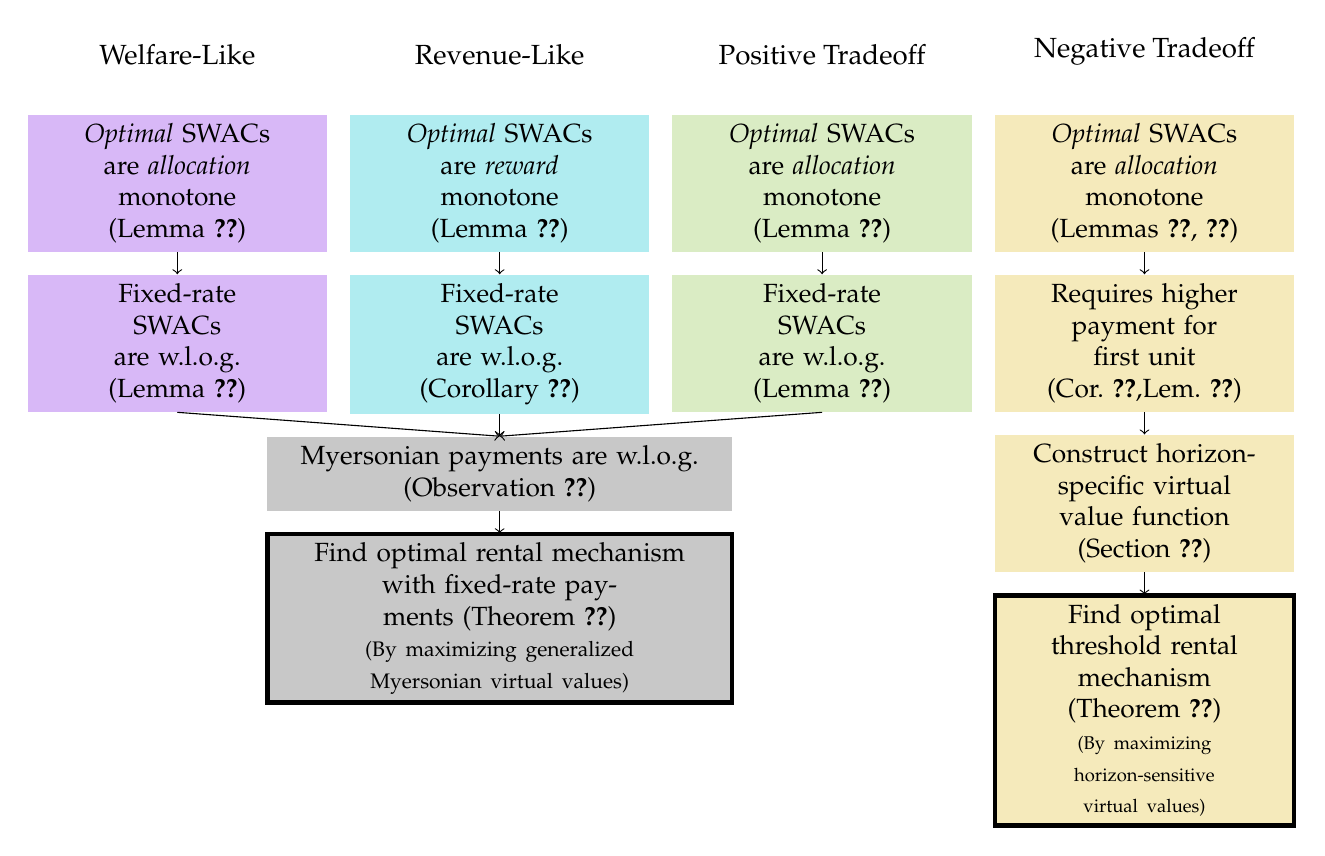
\begin{tikzpicture}[x=0.75pt,y=0.75pt,yscale=-1,xscale=1, % Reduced x and y scale
    node distance=8pt,
    purplebox/.style={fill={rgb, 255:red, 216; green, 184; blue, 247 }, fill opacity=1, minimum width=4cm, minimum height=0.8cm, text width=85pt, align=center,scale=0.95}, 
    greenbox/.style={fill={rgb, 255:red, 176; green, 236; blue, 240 }, fill opacity=1, minimum width=4cm, minimum height=0.8cm, text width=85pt, align=center,scale=0.95}, 
    bluebox/.style={fill={rgb, 255:red, 218; green, 236; blue, 196 }, fill opacity=1, minimum width=4cm, minimum height=0.8cm, text width=85pt, align=center,scale=0.95}, 
    yellowbox/.style={fill={rgb, 255:red, 245; green, 234; blue, 187 }, fill opacity=1, minimum width=4cm, minimum height=0.8cm, text width=85pt, align=center,scale=0.95}, 
    greybox/.style={fill={rgb, 255:red, 200; green,200; blue, 200 }, fill opacity=1, minimum width=2.5cm, minimum height=0.8cm, text width=170pt, align=center,scale=0.95}, 
    doubleborder/.style={draw, line width=0.2mm,  double=black, double distance=0.2mm} % Style for double border
    ]

% --- Nodes1 ---
\node (A1) [purplebox] {\textit{Optimal} \swacs\ are \textit{allocation} monotone\\(Lemma~\ref{lemma:welfare-like})}; 
\node (B1) [right=of A1, greenbox] {\textit{Optimal} \swacs\ are \textit{reward} monotone\\(Lemma~\ref{lemma:rev-like-rmono})};
\node (C1) [right=of B1, bluebox] {\textit{Optimal} \swacs\ are \textit{allocation} monotone\\(Lemma~\ref{lemma:pos-neg-tradeoff-samono})}; 
\node (D1) [right=of C1, yellowbox] {\textit{Optimal} \swacs\ are \textit{allocation} monotone\\(Lemmas~\ref{lemma:pos-neg-tradeoff-samono},~\ref{lemma:consumer-surplus-amono})};

% --- Text above nodes ---
\node [above=0.5cm of A1, align=center] {Welfare-Like};
\node [above=0.5cm of B1, align=center] {Revenue-Like};
\node [above=0.5cm of C1, align=center] {Positive Tradeoff};
\node [above=0.5cm of D1, align=center] {Negative Tradeoff};

% --- Nodes2 ---
\node (A2) [below=of A1, purplebox] {Fixed-rate\\\swacs\\are w.l.o.g.\\(Lemma~\ref{lemma:welfare-like})};
\node (B2) [below=of B1, greenbox] {Fixed-rate\\\swacs\\are w.l.o.g.\\(Corollary~\ref{corollary:rev-like-fr-wlog})}; 
\node (C2) [below=of C1, bluebox] {Fixed-rate\\\swacs\\are w.l.o.g.\\(Lemma~\ref{lemma:positive-tradeoff-fr-wlog})};
\node (D2) [below=of D1, yellowbox] {Requires higher payment for first unit\\(Cor.~\ref{cor:neg-tadeoff-fr-not-wlog},Lem.~\ref{lemma:neg-tradeoff-threshold-auction-truthful-and-optimal})}; 

% --- Nodes3 ---
\node (ABC1) [below=of B2, greybox] {Myersonian payments are w.l.o.g.\\(Observation~\ref{ob:fr-means-myerson})};
\node (D3) [below=of D2, yellowbox] {Construct horizon-specific virtual value function\\(Section~\ref{sec:threshold-mech})}; 

% --- Nodes4 ---
\node (ABC2) [below=of ABC1, greybox, doubleborder] {Find optimal rental mechanism\\with  fixed-rate payments (Theorem~\ref{thm:optima-fr-rental-mech})\\{\footnotesize (By maximizing generalized Myersonian virtual values)}};
\node (D4) [below=of D3, yellowbox, doubleborder] {Find optimal \\threshold rental mechanism (Theorem~\ref{theorem:threshold-mech})\\{\scriptsize (By maximizing }\\{\scriptsize horizon-sensitive}\\{\scriptsize  virtual values)}};

% --- Arrows 1---  
 \draw[->]       (A1.south) --(A2.north);
 \draw[->]       (B1.south) --(B2.north);
 \draw[->]       (C1.south) --(C2.north);
 \draw[->]       (D1.south) --(D2.north);

% --- Arrows 2---  
 \draw[->]       (A2.south) --(ABC1.north);
 \draw[->]       (B2.south) --(ABC1.north);
 \draw[->]       (C2.south) --(ABC1.north);
 \draw[->]       (D2.south) --(D3.north);

% --- Arrows 3---  
 \draw[->]       (ABC1.south) --(ABC2.north);
 \draw[->]       (D3.south) --(D4.north);

\end{tikzpicture}
\caption[Flow of proofs for welfare-like, revenue-like, positive tradeoff and negative tradeoff reward]{Flow of proofs for welfare-like, revenue-like, positive tradeoff and negative tradeoff reward. For each, we give monotonicity results (for either allocation or reward), 
establish the form of the optimal mechanism (w.l.o.g.),
and finally give an optimal rental mechanism.
Although some intermediate results appear to be the same across different types, each result is proven separately and leverages characteristics specific to the reward.}
\label{fig:flowchart}
\end{figure}

\tikzset{every picture/.style={line width=0.75pt}}
\usetikzlibrary{positioning}
% --- end proofs-flowchart.tex ---


The optimality of \fr payment schedules is no longer true for the class of negative tradeoff reward functions (e.g., consumer surplus $g(v,p) = v-p$). %where reward-monotonicity does not hold even for optimal \swacs 
For such reward functions, the designer is better off selecting only agents with high valuations for long rentals, but charging them low payments.
%Under \swir, the designer can select agents with valuations above a threshold $v_0$ by charging $v_0$ on the first unit (day), and zero on all subsequent days.
%Only agents with valuations $\geq v_0$ will be allocated, and the total payment will be $v_0$ regardless of the number of units sold, earning the designer a non-negative reward on the first unit and at least $v_0$ on all subsequent days.
%This high-valuation but low-payment screening effect cannot be achieved if we restrict the mechanism to fixed-rate payments.
We show that this screening effect cannot be achieved by mechanisms that charge fixed-rate payments,
and is necessary for optimality.
Nevertheless, we show that there is still an optimal mechanism with a simple structure:
%The resulting optimal rental mechanism remains simple, as it
we charge the entire cost of the rental on the first day, and zero on the remaining days.
%one high payment per agent and then zero.
%However 
Despite the simple structure, designing and analyzing mechanisms for negative tradeoff requires some new ideas---interestingly, we obtain it by optimizing a generalized horizon-dependent notion of Myersonian virtual values (see Section~\ref{sec:threshold-mech}).
One take-away message is that when the designer's objective is negative tradeoff, %so is aligned with that of the agent, 
utilizing \swir is no longer ``taking advantage'' of the agent but rather is beneficial for both designer and agent. 


As outlined above,
our first step is to reduce the rental mechanism design problem to a predetermined sequence of stagewise auctions with seller cost (\swacs),
and this is explained in Section~\ref{subsec:rental-to-swacs}.
Next, for each reward class, we establish some structural properties, and use them to derive an optimal \swac for that class.
The flow of the proof is illustrated in Figure~\ref{fig:flowchart}.







%:}
%In Section~\ref{subsec:rental-to-swacs}, we reduce the online rental mechanism design problem to an offline problem of designing a sequence of stagewise auctions \Inote{should it be SWAC here for consistency?}; in Section~\ref{sec:tech-overview-mono}, we analyze monotonicity in optimal \swacs\ and investigate whether \fr\ payment schedules are w.l.o.g.; in Section~\ref{sec:tech-overview-rental-mechs}, we derive the optimal rental mechanisms for all families of reward functions. In Section~\ref{sec:discussion} we summarize our techniques and discuss potential applications and directions for future research. Additional results and missing proofs appear in the appendices. 


\paragraph{Paper organization.}
We begin with a discussion of related work in Section~\ref{sec:related}.
In Section~\ref{sec:model}, we formally define the rental game, the rental mechanism, and stagewise auctions.
In Section~\ref{subsec:rental-to-swacs} we present our reduction from rental mechanisms to \swacs.
In Section~\ref{sec:properties}, we establish key properties of \swacs\ that are used throughout the paper and provide some intuition.
In Section~\ref{sec:tech-overview-mono}, we explore structural results on optimal \swacs\ for different classes of reward functions. In Section~\ref{sec:tech-overview-rental-mechs}, we derive optimal rental mechanisms using these results on \swacs.
In Section~\ref{sec:fr-gap}, we illustrate through examples how non-\fr\ pricing can significantly impact the designer's reward.
Finally, in Section~\ref{sec:our-techniques} we summarize our techniques, and in Section~\ref{sec:future} discuss potential applications and future research directions.
For brevity, some technical proofs are deferred to the appendix.
% --- end introduction.tex ---
% --- begin related-work.tex ---
\subsection{Related Work}
\label{sec:related}

\paragraph{Renting a Durable Good.} Renting is a fundamental mode of consumption, appearing in markets such as housing, books, and fashion. For a mechanism design perspective on the sharing economy, see \cite{OrenR21}. While selling mechanisms for durable goods have been extensively studied in economics \cite{doval2024optimal}, rental markets introduce a temporal component: assets remain available for future transactions, making opportunity cost a key factor \cite{beccuti2020optimality,cremer2003rental}. These differences place rental mechanisms within the broader realm of dynamic mechanism design, but unlike dynamic selling, rental mechanisms remain relatively unexplored. Our work contributes to filling this gap by formalizing a single-parameter rental game, highlighting connections to selling mechanisms while addressing novel design challenges.

\paragraph{Prophet Inequalities Over Time.}
Prophet inequalities have long been known to have deep connections to auction design~\cite{HajiaghayiKS07}, including applications to sequential posted-price mechanisms \cite{KleinbergW12}.
\cite{AbelsPS23} take a different approach: in ~\cite{AbelsPS23}, 
instead of selling goods to agents, they lend them over time.  In their model, each agent has an i.i.d.~valuation drawn from a known distribution, and the decision-maker selects an optimal lending strategy to maximize the expectation of the sum of valuations taken in each step (i.e., welfare). A crucial distinction is that their model does not involve payments, as valuations are revealed upon arrival. Their work provides a single-threshold algorithm that determines whether to lend to an agent and for how long.

In contrast, our model considers valuations drawn from different distributions across days, necessitating a more complex allocation structure (there can be multiple thresholds in the allocation rule). We design mechanisms that incorporate payments to ensure truthful behavior, which is essential when valuations are private. Furthermore, our work generalizes beyond welfare maximization by considering multiple economic objectives, including revenue and consumer surplus. Our results generalize their approach by addressing these challenges while maintaining incentive compatibility. 
 Recent works extend \cite{AbelsPS23} to a graph setting \cite{CristiO24} and improve approximation bounds \cite{perezsalazar2024}.
 
\paragraph{Stagewise Individual Rationality.} \Swir\ is a leading requirement in the literature on dynamic auctions (with repeated sales rather than a rental)~\cite{MirrokniLTZ16,MirrokniLTZ18,BravermanSW21}, and is sometimes referred to as \emph{per-round} individual rationality or \emph{ex-post IR}\footnote{Although ex-post IR usually does not relate to utility per stage, this is how it is defined in~\cite{MirrokniLTZ19}}.
 There are many economic reasons why agents might be \swir: for example, they might be unable to go into debt, or they might not have sufficient trust established with the designer to take on negative utility in the belief that the designer will keep to an agreement that will eventually result in positive utility.
~\cite{0001DMS18,AshlagiDH16,BalseiroML17}  study a slightly stronger notion of IR, in which the agent's utility in each stage, standalone, must be nonnegative\footnote{All of our results continue to hold if we require this stronger form of IR instead of \swir.} 
(see also \cite{PapadimitriouPP16,collina2024repeated}).
\cite{BravermanSW21} consider repeated auctions with adversarial valuations and per-round IR, assuming knowledge of total buyer valuations—a key distinction from our model.
\cite{0001DMS18} approximate revenue-optimal auctions under heterogeneous buyer behaviors, wheres we focus on rental mechanisms, where seller opportunity cost plays a central role, and explore optimal designs for multiple objectives beyond revenue, including welfare and consumer surplus.
 \cite{MirrokniLTZ16} develop bank account mechanisms for repeated combinatorial auctions with a form of IR that is not far from \swir. 
\cite{BalseiroML17} introduce martingale utility constraints, which we do not impose, allowing greater flexibility in the design of mechanisms.  \cite{krahmer2016optimality} study multi-unit contracts under ex-post participation constraints, though their model differs as buyers do not always know their valuations. 
Related sequential vs. simultaneous sales mechanisms appear in \cite{hausch1986multi,PapadimitriouPP16,AshlagiDH16}. 
\cite{BergemannCW17} focus on revenue-maximizing sequential auctions under ex-post IR constraints, which also allows for some sort of screening, but different from ours; their screening is used to offer different auction terms, depending on the type that the agent reports, and they have no allocation cost. They analyze when static contracts are optimal and when dynamic ones (i.e. with screening) are optimal, depending on the valuation distribution. 


\paragraph{Dynamic auctions.} Dynamic auctions are essentially repeated auctions that are optimized over time, adapting payments based on past events \cite{bergemann2019dynamic,bergemann2010dynamic}. \cite{MirrokniLTZ19} study dynamic auctions with multiple buyers and sequentially arriving items.
 \cite{0001DMS18}  examine revenue-maximizing repeated auctions with a single buyer, assuming limited trust in the seller. In contrast, we assume full commitment, enabling exact optimal mechanisms.
\cite{DevanurPS15} consider a repeated auction to a single seller with a fixed value for the item, drawn from a known distribution, which is similar to our dynamic auction, but does not include a seller cost function. Another major difference is that they consider only cases where the seller does not have full commitment over future prices, which greatly limits the designers' capabilities. Additionally, they consider a Perfect Bayesian Equilibria (which is why they don't consider full commitment), whereas we consider dominant strategy equilibrium.  \cite{MirrokniLTZ18} focus on non-clairvoyant mechanisms, restricting future distributional knowledge, whereas our model assumes full knowledge, which is key for mechanism design.

\paragraph{General seller costs.} A general cost environment is one in which the designer must pay a service cost $c(x)$ for an allocation $x$, and is defined by~\cite[Chapter 3]{hartline2013mechanism}, and considered for example by~\cite{krahmer2016optimality}, who consider some form of a repeated auction, but in which the buyer's valuation has only 2 possible values.

\paragraph{Additional related work.}
\cite{FeldmanGL15} studies combinatorial online auctions where buyers with valuations drawn from known priors arrive sequentially and purchase their utility-maximizing bundle at initially defined posted prices. Their work focuses on achieving an approximation algorithm for social welfare maximization. While~\cite{FeldmanGL15} explores simple posted price mechanisms for combinatorial goods, our work focuses on dynamic mechanisms for the rental of a single asset under stagewise individual rationality, considering a broader range of reward functions

% --- end related-work.tex ---
% --- begin rental-and-swac.tex ---
\section{Our Model}\label{sec:model}

In this section we formally define the rental game model,
as well as stagewise auctions with seller cost (\swacs), which model the designer's interaction with a single agent. 
Throughout,
we let $\sqrrange{n} =\set{0,\ldots,n}$ and $\psqrrange{n} = \set{1,\ldots,n}$. 

\subsection{The Rental Game}\label{subsec:rental}

Fix a domain $\V$ of possible nonnegative agent valuations.
An \emph{$(n, \boldsymbol{\D}, \g)$-rental game}
is defined by a length $n \geq 0$, which is the timeframe over which the game is played;
a sequence of distributions
of agent valuations,
$\boldsymbol{\D} = \D_1,\ldots,\D_n$ supported over $\V\subseteq\preals$, one for each day; 
and a \emph{reward function} $\g$,
whose cumulative value over time the designer aims to maximize.



The game consists of \emph{days},
on each of which a new agent $i$ arrives with an independent valuation $v \sim \D_i$, interacts with the designer, and is either allocated the asset for some number of days under some payment schedule, or turned away.
The \emph{payment schedule}
is a sequence of payments
$p = (p_1,\ldots,p_x)$,
where $x$ is the length of the allocation.
We refer to the number of remaining days at some point in the game as the \emph{horizon}.

Each distribution $\D_i$ is assumed to have a probability density function (pdf) and to be supported on a single continuous interval (not necessarily the same interval for all distributions).
We also make the following assumptions on the reward function $g$:
\begin{enumerate*}
    \item It is normalized so that $g(0,0) = 0$;
    \item It is non-decreasing in its first argument, the valuation;
    \item For all valuations $v \in \V$,
    the function $g(v, \cdot) : \preals \rightarrow \preals$ is linear (in the payment).
\end{enumerate*}
The last constraint captures the fact that the designer is motivated only by the \emph{total} payment,
not the payment \emph{schedule},
so that for any two payment schedules $(p_1,\ldots,p_x)$ and $(p_1', \ldots, p_{x}')$ for the same allocation $x$,
if $\sum_{i = 1}^x p_i = \sum_{i = 1}^{x} p_i'$,
then $\sum_{i = 1}^x g(v, p_i) = \sum_{i = 1}^{x} g(v, p_i')$ for any valuation $v$.
%(we elaborate on our requirements of $g$ in Section~\ref{subsec:design_objective_constraints}).


Next we define \emph{stagewise auctions},
the mechanism by which the designer negotiates with one individual agent;
then, in 
Section~\ref{sec:rental_mech_definitions}, we 
use stagewise auctions to define \emph{rental mechanisms},
the overall mechanism by which the designer interacts with all $n$ agents over the $n$ days of the game.


%\section{The Rental Game and the Stagewise Auction with Cost}


%\subsection{Review: Stagewise Auctions with Seller Cost}
\subsection{Stagewise Auctions with Seller Cost}
\label{subsection:auction}

\paragraph{Stagewise auction settings.}
A \emph{$(n,\D,\g,c)$-stagewise auction setting with seller cost} (\emph{\swac setting} for short)
features a single \emph{seller} (a.k.a. designer) and a single \emph{buyer} (a.k.a. agent).
The seller wishes to sell up to $n$ units of a single item,
\emph{over time},
one unit per day.
The buyer has some valuation $v$ per unit, drawn from a distribution $\D$
supported on $\V\subseteq \mathbb{R}_{\ge 0}$.
If $\V$ is unbounded from above, we abuse notation by writing $\sup\V=\infty$.
The \swac\ setting is publicly known, but the valuation $v$ is known only to the buyer.

The seller has a \emph{reward function} $g(\cdot,\cdot)$
mapping a valuation~$v$ and a payment $p$ to the seller's reward from selling
a single unit (on a single day) at price $p$ to an agent with valuation $v$. The reward is additive,
so that the seller's reward from selling $k$ units at prices $p_1,\ldots,p_k$ to an agent with valuation $v$ is given by $\sum_{i = 1}^k g(v, p_i)$.
However, 
the seller also
incurs a \emph{cost} $c:\sqbr{n}\rightarrow\preals$,
mapping the number of units sold to the overall production cost that the seller pays. 
The cost function is normalized so that $c(0)=0$, and it is non-decreasing in the number of units sold.
We distinguish between the \emph{gross reward} $\sum_{i = 1}^k g(v,p_i)$ of the designer from selling $k$ units, and their \emph{net reward}, which is the gross reward minus the cost of producing the $k$ units (see below).
For brevity, in the sequel,
we use the term \emph{reward} to refer to the designer's net reward.








%%%%%%%%%%%%%%%% PREV VERSION %%%%%%%%%%%%%%%%%%%%
\hide{
Informally, our auction setting has a single buyer (a.k.a.~\emph{agent}), single seller (a.k.a.~\emph{designer}), and 
$n$ units of a single item of which multiple can be sold, one unit per time period (``day'').
The buyer submits a bid from some bidding set defined by the designer. 
Based on the buyer's bid, the auction determines a sequence of up to $n$ prices $(p_1,p_2,\dots)$;
on each day $i$, the seller sells a unit of the item to the buyer for price $p_i$. 
The seller incurs a \emph{cost} for the total number of units produced and sold to the buyer. 
The most important feature of the setting is that, as in~\cite{BravermanSW21,MirrokniLTZ19,MirrokniLTZ16}, we assume that the agent must maintain individual rationality at all times (in Appendix~\ref{appendix:oir} we analyze the case in which the agent only needs to maintain \emph{overall} individual rationality). 
The formal definitions are as follows.

\paragraph{Stagewise auctions with seller cost.} 
Let $\V\subseteq \mathbb{R}_{\ge 0}$ be a domain of possible agent valuations. If $\V$ is unbounded, we abuse notation by writing $\sup\V=\infty$. An \emph{$(n,\D,\g,c)$-stagewise auction setting with seller cost} (stagewise auction or \swac\ for short) has a single seller (designer) who can sell up to $n$ units of an item, one per day, %\Bnote{same comment about production at once or per day}, 
and a single buyer (agent) with valuation $v\in \V$ per unit. We sometimes refer to such a buyer as \emph{agent~$v$}. Valuation $v$ is drawn from distribution $\D$ supported over~$\V$.
The seller has a \emph{reward} function $\g$ mapping a valuation~$v$ and a payment $p$ to the seller's reward from selling
a single unit (on a single day) at price $p$ to an agent with valuation $v$. The reward is additive,
so that the seller's reward from selling $k$ units at prices $p_1,\ldots,p_k$ to an agent with valuation $v$ is given by $\sum_{i = 1}^k g(v, p_i)$  (we elaborate on our requirements of $g$ in Section~\ref{subsec:design_objective_constraints}).
%the $i$th unit at price $p_i$. %, for example revenue (we discuss our requirements from $g$ below).  
The seller also has a \emph{cost} function $c:\sqbr{n}\rightarrow\preals$, mapping the number of units sold to the overall production cost that the seller incurs. 
The cost function is normalized so that $c(0)=0$, and it is non-decreasing.
The \swac\ setting is publicly-known, while the valuation $v$ is known only to the buyer. 

%The auction deducted from the reward. %designer's total value. 

%Where clear from the context, we refer to an $(n,\D,\g,c)$-dynamic auction setting with general cost simply as a dynamic auction (or $n$-auction) setting. In terms of who knows what, the auction setting is publicly-known, while the valuation $v$ is privately-known to the buyer. 
}

%%%%%%%%%%%%%%%%%%%%%%%%%%%%%%%%%%%%%%%%%%%%%%%%%%%%%%%%%

\paragraph{Stagewise auctions.}
In its most general form, the negotiation between the seller and the buyer in a stagewise auction may feature both randomness and daily interaction: each day,
the seller negotiates with the buyer and decides whether to sell the buyer
one unit that day, and at what cost.
The next day they negotiate for the next unit, and so on,
until eventually either all $n$ units are sold or the seller decides not to sell the buyer any more units and the buyer leaves.
To simplify the exposition, we focus on a simplified and deterministic
version where the buyer submits a single bid on the first day,
and the seller then decides how many units
to sell in total (still one unit per day), and what payment to charge on each day.
We prove in Appendix~\ref{app:generelizations-and-definitions} that this simplified form is without loss of generality.

Formally, given a \swac\ setting $(n,\D,\g,c)$,
a \emph{stagewise auction with seller cost (\swac)} $\A:\B\rightarrow \left(\preals\right)^\ast$
for this setting
is a (deterministic) mapping that takes a bid $b\in \B$, where $\B$ is a bidding set defined by the seller, and outputs a
\emph{payment schedule} $\A(b) = (p_1, \ldots,p_x)$,
where $x \leq n$ is the the number of units sold to the buyer.
Each $p_i \in \preals$ is the payment charged for the $i$-th unit on day $i$.
The buyer 
is assumed (w.l.o.g.) to be deterministic,
and
%ties in the buyer's utility are broken in favor of the seller, and further ties are assumed to be broken in a manner that is consistent amongst buyers. 
ties in the buyer's utility are broken in favor of the seller.
Our goal is to design a \swac\ that maximizes in expectation the seller's \emph{net reward}, which is the total reward over all units sold, minus the cost of the allocation.
%The notations for the dynamic auction are the same as in the subrental: 



\paragraph{Notation and terminology.}

Given a stagewise auction $\A$ and an buyer $v$ that makes bid $b$, we use the following notation and terminology (omitting $\A$ where clear from the context):
\begin{itemize}
    \item The \emph{allocation}, $\x[\A]{b}$, is the number of units allocated to the buyer.
    \item The \emph{total payment} of the buyer is denoted $\p[\A]{b} = \sum_{i = 1}^{\x[\A]{b}} p_i$, where $(p_1,\ldots,p_{\x[\A]{b}})$ 
    are the payments charged by the seller.
    \item The \emph{cumulative utility} of the buyer
    from the first $i \leq \x{b}$ 
    units they are allocated is denoted
    $\utili[\A]{i}{v}{b} = i \cdot v - \insumof{j}{1}{i} p_j$.
    \item The \emph{overall utility} of the buyer is $\util{v}{b}=\utili{\x{b}}{v}{b}$.
\item The seller's net reward is denoted by
$\rew[\A]{v}{b} = \insumi{1}{\x{b}}\g(v,p_i)-c(\x{b})$.
\end{itemize}

To simplify the notation, we let $\trew[\A]{v}$ denote the seller's net reward when an buyer with valuation $v$ bids optimally (i.e., in a manner that maximizes the buyer's utility).
%\coloneq\rew{v}{\bid{v}}$ denote the seller's net reward when buyer $v$ bids optimally.
The seller aims to maximize $\E[\A]=\E_{v\sim\D}[\trew[\A]{v}]$. We say that a \swac is \emph{truthful} if bidding truthfully is a weakly-dominant strategy for an agent with any valuation.
Finally, for ease of exposition, we may refer to an $(n,\D,\g,c)$-stagewise auction as an $n$-auction, when the context is clear.




\paragraph{Stagewise individual rationality (\swir).}
The key feature of our model is that agents are not willing to temporarily incur negative utility at any point in time.
Formally, a \swir agent with valuation $v$
will not make bid $b \in \B$
if there exists a day $1 \leq i \leq \x[\A]{b}$
on which $\utili[\A]{i}{v}{b} < 0$.

\paragraph{Filters.}
The filter 
represents the highest cumulative average payment encountered at any day and is given by $\f{b}=\max_{\ell\leq\x{b}}
        \insumi{1}{\ell}p_i/\ell$.
A \swir\ agent will not submit a bid resulting in a negative cumulative utility at any day, hence they can only submit a bid $b$ if $\f{b}\leq v$. 
For example, if the payments induced by some bid are $(3,4,2)$, 
the cumulative average payments at each timestep are: $
\frac{3}{1}, \frac{3+4}{2} = 3.5$ and $ \frac{3+4+2}{3} = 3$.
Thus, the \emph{filter for this bid} is \( \max \{ 3, 3.5, 3 \} = 3.5 \), which occurs after the first two days. 
Consequently, an agent with valuation \( v < 3.5 \) cannot submit this bid.
In essence, the filter served as a ``barrier to entry'' for making bid $b$:
it is the smallest valuation of any \swir\ agent that can afford
to place bid $b$,
without going into negative utility at any point. As a design tool, 
where truthfulness is concerned,
they are useful in preventing
{overbidding},
not {underbidding}. Observe that a payment schedule can, w.l.o.g., consist of a high payment on the first day—thereby defining the filter—with the remaining payments spread evenly over the subsequent days.

\paragraph{Finite-menu stagewise auctions.}
Our monotonicity results for positive and negative tradeoff are restricted to
\swacs that have a finite number of options:
there is a finite number of payment schedules
that the seller offers.
W.l.o.g., such \swacs can be represented as follows:
we say that a \swac\ is \emph{finite-menu}
%a \emph{\finauc}
if it is truthful
and its allocation function has the form
$\I_1 \mapsto x_1,\ldots, \I_k \mapsto x_k$,
where
$\I_1 = [ t_1, t_2 ), \ldots, \I_k = [t_k, t_{k+1}]$ are adjacent non-overlapping intervals,
with $\inf \V = t_1 < t_2 < \ldots < t_k < t_{k+1} = \sup \V$,
and $x_i$ is the allocation for any bid in the interval $\I_i$.
The payment schedule associated with all bids in an interval $\I_i$
is the same;
we denote by $p_i$ the total payment for a bid in $\I_i$.
Although technically agents submit bids in $\V$ (the auction is truthful),
since all bids in a given interval lead to the same outcome,
it is convenient to think of a bid as the interval $\I_i$ to which it belongs,
and accordingly we sometimes use the notation $\util{v}{\I_i}$.

We say that a \finauc\ is \emph{finite-menu optimal} (or \emph{FM-optimal}, for short)
if it is optimal within the family of all \finaucs.


\subsection{Rental Mechanisms}\label{sec:rental_mech_definitions}
 A \emph{rental mechanism} for the $(n, \boldsymbol{\D},\g)$-rental game is 
 a mapping $\mech{M}$ that
 takes the current history $\history$ of the game,
 and if the asset is currently available,
 returns a \swac\ $\M(\history)$
 that is used to negotiate with the current day's agent.
 The number of units in the \swac\ is equal to the
 number of days remaining in the game,
 but the other parameters (the distribution, reward function and cost function) can be chosen arbitrarily by the designer.
   The allocation returned by the \swac\ determines the number of days the current agent rents the asset, and its payments specify the sequence of daily rental fees charged to the agent.
  
%As shown in Appendix~\ref{app:rental-to-swacs}, without loss of generality the \swacs\ of a rental mechanism can be predetermined. Hence, a rental mechanism can be viewed as a sequence of deterministic \swacs: ${\A_n,\dots,\A_1}$, where $\A_i$ is applied at horizon $i$ when the asset is available.

Let $v_1,\ldots,v_n$ be the valuations of the $n$ agents that arrive over the $n$ days,
and suppose that under the mechanism $\M$
the designer rents the item to agent $j_i$ on day $i$ and charges payment $p_i$.
If the asset is not rented out to any agent on day $i$, then $j_i = \bot$ and $p_i = 0$.
The designer's \emph{reward}
is given by 
$\trew[\mech{M}]{v_1,\dots,v_n} = \sum_{1 \leq i \leq n : j_i \neq \bot} g( v_{j_i}, p_i)$.
The designer’s objective is to maximize their expected reward,
$
\E\sqbr{\trew[\mech{M}]{v_1,\dots,v_n}},
$ 
sometimes denoted $\E[\M]$ for short.

Throughout the remainder of the paper, we purposefully use some of the \swac notation of Section~\ref{subsection:auction} in the context of rental mechanisms as well, since a rental mechanism consists of a sequence of \swacs.



% Once we showed that \swacs are deterministic w.l.o.g., we observe that also agents are. This 
% \begin{observation}
%     In a deterministic \swac, any agent, with any valuation, has a weakly dominant strategy that is deterministic.
% \end{observation}

% \begin{lemma}\label{lemma:in_deterministic_auction_agent_is_det}
%     In a deterministic \swac, every agent has a weakly dominant strategy that is deterministic.
% \end{lemma}
% \begin{proof}
%     Let $\A$ be a deterministic $(n,\D,\g,c)$-auction, and let $v$ be the valuation of an agent. We prove by induction on the number of units remaining, that it is a weakly dominant strategy for the agent to be deterministic. For the base of 0 units remaining this is trivial, so suppose this is correct when there are up to $n-k$ units remaining, and prove for $n-k+1$.
    
%     Fix history $\history_{k}$ of the first $k-1$ bids, and suppose that there are $n-k+1$ units remaining and the auction is not done yet. The auction is deterministic, thus the seller offers a deterministic bidding set $\B_k$ and mapping $\spay_k:\B\rightarrow\preals$. Denote by $U_{[i,j]}$ the agent's utility received from units $i,\dots,j$ (if $i>j$ or these units were not sold to the agent, then this is defined as 0). Denoting by $\history_kb$ the concatenation of the first $k-1$ bids together with the $k$th bid $b$ for any bid $b\in\B_k$, it holds that, if $b\neq\psi$:
%     \begin{align*}
%         \E\sqbr{U_{[1,n]}\mid\history_kb}&=\E\sqbr{U_{[1,k-1]}\given\history_kb}+\E\sqbr{U_{[k,k]}\given\history_kb}+\E\sqbr{U_{[k+1,\dots,n]}\given\history_kb}\\
%         &=\E\sqbr{U_{[1,k-1]}\given\history_k}+\brackets{v-\spay_k(b)}+\E\sqbr{U_{[k+1,\dots,n]}\given\history_kb}
%     \end{align*}
%     If $b=\psi$ we have simply $\E\sqbr{U_{[1,n]}\mid\history_kb}=\E\sqbr{U_{[1,k-1]}\given\history_k}$.

%     The first term $\E\sqbr{U_{[1,k-1]}\given\history_k}$ is constant since the history is fixed. The final term $\E\sqbr{U_{[k+1,\dots,n]}\given\history_kb}$ relates to the agent's utility from the final $n-k$ units, in which the agent can bid deterministically, due to the induction hypothesis, leading to a deterministic function mapping $b$ to some fixed utility.
%     It follows immediately that the agent can select, using a deterministic tie-breaking rule, a bid from
%     \begin{align*}
%         \argmax{b\in\B_k}\E\sqbr{U_{[1,n]}\mid\history_{k}b}
%     \end{align*}
%     in order to maximize his expected utility, completing the proof.
    
%     % Fix history $\history_{k}$ of selling the first $n-k$ units, and suppose that there are $k$ units remaining and the auction is not done yet. The auction is deterministic, thus the seller offers a deterministic allocation function $\alloc:\B\rightarrow\sqrrange{k}$ and a deterministic payment function $\pay:\B\rightarrow\preals$ for the next bundle, where $\B$ is the bid space. In general, denote by $U_{[i,j]}(b)$ the agent's utility received from units $i,\dots,j$ (if $i>j$ or these units were not sold to the agent, then this is defined as 0). It holds that, for current bid $b$:
%     % \begin{align*}
%     %     \E\sqbr{U_{[1,n]}(b)\mid\history_{k}}=\E\sqbr{U_{1,n-k}\given\history_{k}}+\E\sqbr{U_{[n-k+1,\dots,n-k+\x{b}]}\given\history_{k}}+\E\sqbr{U_{[n-k+\x{b}+1,\dots,n]}\given\history_{k}}
%     % \end{align*}

%     % The first term $\E\sqbr{U_{1,n-k}\given\history_{k}}$ is a constant since the history is fixed. The final term $\E\sqbr{U_{[n-k+\x{b}+1,\dots,n]}\given\history_{k}}$ relates to the agent's utility from the final $k-\x{b}$ units. If $\x{b}=0$ the auction ends earlier and this term is zero, and if $\x{b}>0$, then the last term relates to the utility from a point in which there are \emph{less} than $k$ units remaining. Thus from the induction hypothesis, the term $\E\sqbr{U_{[n-k+\x{b}+1,\dots,n]}\given\history_{k}}$ depends only on $b$. Finally, the middle term $\E\sqbr{U_{[n-k+1,\dots,n-k+\x{b}]}\given\history_{k}}=\x{b}v-\p{b}$ which depends only on $b$, since $\alloc$ and $\pay$ are deterministic.

%     % It follows immediately that the agent can select, using a deterministic tie-breaking rule, a bid from
%     % \begin{align*}
%     %     \argmax{b}\E\sqbr{U_{[1,n]}(b)\mid\history_{k}}
%     % \end{align*}
%     % in order to maximize his expected utility.
% \end{proof}

% Finally we show that back-and-forth interaction is unnecessary, and truthfulness is w.l.o.g.

% \begin{lemma}\label{lemma:truthful_auction_wlog}
%     A deterministic $(n,\D,g,c)$-auction can be converted into a truthful auction, with only a single bid at the start of the auction that conserves the allocation and payment of each agent, and yields the same designer reward as the original auction, for every agent.
% \end{lemma}
% \begin{proof}
%      Let $\A$ be a deterministic $(n,\D,\g,c)$-auction. Since $\A$ is deterministic, there is a deterministic mapping from each valuation to an allocation and payment schedule.
     
%      Define a new auction $\A'$ which accepts a valuation $v$ at the beginning of the auction. In the following stages, it sells exactly the same number of units with the same payment schedule as an agent with valuation $v$ would have ended up with in $\A$. Specifically, for each $v\in\V$, it holds that $\x[\A']{v}=\xhat[\A]{v}$,  $\p[\A']{v}=\phat[\A]{v}$ and $\f[\A']{v}=\fhat[\A]{v}$. We will show that $\A'$ is indeed truthful: Suppose there's a bid $w\in\V$ such that $\util[\A']{v}{w}>\util[\A']{v}{v}$. By definition of $\A'$, and in either IR setting, this would mean that $\util[\A]{v}{\strat[\A]{w}}>\util[\A]{v}{\strat[\A]{v}}$, which is a contradiction to the utility maximization of $v$ in $\A$. Thus it is a weakly dominant strategy for agents to bid truthfully.

%      Since $\A'$ is truthful and the allocations and payments are equal for every agent between both auctions, it holds that $\E[\trew[\A']{v}]=\E[\trew[\A]{v}]$, completing the proof.
% \end{proof}
% --- end rental-and-swac.tex ---
% --- begin technical-overview-monotonicity.tex ---
% \section{Technical Overview}\label{sec:tech-overview}

%We give a high-level overview of our results characterizing the structure of optimal rental mechanisms and stagewise auctions, and then explain how we use them to find optimal mechanisms for the various reward classes.



\hide{
\paragraph{Reducing the rental game to a sequence of auctions.}
Our first step is to reduce the rental mechanism design problem to a predetermined sequence of stagewise auctions with seller cost (\swacs),
\Rnote{Is this the first occurrence of \swacs now? If so, need more setup.}\Bnote{what do you mean now? Section 2 describes the model, including \swacs}
one for each day $i = 1,\ldots,n$; 
the \swac\ for the $i$-th day will be used if the asset is free on that day to negotiate with the agent that arrives (otherwise, the agent is turned away).
The $i$-th \swac\ has a \emph{time horizon} of $n - i+1$ days, 
and a \emph{seller cost} that reflects,
for each possible allocation $x \in \set{0,\ldots,n-i+1}$
of rental days to the current agent,
the expected loss of reward from turning away future agents that arrive on days $i+1,\ldots,i+(x-1)$.

Having reduced the rental game to a sequence of \swacs,
we can now solve each one in isolation. Under \oir, 
\Rnote{Maybe set up more, depending on how prominent \oir ends up being in the intro}
it is not hard to show that
Myerson's unique payment rule~\cite{myerson1981optimal} applies, allowing a fairly straightforward solution:
the \emph{(ironed) virtual value for revenue} defined by Myerson allows us to find an allocation rule that maximizes the revenue for each valuation $v$ \emph{pointwise}, since the (average, per unit) expected payment is equal to the expected virtual value of the agent.
In contrast, as we saw in Example~\ref{ex:intro-example}, under \swir\ the unique payment rule is not required \Rnote{What does that mean exactly? Is ``not required'' = ``not necessarily the only payment rule that a truthful auction can use''?},
and therefore the equality between expected payment and expected virtual value that holds for standard truthful auctions is no longer true.
We would like to determine in which cases Myerson's payment rule
is optimal: we know that it is not necessarily used in any truthful \swac, but we ask whether it is used w.l.o.g.\ by the \emph{optimal} \swac.
When this holds, it  allows us to build upon Myerson's technique, define virtual values for each reward class, and use them to find an optimal rental mechanism.
It turns out that an important question along the way is whether for a given reward class, \fr \swacs\ are optimal \Rnote{\fr \swacs\ defined?}:
in each of the three cases where they are (revenue-like, reward-like and positive tradeoff),
we are able to show that Myerson's payment rule is optimal (the proof is different for each of the three reward classes).

For each of the four classes,
we first prove a \emph{monotonicity} result for the class,
either with respect to the allocation (for welfare-like, positive and negative tradeoff), or with respect to the designer's reward (for revenue-like reward).
In the case of welfare-like, revenue-like and positive tradeoff reward, we then leverage monotonicity to prove that an optimal \swac\ for any reward function from the class is fixed-rate w.l.o.g. The proof is different for each class,
but once we establish that fixed-rate \swacs\ are optimal,
the process of finding the optimal mechanism is the same for these three classes, and indeed maximizes generalized Myersonian virtual values.


For negative tradeoff, we show that fixed-rate \swacs\ are \emph{not} optimal,
and in fact the gap between the optimal reward and the reward that a fixed-rate \swac\ can achieve is large. However, using allocation-monotonicity,
we show that the payment schedule of an optimal \swac\ is still not too complex: it takes the form of a \emph{threshold mechanism},
where all payment is charged up-front on the first day, and furthermore, the payment charged under any bid is equal to the minimum valuation of an agent that would make this bid.
We are then able to use this structure to find an optimal mechanism for negative-tradeoff \swacs.
Figure~\ref{fig:flowchart} shows the flow of the results in our paper.
}


% For each of the four classes,
% we first prove a \emph{monotonicity} result for the class,
% either with respect to the allocation (for welfare-like, positive and negative tradeoff), or with respect to the designer's reward (for revenue-like reward).
% In the case of welfare-like, revenue-like and positive tradeoff reward, we then leverage monotonicity to prove that an optimal \swac\ for any reward function from the class is fixed-rate w.l.o.g. The proof is different for each class,
% but once we establish that fixed-rate \swacs\ are optimal,
% the process of finding the optimal mechanism is the same for these three classes.


% Want to use Myerson's payment rule,
% even though Lemma doesn't apply:
% Myerson gives a way to reduce the problem of choosing both allocation and payment per bid
% to the problem of choosing an allocation alone:
% Myerson defines a \emph{virtual value}, which captures the expected revenue \emph{per unit} that the designer can obtain from Myerson's payment rule.
% (Using uniqueness)
% This allows us to focus on the allocation (the number of units).
% Then, relying on \emph{allocation-monotonicity},
% we can maximize the revenue in a pointwise manner:
% for each valuation $v$,
% we find the allocation that maximizes the revenue from agents with that valuation,
% ignoring all other valuations.
% %, and shows that the expected revenue is equal to the expected virtual value.

% $E[\varphi(v)x(v)]=\E[p(v)]$

% maximize the designer's reward in a pointwise manner, by defining a \emph{virtual value} that expresses the designer's reward from a given allocation

% is optimal. (Not even necessarily its uniqueness)



\section{From Rental Games to Stagewise Auctions with Cost}\label{subsec:rental-to-swacs}

In this section we  explain how we reduce the rental mechanism design problem from an \emph{online} problem to an \emph{offline} one by showing that the designer can fix in advance a sequence: $\A_1,\ldots,\A_n$ of optimal stagewise auctions (\swacs),
where $\A_i$ is to be used to negotiate with the agent that arrives on day $i$ if the asset is available that day. We remark that this reduction holds for \emph{any} reward function, even if it does not satisfy the assumptions in Section~\ref{subsec:rental}. 
The full results for this section appear in Appendix~\ref{app:rental-to-swacs}.



The first step in our reduction is to show that w.l.o.g.,
an optimal rental mechanism is a \emph{fixed} (i.e., predetermined) sequence of \swacs:
because agent valuations are independent of one another,
an optimal rental mechanism can be \emph{history-independent},
meaning that 
although we do not know in advance whether the asset will be available to rent on a given day and what we did with the asset prior to that day,
we can decide in advance what the mechanism should do \emph{if} the asset is available that day,
regardless of the history up to that day.
Next we show that w.l.o.g., the \swac\
for the $i$-th day uses a specific seller cost function,
which captures
the designer's \emph{opportunity cost} ---
the expected loss of future reward incurred by renting the asset to the current agent.
If the designer rents out the asset for $x\geq1$ days at horizon $n$,
they forgo the expected reward from days $n-1,\dots,n-(x-1)$, since the asset is unavailable during this period. 
However,
the asset becomes available again at horizon $n - x$, 
so the designer can gain the expected reward from that point onward.
The \emph{opportunity cost} is defined as the difference between these two expected rewards:

\begin{definition}
An $(n,\boldsymbol{\D},\g)\textnormal{-over-time cost function}$ is defined as:
\begin{align*}
    c^{\boldsymbol{\D}}_{n,\g}(x)
    &=
    \begin{cases}
        R^{\boldsymbol{\D}_{\text{last }n-1},\g}_{n-1}-R^{\boldsymbol{\D}_{\text{last }n-x},\g}_{n-x},&\text{if }x\geq 1\\
        0,&\text{otherwise}
    \end{cases} %\right}
    \qquad
    =
    \qquad
    R^{\boldsymbol{\D_{\text{last }n-1}},\g}_{n-1}-R^{\boldsymbol{\D}_{\text{last }n-\max\{x,1\}},\g}_{n-\max\{x,1\}},
\end{align*}
where $R^{\boldsymbol{\D},\g}_m$ denotes the expected reward of an optimal $(m,\boldsymbol{\D},\g)$-rental.
\label{def:cost-function}
\end{definition}
For clarity, we may omit superscripts and subscripts when the context is unambiguous.

The reduction from rental games to \swacs\ is summarized by the following theorem:

\begin{theorem}\label{theorem:rental_as_auctions}

    For all $h\in\psqrrange{n}$, let $\A_h$ be an optimal $\brackets{h,\D_h,\g,c_{h,\g}^{\boldsymbol{\D}}}$-stagewise auction with over-time cost. Then, the rental mechanism $\brackets{\A_n,\dots,\A_1}$ is optimal for the $(n,\boldsymbol{\D},\g)$-rental game.

\end{theorem}


The remainder of this technical overview describes how to find an optimal \swac\ under welfare-like, revenue-like, positive tradeoff or negative tradeoff reward.
However, our results are not restricted to the over-time cost from Definition~\ref{def:cost-function}:
they apply under any seller cost function, as long as the reward function
of the \swac\ is from one of the four classes.

\section{Useful Properties of Stagewise Auctions}\label{sec:properties}

The following propositions are used throughout,
and help establish some intuition for the structure of \swacs
and the way agents behave in them. These properties help establish key characteristics of truthful \swacs and illustrate how payments, allocations, and filtering interact.

\begin{proposition}
    \label{prop:decreasing-payments}
    In any truthful \swac,
    if two bids $w < v$
    receive the same allocation, $\x{w} = \x{v}$,
    then 
    the higher-valuation agent pays less,
    that is,
    $\p{w} \geq \p{v}$.
\end{proposition}
\begin{proof}
    Suppose $\p{w} \neq \p{v}$ (otherwise we are done).
    Agent $v$ can withstand any payment schedule that agent $w$ can (as $v > w$),
    but since the \swac is truthful,
    we know that $v$ chooses not to bid $w$.
    The allocations for the two bids are the same, so the only reason agent $v$ prefers to bid $v$ rather than $w$ is that
    they pay less,
    that is,
    $\p{w} > \p{v}$.
\end{proof}

\begin{proposition}
    \label{prop:benefit_swap}
%    Let $w' < w < v$ be valuations,
%    and let $\A$ be a (non-truthful) \swac
%    where
%    $\x{w'} < \x{w}$, but
%    agent $v$ bids $w'$ and not $w$ (despite receiving a lower allocation).
%    Then agent $w$ is not truthful in $\A$.
Consider a (not necessarily truthful) stagewise auction $\A$,
let $w < v$ be valuations,
    and let $b, b'$ be two bids such that $\x{b} > \x{b'}$.
    Then the benefit that agent $w$
    derives by switching 
    from bid $b$ to bid $b'$
    % from bid $b'$ to bid $b$
    exceeds that of agent $v$,
    that is,
        $\util{w}{b'} - \util{w}{b}
        >
        \util{v}{b'} - \util{v}{b}
        $.
    \end{proposition}
\begin{proof}
    For any valuation $z$,
    \begin{equation*}
        \util{z}{b'} - \util{z}{b}
        =
        \left( \x{b'} - \x{b} \right) \cdot z - \left( \p{b'} - \p{b} \right).
    \end{equation*}
This is strictly 
% increasing
decreasing
in $z$, and the claim follows.
\end{proof}

Observe that the marginal utility of allocating an additional unit at some fixed price is higher for a ``stronger'' agent than for a ``weaker'' one. This implies that, in general, the stronger agent is more willing to accept a larger allocation than the weaker agent. Thus, if a weaker agent $w$ receives more units than a stronger agent $v$ in a truthful auction, it is because the weaker agent was filtered out from bidding similarly to the stronger agent. Formally, $\p{v} \geq \f{v} > w$ and $\x{v}>1$, as the filter would not be possible otherwise. This situation is formalized in the following proposition for truthful \swacs. For non-truthful \swacs the proof is very similar.

\begin{proposition}
\label{prop:un_monotonicity_means_filter}
    Let $\A$ be a deterministic and truthful \swac. For valuations $w<v$, if $\x{w}>\x{v}$, then agent $w$ would strictly benefit from bidding $v$ but is filtered out, that is, $\util{w}{v}>\util{w}{w}$ and $\p{v}\geq\f{v}>w$.
\end{proposition}
\begin{proof}
Let $\A$ be a deterministic and truthful \swac. Suppose that there are valuations $w<v$ for which $\x{w}>\x{v}$. Since $v$ chooses not to bid $w$ even though they can, it follows that $\util{v}{v}-\util{v}{w}$. It follows immediately from Prop.~\ref{prop:benefit_swap} that $\util{w}{v}>\util{w}{w}$. Since $w$ is truthful in $\A$ and is utility-maximizing, we know they are filtered out, i.e. $\f{v}>w$.
\end{proof}

%    * If same allocation for w < v then pay(w) >= pay(v).
        %Wants to pay less. v can do both things but chooses low payment. 
%    * If w < v but v prefers to bid w' < w
%    with x(w') < x(w),
%    then w also prefers w'.
%       benefit to v from switching w -> w' < benefit to w from switching w -> w'




\section{Monotonicity and Fixed-Rate Payments}
\label{sec:tech-overview-mono}

The two structural properties that play an important role in finding an optimal \swac
are \emph{monotonicity} in the reward and/or the allocation (depending on the reward function),%
\footnote{
As we pointed out in Section~\ref{sec:intro},
whereas all truthful classical auctions are monotone~\cite{myerson1981optimal}, for \swacs\ monotonicity is more subtle, and does not hold for any truthful \swac\ but rather only for optimal \swacs.}
and whether or not an optimal \swac 
is \emph{fixed rate} w.l.o.g.,
that is,
whether
we may assume that
the designer
offers only agreements where the agents pay the same amount on every day.
Fixed-rate payments \emph{imply} monotonicity:
it is not hard to show that Myerson's lemma applies in this case.
However, the converse is not necessarily true.

% A key step in finding the optimal payment schedule for a \swac
% is to show that the optimal auction for each reward function is \emph{monotone}.
% For most families of reward functions,
% we require \emph{monotonicity in the allocation} (buyers with higher valuation receive a higher allocation of rental days),
% and for revenue-like reward,
% we require \emph{monotonicity in the reward} (buyers with higher valuation yield a higher reward for the designer).
% Whereas all truthful classical auctions are monotone~\cite{myerson1981optimal}, for \swacs\ monotonicity is more subtle, and does not hold for any truthful \swac\ but rather only for optimal \swacs%\ (as demonstrated by Example~\ref{ex:intro-example} above).

% Before diving into the individual proof sketches for the different reward classes, recall that as a design tool, filters are useful to prevent agents from 
% placing high bids;
% where truthfulness is concerned,
% they are useful in preventing
% {overbidding},
% not {underbidding}.


\hide{
\Bnote{I think this is more confusing than helpful}
\begin{proposition}
    Let $\A$ be a truthful auction
    where
    for some bid $v \in \V$
    there is a filter $\f[\A]{v} > v$,
    and let $\A'$ be identical to $\A$,
    except that we remove the filter on $v$
    by flattening the payment schedule,
    charging a fixed-rate payment of $\p[\A]{v} / \x[\A]{v}$
    on each of the $\x[\A]{v}$ days allocated.
    If any agent $w$ changes their bid in $\A'$ compared to $\A$,
    then $w < v$,
    and the new bid of agent $w$ is $v$ (i.e., agent $w$ now overbids).
\end{proposition}
}

First, we give some formal definitions.
\begin{definition}
    A stagewise auction $\A$ is called \textnormal{\fr}
    if for every bid $b$,
    there exists a price $p$
    such that $\A[b] = (p,\ldots,p)$,
    meaning all units carry the same price $p$.
\end{definition}

 We consider several notions of monotonicity:

\begin{definition}[Allocation Monotonicity]\label{def:allocation-monotonicity}
    A \swac\ is:
    \begin{itemize}
        \item \textnormal{\Samono} if for all $w,v\in \V$ such that $w<v$, it holds that $\x{w}\leq \x{v}$.
        \item \textnormal{\Amono} if there is a set $\S$ with $\Pr_{\D}[\S]=0$, and for all $w,v\in\V\setminus\S$, if $w<v$ then $\x{w}\leq \x{v}$.
        \item \textnormal{\Wamono} if there is a set $\S$ with $\Pr_{\D}[\S]=0$ such that for all $w,v\in\V\setminus\S$, if $w<v$ and $\trew{w}\neq \trew{v}$ then $\x{w}\leq \x{v}$.
    \end{itemize}
\end{definition}
Observe that these definitions are hierarchical: a \samono\ \swac\ is also \amono, and an \amono\ \swac\ is also \wamono.


\begin{definition}[Reward Monotonicity]\label{def:rmono}
    A \swac\ is \textnormal{\rmono} if there is a set $\S$ with $\Pr_{\D}[\S]=0$ such that for all $w,v\in\V\setminus\S$, if $w<v$ then $\trew{w}\leq\trew{v}$.
\end{definition}







We now turn to the individual reward classes.

\subsection{Welfare-Like Reward: Monotone, and \FR W.L.O.G}\label{sec:welfare-like-mono}

The first class of reward functions we deal with is welfare-like reward, in which the reward is independent of the payment.
In this case, the designer's reward increases with the agent's valuation, so clearly a monotone non-decreasing allocation rule is optimal. A monotone allocation rule is clearly implementable by total payments equal to the unique payment rule of Myerson~\cite{myerson1981optimal} with no filters, i.e. \fr payments. Since in welfare-like reward the designer doesn't care about the payments made, this is also optimal, and it follows that \fr \swacs are w.l.o.g. for welfare-like reward.

For the sake of completeness, the remainder of this section is dedicated to formally proving this intuition.

\begin{lemma}\label{lemma:welfare-like}
    For a welfare-like reward function:
    \begin{enumerate}
        \item There exists a \fr\ and \samono\ optimal \swac.\label{item:first}
        \item All truthful optimal \swacs\ are \wamono. \label{item:second}
        \item If either the reward or the cost function are strictly increasing, all truthful \swacs\ are \amono.\label{item:third}
        \item All truthful optimal \swacs\ are \rmono.\label{item:fourth}
    \end{enumerate}
\end{lemma}

\begin{proof}
    Let $\g$ be a reward function matching the conditions of the lemma. Since $\g$ is payment-independent, in this proof we abuse notation and write $\g(v)$ instead of $\g(v,\cdot)$.
    
    Consider an agent $v\in\V$. Since the designer's reward depends only on the number of units sold to the agent, an allocation that would maximize the designer's reward is in
    \begin{align}
        \mathcal{X}_v=\argmax{x\in\sqrrange{n}}\set{x\cdot\g(v)-c(x)}.
    \end{align}
    
    Note that we don't yet know this allocation is implementable, meaning that we don't know we can achieve this allocation by a truthful auction. 

    For any valuations $w<v$ and allocations $x_w\in\mathcal{X}_w$ and $x_v\in\mathcal{X}_v$, it holds that:
    \begin{align}
        &\trew{w}=x_w\cdot\g(w)-c(x_w)\geq x_v\cdot \g(w)-c(x_v)\label{eq:2}\\
        &\trew{v}= x_v\cdot \g(v)-c(x_v)\geq x_w\cdot\g(v)-c(x_w)\label{eq:1}
    \end{align}

    Rearranging the above equations, we get that 
    \begin{align}
        (x_w-x_v)\g(w)\geq c(x_w)-c(x_v) \geq (x_w-x_v)\g(v)\label{eq:7}.
    \end{align}

    Suppose $x_w>x_v$. Since $\g$ is non-decreasing in the valuation, Eq.~(\ref{eq:7}) yields $\g(w)=\g(v)$. 
    
    Define an allocation rule $\alloc'(v)=\min\mathcal{X}_v$, where we choose the largest allocation that maximizes the designer's reward for agent $v$. If $\alloc'(w)>\alloc'(v)$ we would have $\g(w)=\g(v)$, therefore $\mathcal{X}_w=\mathcal{X}_v$ and in particular $\alloc'(w)=\alloc'(v)$, which is a contradiction. Thus $\alloc'$ is a monotone (weakly) increasing allocation rule, and due to Myerson it can be implemented as a truthful \fr \swac; 
    given an agent, we ask them to reveal their bid, then sell $\alloc'(v)$ units at the total price of the unique payment rule, such that the payments are \fr over all days. Since it is a \fr \swac, \swir has no affect here and thus Myerson guarantees that this is truthful, and this proves point~\ref{item:first} from the theorem.

    Let $\A$ be an optimal and truthful $(n,\D,\g,c)$-stagewise auction.  Define $\S=\sett{v\in\V}{\x{v}\notin\mathcal{X}_v}$. For all $v\in\S$ we know that $\trew[\A]{v}$ is less than the designer's reward from $v$ in an optimal auction, and for all $v\notin\S$ we know $\trew[\A]{v}$ is as high as possible. Thus since $\A$ is optimal we know $\Pr[\S]=0$. 
    \begin{itemize}
        \item We will prove that $\A$ is \wamono, for point~\ref{item:second} of the proof. Let $w,v\in\V\setminus\S$ such that $w<v$ and $\trew[\A]{w}\neq \trew[\A]{v}$. We need to prove $\x{w}\leq\x{v}$.

    Suppose $\x{w}>\x{v}$. In this case, as we proved above, $\g(w)=\g(v)$. Thus, since $\trew[\A]{w}\neq \trew[\A]{v}$, the inequality~(\ref{eq:2}) is strict, and subsequently one of the inequalities in eq.~(\ref{eq:7}) is also strict, which is a contradiction to $\g(w)=\g(v)$ and completes the proof of point~\ref{item:second}.
    \item 
    We now prove specific cases in which $\A$ is \amono for point~\ref{item:third}. Suppose $w,v\in\V\setminus\S$ but $\trew[\A]{w}=\trew[\A]{v}$ (the case of inequality is complete, due to point~\ref{item:second}). In this case equation~(\ref{eq:1}) yields
    \begin{align*}
        \trew[\A]{w}=\x{w}\g(w)-c(\x{w})=\trew[\A]{v}\geq\x{w}\g(v)-c(\x{w}),
    \end{align*}
    giving either $\x{w}=0$, which is enough for \amono, or $\g(w)=\g(v)$. If $\g$ is strictly increasing, we are done, so suppose $c$ is strictly increasing. In this case one of the inequalities from eq.~(\ref{eq:7}) is strict, proving that $\x{w}<\x{v}$, and completing the proof of point~\ref{item:third}.
    \item Consider $w,v\in\V\setminus\S$. From equation~(\ref{eq:1}) and due to the monotonicity of $\g$, we have 
    \begin{align*}
        \trew[\A]{v}&=\x{v}\cdot \g(v)-c(\x{v})
        \geq \x{w}\cdot\g(v)-c(\x{w})
        \\&\geq \x{w}\cdot\g(w)-c(\x{w})=\trew[\A]{w}
    \end{align*}
    and we are done.

    \end{itemize}

\end{proof}


\subsection{Revenue-Like Reward: Monotone, and \FR W.L.O.G}\label{sec:revenue-like-mono}

Recall that a revenue-like reward function
has the form $\g(v,p)=\alpha p$ for some constant $\alpha>0$.
For revenue-like reward, we show that a truthful and optimal \swac\ is \rmono and \wamono. 
A \rmono \swac
allows us to apply a ``flattening'' process to the payment schedule of all bids,
transforming any optimal \swac\ into an equivalent \swac\ with \fr payments.
In this section we write $\g(p)$ instead of $\g(\cdot,p)$, for the sake of simplicity. Additionally, when we write $\rew[\A]{\cdot}{b}$ we refer to the designer's reward from bid $b$, which does not depend on the agent's valuation.

The following lemmas actually holds for arbitrary agent distributions, not just continuous ones.


\begin{lemma}\label{lemma:rev-like-rmono}
     A truthful and optimal \swac with respect to revenue-like reward is \rmono.
\end{lemma}

\begin{lemma}\label{lemma:rev-like-wamono}
     A truthful and optimal \swac with respect to revenue-like reward is \wamono.
\end{lemma}

For the proofs of Lemmas~\ref{lemma:rev-like-rmono} and~\ref{lemma:rev-like-wamono} we first need to establish several preliminary results. 
For both proofs we would like to consider a truthful and optimal \swac $\A$ that is \emph{non-monotone} (with respect to either reward or allocation), and then based on that,
     obtain a new \swac $\A'$ with higher expected reward than $\A$, contradicting the optimality of $\A$.
     Our first step in both cases is to identify a ``non-negligible'' violation of monotonicity:
    for example, it is not enough to find two specific valuations $w < v$
    such that $\trew[\A]{w} > \trew[\A]{v}$,
    because even if we could modify the auction so that the reward from valuation $v$ strictly increases,
    this still does not change the expected revenue --- no single point does.
    It is highly nontrivial to find a concrete and actionable violation of monotonicity;
    our only assumption about $\A$ is that
    there is no valuation set of measure 0 whose removal would make $\A$ (reward- or allocation-)monotone.



    % Ultimately,
    % using properties of revenue-like reward, the \swir behavior of agents and the effects on a \swac,
    % the violation that we find 
    %     takes the form of a closed set $S^* \subseteq \V$ of non-zero measure,
    % %a valuation $u < \min S^*$
    % %with reward $\trew[\A]{u} > \max \sett{ \trew[\A]{s} }{s \in S}$ (greater than that of any valuation in $S^*$),
    % %and
    % and an infinite sequence of non-increasing valuations $\min S^* > v_0 \geq v_1 \geq \ldots$,
    % such that
    % \begin{enumerate}
    %     \item The sequence $v_0,v_1,\ldots$
    %     approaches some limit $v^* \in \V$
    %     such that $v^* < \min S$,
    %             \item All points $v_0, v_1,\ldots$
    %     receive the same allocation $x^*$.
    %     \item The rewards $\trew[\A]{v_0},\trew[\A]{v_1},\ldots$
    %     from the sequence $v_0,v_1,\ldots$
    %     are non-decreasing 
    %     and
    %     approach the limit
    %     $r^* = \sup \sett{ \trew[\A]{w} }{w < \min S^*}$,
    %     so that for any valuation $w \leq v^*$ we have $\trew[\A]{w} \leq r^*$.
    %     \item The reward $r^*$ is greater than that of any point in $S^*$,
    %     that is,
    %     $r^* > \sup \sett{ \trew[\A]{s}}{s \in S^*}$.
    %         % $r^* > \max \sett{ \trew[\A]{s}}{s \in S^*}$.
            
    %     %\item The total payments $\p[\A]{v_0}, \p[\A]{v_1},\ldots$
    %     %are non-decreasing 
    %     %and approach some limit $P^*$:
    %     %this follows from the previous requirement, because all valuations $v_0,v_1,\ldots$
    %     %receive the same allocation and yield non-decreasing reward,
    %     %and for revenue-like reward,
    %     %the reward depends only on the payment
    %     %and the allocation.
    %     % $v_0 \leq v_1 \leq \ldots$,
    %     %\Bedit{$v_0 \geq v_1 \geq \ldots$,}
    % \end{enumerate}

The following claim shows that, given any set of valuations $\C$ in a truthful \swac, you can find a decreasing sequence of valuations all allocated the \emph{same} amount, whose payments (and thus rewards) steadily \emph{increase} and converge to the supremum of rewards attained on $\C$.
This sequence is crucial: in the next claim, we use its limit as a reference point to construct a transformation that ensures low-reward agents adjust their bids in a way that strictly increases the designer’s overall reward.

\begin{claim}\label{claim:sequence_to_supremum}
    Let $\A$ be a truthful \swac with revenue-like reward.
    
    Let $\C\subseteq\V$, and define $B=\sup\set{\trew[\A]{w}:w\in\C}$.

    There is some sequence $\set{v_i}_{i=1}^{\infty}\subseteq\C$, value $\vstar\in\textnormal{cl}\C$\footnote{\textnormal{cl}$\C$ denotes the closure of set $\C$} and $\xstar\in[n]$ for which:
    \begin{enumerate}
        \item $(v_i)$ is (weakly) decreasing\label{item:1_sequence_to_supremum}
        \item $\brackets{\p{v_i}}$ and $\brackets{\trew[\A]{v_i}}$ are (weakly) increasing\label{item:2_sequence_to_supremum}
        \item $\x{v_i}=\xstar\ \ \forall i$\label{item:3_sequence_to_supremum}
        \item $\mylim v_i=\vstar$\label{item:4_sequence_to_supremum}
        \item $\mylim \trew[\A]{v_i}=B$\label{item:5_sequence_to_supremum}
    \end{enumerate}
\end{claim}
\begin{proof}
    Consider some $\A,\C$ and $B$ as defined in the claim. If there is some $w\in\C$ for which $\trew[\A]{w}=B$, we can define $v_i=w$ for all $i$, $\vstar=w$ and $\xstar=\x{w}$; this sequence fulfills all the required properties.

    Suppose $B$ is not reached by any $w\in\C$. Since $B$ is a supremum (and not a maximum), there is a sequence of distinct elements $\set{y_i}_{i=1}^{\infty}\subseteq\C$ such that $\set{\trew[\A]{y_i}}_{i=1}^\infty$ is strictly increasing, and $\mylim \trew[\A]{y_i}=B$. We will find a subsequence of $\brackets{y_i}$ that will match the require properties.

    For each allocation $k\in\sqrrange{n}$, define $\set{y_i^k}_{i=1}^\infty\subseteq\set{y_i}_{i=1}^{\infty}$ to be the subsequence of the elements that are allocated $k$ units in $\A$ (while preserving the original order from $\brackets{y_i}$). The matching sequence $\set{\trew[\A]{y_i^k}}_{i=1}^\infty$ is a monotone subsequence of $\set{\trew[\A]{y_i}}_{i=1}^\infty$. All monotone subsequences of a converging sequence also converge, so $\mylim \trew[\A]{y_i^k}$ is defined for all $k\in\sqrrange{n}$. Since there are only $n+1$ possible allocations, these subsequences $\brackets{\trew[\A]{y_i^k}}$ cover the entire sequence $\brackets{\trew[\A]{y_i}}$, hence $B$ is
    \begin{align*}
        B=\mylim \trew[\A]{y_i}=\max\set{\mylim \trew[\A]{y_i^k}\mid k\in\sqrrange{n}}.
    \end{align*}

    Specifically, there is some allocation $\xstar$ for which $\mylim \trew[\A]{y_i^\xstar}=B$, so define the sequence $v_i=y_i^\xstar$ for all $i$, and we will show that it fulfills all the properties from the claim. By the choice of $(v_i)$, for every element $v_i$ in the sequence, $\x{v_i}=\xstar$ and $\mylim \trew[\A]{v_i}=B$. Thus we showed that $\brackets{v_i}$ fulfills properties~\ref{item:3_sequence_to_supremum} and~\ref{item:5_sequence_to_supremum}.

    Now consider some $v_i$ and $v_{i+1}$. Since $\x{v_i}=\x{v_{i+1}}=\xstar$ but $\trew[\A]{v_i}<\trew[\A]{v_{i+1}}$, we have
    \begin{align*}
        \trew[\A]{v_i}=\xstar\cdot\g(\p{v_i})-c(\xstar)<\trew[\A]{v_{i+1}}=\xstar\cdot\g(\p{v_{i+1}})-c(\xstar).
    \end{align*}
    Since $\g$ is non-decreasing, this proves $\p{v_i}<\p{v_{i+1}}$, thus property~\ref{item:2_sequence_to_supremum} is fulfilled. Additionally, due to Prop.~\ref{prop:decreasing-payments}, $v_i>v_{i+1}$, meaning $(v_i)$ is decreasing, which is property~\ref{item:1_sequence_to_supremum}. Finally, since $(v_i)$ is decreasing and bounded by 0, it converges to some valuation $\vstar\in\reals$, and since $v_i\in\C$ for all $i$, it holds that $\vstar\in\textnormal{cl}\C$, which fulfills the final property,~\ref{item:4_sequence_to_supremum}.
\end{proof}

Building on the sequence from Claim~\ref{claim:sequence_to_supremum}, we design a general \swac transformation that we use for the monotonicity proofs in this section.
This transformation is applied in different ways, but in both cases the \swac obtained differs from the original \swac in a similar manner: a set of agents with non-zero probability that violate monotonicity change their bid in a way that
strictly increases the designer's reward from them,
while other agents do not yield worse reward. Hence the transformation creates 
a \swac with higher expected reward.


\begin{claim}\label{claim:rev_create_a_tag}
     Let $\A$ be a truthful \swac with respect to revenue-like reward.
     Let $\C\subseteq\V$, and define $B=\sup \trew[\A]{\C}$. Let $\vstar$ be the limit of the sequence from Claim~\ref{claim:sequence_to_supremum} over $\C$, with allocation $\xstar$ for all agents with valuations in the sequence.

     There is a \swac $\A'$ in which for all $w\in\V$:  
     \begin{enumerate}
         \item If $\vstar\in\V$, then $\trew[\A']{\vstar}= B$.\label{item:1_rev_create_a_tag}
         \item If $w<\vstar$, then either $\trew[\A']{w}=\trew[\A]{w}$ or $\trew[\A']{w}=B$.\label{item:2_rev_create_a_tag}
         \item If $w<\vstar$ and $\x[\A]{w}> \xstar$, then $\trew[\A']{w}=B$.\label{item:3_rev_create_a_tag}
         \item If $w>\vstar$, then $\trew[\A']{w}\geq \trew[\A]{w}$.\label{item:4_rev_create_a_tag}
         \item If $w>\vstar$ and $\trew[\A]{w}<B$, then $\trew[\A']{w}>\trew[\A]{w}$.\label{item:5_rev_create_a_tag}
     \end{enumerate}
\end{claim}
\begin{proof} 


Let $\A$ be a truthful \swac w.r.t. revenue-like reward $\g(v,p)=\alpha p$, let $\C\subseteq\V$, and define $B=\sup \trew[\A]{\C}$. Let $\brackets{v_i}$ be the sequence from Claim~\ref{claim:sequence_to_supremum} with its limit $\vstar$ and allocation $\x[\A]{v_i}=\xstar$. 

Define a set $S^\ast\coloneq\sett{v\in\V}{v>\vstar\textnormal{ and }\trew[\A]{v}<B}$.
The main effect we want from $\A'$ is to strictly increase the designer's reward from agents in $S^\ast$, while making sure no other agent yields worse reward.


     To cause agents in $S^*$ to change their bid and give us improved reward,
     we remove $S^*$
     from the bidding space ---
     but that is not enough,
     as agents in $S^*$ may change their bid to a valuation that yields \emph{lower} reward.
     To prevent this,
     we
     must also block off two types of bids:
    \begin{enumerate}
        \item Bids $w > \vstar$ that yield lower reward than $B$:
           \begin{equation*}
            \remrt=\sett{w\in\V}{w>\vstar\textnormal{ but }\trew[\A]{w}< B}.
        \end{equation*}
        This includes the set $S^*$.
        \item Bids $w < \vstar$ that receive a higher allocation than $\xstar$:
        \begin{equation*}
            \remlft=\sett{w\in\V}{w<\vstar\textnormal{ but }\x[\A]{w} > \xstar}.
        \end{equation*}
        These bids must be removed to prevent agents in $\remrt$ (including $S^*$) from bidding values lower than $v^*$, as we show below. 
    \end{enumerate}

   Formally, we define $\A'$ as follows:

   The bid space of $\A'$ will be $\brackets{\V\cup\set{\vstar}}\setminus\brackets{\remlft\cup\remrt}$, and:
    \begin{itemize}
        \item For bid $\vstar$, the designer of $\A'$ will sell $\xstar$ units at a total price of $\mylim\p[\A]{v_i}$, with \fr payments.
        \item For all other bids, $\A'$ will offer exactly the same allocation and payment schedule as $\A$ for the same bid.
    \end{itemize}

Note that indeed $\mylim \p[\A]{v_i}$ is defined, since the sequence $\set{\p[\A]{v_i}}_{i=1}^{\infty}$ is increasing and bounded from above: every element $\p[\A]{v_i}$ is bounded by $\xstar v_i$ due to IR, therefore the whole sequence is bounded by  $\xstar v_1$.

In Figure~\ref{figure:remRtLft} we can see an example of such a transformation from $\A$ to $\A'$, assuming $v_i=\vstar$ for all $i$, for ease of exposition.

\begin{figure}[H]
\centering
\begin{subfigure}[t]{0.49\textwidth}
    \centering
    \includegraphics[width=\textwidth]{figures/fig3_1.PNG}
    \caption{Part 1: Removing points in $\remrt$ from the bidding set, that is, the points $>\vstar$ with a reward less than $B=\trew[\A]{\vstar}$}\label{subfig:1-remRtLft}
\end{subfigure}
\hfill
\begin{subfigure}[t]{0.49\textwidth}
    \centering
    \includegraphics[width=\textwidth]{figures/fig3_2.PNG}
    \caption{Part 2: Removing points in $\remlft$ from the bidding set, that is, the points $<\vstar$ with an allocation larger than $\xstar$}\label{subfig:2-remRtLft}
\end{subfigure}
\caption[An illustration of the transformation used for proofs for revenue-like reward]{An illustration of the transformation from $\A$ to $\A'$. We show for the points in $\V$, the reward the designer yields from them in $\A$ in Subfigure~\ref{subfig:1-remRtLft}, and their allocation in $\A$, in Subfigure~\ref{subfig:2-remRtLft}. On these figures we point out which valuations will be omitted from the bidding set of $\A'$.}
\label{figure:remRtLft}
\end{figure}

What is the designer's reward in $\A'$? Besides for $\vstar$, agents who don't change their bid between $\A$ and $\A'$ still yield the same designer reward, because their outcome is the same. Thus we restrict the analysis to agents who change their bid. 
There are only a few reasons an agent may change their bid: if their bid in $\A$ was removed; if their bid was changed, in the case of agent $\vstar$; or if they have a new and better option in $\A'$ --- this could only be bidding $\vstar$ as no other bid was added or changed.

Before analyzing these cases, observe that 
\begin{align*}
            \rew[\A']{\cdot}{\vstar}&=\alpha{\p[\A']{\vstar}}-c\brackets{\x[\A']{\vstar}}=\alpha\brackets{\mylim{\p[\A]{v_i}}}-c(\xstar)\\
        &=\mylim\brackets{\alpha\p[\A]{v_i}-c(\x[\A]{v_i})}=\mylim \trew[\A]{v_i}=B.\numberthis\label{eq:reward-at-sup}
\end{align*}

We now analyze each individual case, to show how the reward from each agent changes between $\A$ and $\A'$.
\begin{itemize}
    \item Agent $\vstar$ will be truthful in $\A'$ (assuming $\vstar\in\V$), as we show in each case:
    \begin{itemize}
            \item If $\x[\A']{\vstar}=\x[\A]{\vstar}$ and $\p[\A']{\vstar}=\p[\A]{\vstar}$: Since $\util[\A']{\vstar}{\vstar}=\util[\A]{\vstar}{\vstar}$, and there's no other bid with an increase in the designer's revenue from $\A$ to $\A'$, the tie-breaking does not change and agent $\vstar$ bids $\vstar$ in $\A'$.
        \item Else, let $u$ be the new bid of $\vstar$ in $\A'$, and suppose $u\neq \vstar$. By the definition of $\A'$,
        \begin{align*}
            \util[\A']{\vstar}{\vstar}&=\xhat[\A']{\vstar}\vstar-\p[\A']{\vstar}=\mylim\brackets{\x[\A]{v_i}v_i-\p[\A]{v_i}}=\mylim\util[\A]{v_i}{v_i}\\
            &\geq\mylim\util[\A]{v_i}{\vstar}=\mylim\brackets{\x[\A]{\vstar}v_i-\p[\A]{\vstar}}=\x[\A]{\vstar}\vstar-\p[\A]{\vstar}\\
            &=\util[\A]{\vstar}{\vstar}\geq\util[\A]{\vstar}{u}=\util[\A']{\vstar}{u},
        \end{align*}
        where the inequalities are due to the truthfulness of $\A$. In particular we get that $\util[\A']{\vstar}{\vstar}\geq \util[\A]{\vstar}{\vstar}$, which means that $\vstar$ can get nonnegative utility in $\A'$. Additionally this equation shows that $\util[\A']{\vstar}{\vstar}\geq \util[\A']{\vstar}{u}$;
        thus the only reason for $\vstar$ to deviate from $\vstar$ to $u$ is if $\rew[\A']{\cdot}{u}>\rew[\A']{\cdot}{\vstar}=B$. But $\rew[\A']{\cdot}{u}=\trew[\A]{u}$ and $\rew[\A']{\cdot}{\vstar}\geq \trew[\A]{\vstar}$, so in this case agent $\vstar$ would also bid $u$ in $\A$, which is a contradiction to the truthfulness of $\A$. Therefore, $\vstar$ also bids truthfully in $\A'$.
    \end{itemize}
    Thus $\trew[\A']{\vstar}=B\geq\trew[\A]{w}$, by Eq.~\ref{eq:reward-at-sup} and definition of $B$.
    \item If $w<\vstar$:
    \begin{itemize}
        \item If $w\in\remlft$, since $\x[\A]{w}>\xstar$ then by Prop.~\ref{prop:un_monotonicity_means_filter}, we have $\util[\A]{w}{w}<\utilformula[\A]{w}{v_i}$ for all $i$. Taking the limit, and since there is no filter on bid $\vstar$ in $\A'$, it holds that $\util[\A]{w}{w}<\util[\A']{w}{\vstar}$, thus $w$ will bid $\vstar$ in $\A'$; there is no other new option for $w$. Hence $\trew[\A']{w}=\rew[\A']{\cdot}{\vstar}=B$.
        \item  Else, $w\notin\remlft$ so it is possible for $w$ to bid truthfully in $\A'$, in which case $\trew[\A']{w}=\trew[\A]{w}$. If agent $w$ does not bid truthfully, it would only be to change their bid to $\vstar$, in which case $\trew[\A']{w}=B$.
    \end{itemize}
    \item If $w>\vstar$,
        \begin{itemize}
        \item If $w\notin\remrt$, they only possible non-truthful bid is to bid $\vstar$. This will not happen, since $\p[\A']{\vstar}\geq\p[\A]{v_i}$ for all $i$, and in particular for some $v_j<w$. Thus, by the truthfulness of $w$ in $\A$, we know $\util[\A']{w}{w}=\util[\A]{w}{w}\geq\util[\A]{w}{v_j}\geq\util[\A']{w}{\vstar}$.
        
        All in all, if $w\notin\remrt$, indeed $\trew[\A']{w}=\trew[\A]{w}$.
        \item If $w\in\remrt$, then $\trew[\A]{w}<B$. Since $\vstar$ would be truthful in $\A'$, then by Prop.~\ref{prop:benefit_swap} and by removal of $\remlft$ we know that if agent $w$ bids below $\vstar$ this can only be to some bid with allocation $\xstar$. But due to Prop.~\ref{prop:decreasing-payments} there is no reason for agent $w$ to prefer the lower bid over $\vstar$. Since we showed now that $w$ bids $\geq\vstar$, by design of $\A'$ we have $\trew[\A']{w}\geq B>\trew[\A]{w}$.
        
        Also note that since $w>\vstar$, agent $w$ can get nonnegative utility in $\A'$, since $\util[\A']{w}{\vstar}\geq\util[\A']{\vstar}{\vstar}\geq 0$.
    \end{itemize}

    In all the different cases, we showed that the agent has a bid in $\A'$ that yields nonnegative utility, which proves that $\A'$ is indeed IR.

\end{itemize}
\end{proof}

We are now ready to use the transformation from Claim~\ref{claim:rev_create_a_tag} to prove the monotonicity properties of optimal revenue-like \swacs.

\begin{proof}[Proof of Lemma~\ref{lemma:rev-like-rmono}: Reward Monotonicity]
Let $\A$ be a truthful and optimal \swac with respect to revenue-like reward.
 We will find a set that when removed, imposes monotonicity of the reward on the remaining valuations. We then show that if this set is of positive measure, we could create a \swac with higher expected reward, which would contradict the optimality of $\A$.
 
    For all $x\in\sqrrange{n}$ define
    \begin{align*}
        &\S_x=\sett{v\in\V}{\x[\A]{v}=x\textnormal{, }\exists w\in\V\textnormal{ s.t. } w<v\textnormal{ and }\trew[\A]{w}>\trew[\A]{v}},\textnormal{ and}\\
        &\S=\bigcup_{x=0}^n \S_x=\sett{v\in\V}{\exists w\in\V\textnormal{ s.t. }w<v\textnormal{ and }\trew[\A]{w}>\trew[\A]{v}}.
    \end{align*}

    Observe that for all $w,v\in\V\setminus\S$ such that $w<v$, necessarily $\trew[\A]{w}\leq \trew[\A]{v}$, because otherwise $v$ would be in $\S$.
    Suppose that $\A$ is not \rmono, so $\Pr[\S]>0$. Since $\S$ is a finite union of sets, thus there is some $\S_x$ with $\Pr\sqbr{\S_x}>0$. Define a set $\U\subseteq\S_x$ in the following manner:
    \begin{enumerate}
        \item If there is some $v\in\S_x$ with $\Pr[v]>0$ (in the case of a distribution with a point mass), define $\U\coloneq \set{v}$ and get $\Pr[\U]>0$. By definition of $\S_x$, there is some valuation $w<v=\min\U$ such that $\trew[\A]{w}>\trew[\A]{v}$.
        \item Else, we can choose some $u\in\S_x$ such that $\U\coloneq\sett{v\in\S_x}{v\geq u}$ has $\Pr[\U]>0$. Since $u\in\S_x$ there is a valuation $w<u$ with $\trew[\A]{w}>\trew[\A]{u}$. Thus, due to Prop.~\ref{prop:decreasing-payments} and since the reward is valuation-independent, we have that also $\trew[\A]{w}>\trew[\A]{v}$ for all $v\in\U$.
    \end{enumerate}

     Define $\C\coloneq \sett{w\in\V}{w<\min\U}$, and note that the minimum does indeed exist either way $\U$ was defined. Let $\A'$ be the \swac from Claim~\ref{claim:rev_create_a_tag} over $\C$. See Figure~\ref{fig:violation} for an illustration.
     
\begin{figure}[h]
    \centering
    \includegraphics[width=0.8\linewidth]{figures/violation.png}
    \caption[Illustration of the reward-monotonicity violation found in the proof of reward monotonicity for revenue-like reward]{The reward-monotonicity violation, in the form of the set $\U$ and the sequence $v_0, v_1, \ldots \rightarrow v^*$ whose
    rewards approach $B$.
    Also depicted are the sets $\remrt$
    (valuations above $v^*$ with reward below $B$)
    and $\remlft$ (valuations below $v^*$ with allocations above $x^*$; note that allocations are not shown in this figure).}
    \label{fig:violation}
\end{figure}

     
     We will show that:
    \begin{itemize}
        \item $\A'$ is individually rational,
        \item for all $w\in\V$, $\trew[\A']{w}\geq \trew[\A]{w}$, and
        \item for all $w\in\U$ it holds that $\trew[\A']{w}>\trew[\A]{w}$.
    \end{itemize}
    These points result in $\E[\A']>\E[\A]$, which is a contradiction to the optimality of $\A$.

    Let $\vstar$ be the limit of the sequence from Claim~\ref{claim:sequence_to_supremum}, and consider $w\in\V$. If $w\leq\vstar$, then due to Claim~\ref{claim:rev_create_a_tag}, in some cases, we have $\trew[\A']{w}=B\geq \trew[\A]{w}$, where the inequality is due to $w\in\C$. Otherwise and for all other $w\in\V$, $\trew[\A']{w}\geq \trew[\A]{w}$.  Specifically, since for all $w\in\U$ we know that there is valuation $v\in\C$ with $\trew[\A]{v}>\trew[\A]{w}$, then also $B>\trew[\A]{w}$ and thus $\trew[\A']{w}>\trew[\A]{w}$ (a strict inequality).

    Finally we show that $\A'$ has a higher expected designer's reward than $\A$:
    \begin{align*}
        \E[\A']&=\E[\underbrace{\trew[\A']{w}}_{>\trew[\A]{w}}\mid w\in\U]\cdot\underbrace{\Pr[\U]}_{>0}+\E[\underbrace{\trew[\A']{w}}_{\geq \trew[\A]{w}}\mid w\notin\U]\cdot\Pr\sqbr{\Bar{\U}}\\
        &>\E[\trew[\A]{w}\mid w\in\U]\cdot\Pr[\U]+\E[\trew[\A]{w}\mid w\notin\U]\cdot\Pr\sqbr{\Bar{\U}}
        =\E[\A']
    \end{align*}

    This is a contradiction to the optimality of $\A$, and completes the proof.
\end{proof}

Using the same transformation applied differently, we prove allocation monotonicity properties of optimal revenue-like \swacs.

\begin{proof}[Proof of Lemma~\ref{lemma:rev-like-wamono}: Weak Allocation Monotonicity]
    Let $\A$ be an optimal truthful \swac with respect to revenue-like reward. Due to  Lemma~\ref{lemma:rev-like-rmono}, $\A$ is \rmono. Let $\V_1$ be the remaining set from the definition, such that $\Pr\sqbr{\V_1}=1$ and for all valuations $w,v\in\V_1$, if $w<v$ then $\trew[\A]{w}\leq \trew[\A]{v}$. 
    
    Define the following sets for all $x\in\sqrrange{n}$:    
    \begin{align*}
        &\T_x=\sett{w\in\V_1}{\x[\A]{w}=x\textnormal{, }\exists v\in\V_1\textnormal{ s.t. } w<v\textnormal{, }x>\x[\A]{v}\textnormal{ and }\trew[\A]{w}<\trew[\A]{v}},\\
        &\T=\bigcup_{x=0}^n \T_x=\sett{w\in\V_1}{\exists v\in\V_1\textnormal{ s.t. }w<v\textnormal{, }\x[\A]{w}>\x[\A]{v}\textnormal{ and }\trew[\A]{w}<\trew[\A]{v}}.
    \end{align*}

    Observe that for all $w,v\in\V_1\setminus\T$, it holds that $\trew[\A]{w}\leq \trew[\A]{v}$, and if this inequality is strict, then $\x[\A]{w}\leq\x[\A]{v}$ (because otherwise $w$ would be in $\T$). Therefore, if $\Pr[\T]=0$ we have that $\A$ is \wamono and we are done.
    Suppose otherwise; since $\T$ is a finite union of sets, there is some $\T_x$ with $\Pr[\T_x]>0$. We define a set $\U\subseteq\T_x$ and find a valuation $v'$ in the following manner:
    \begin{enumerate}
        \item If there is some $w\in\T_x$ with $\Pr[w]>0$ (in the case of a distribution with a point mass), define $\U\coloneq \set{w}$ and get $\Pr[\U]>0$. By definition of $\T_x$, there is some valuation $v'>w=\max\U$ such that $\x[\A]{w}>\x[\A]{v'}$ and $\trew[\A]{w}<\trew[\A]{v'}$.
        \item Else, we can choose some $u\in\T_x$ such that $\U\coloneq\sett{w\in\T_x}{w\leq u}$ has $\Pr[\U]>0$. Since $u\in\T_x$ there is a valuation $v'>u=\max\U$ with $x=\x[\A]{u}>\x[\A]{v'}$ and $\trew[\A]{u}<\trew[\A]{v'}$, so in particular $\x[\A]{w}>\x[\A]{v'}$ for all $w\in\U$. Additionally, since the designer's reward is non-decreasing over valuations in $\U$, the reward function is valuation-independent, and 
        due to Prop.~\ref{prop:decreasing-payments}, the payments for all valuations in $\T_x$ are equal. Therefore also $\trew[\A]{w}<\trew[\A]{v'}$ for all $w\in\U$.
    \end{enumerate}
    
    Define $\C\coloneq \set{v'}$. Let $\A'$ be the auction from Claim~\ref{claim:rev_create_a_tag} over $\C$, with the sequence $\brackets{v_i}$, limit $\vstar$, allocation $\xstar$ and $B=\trew[\A]{v'}$. Clearly $\vstar=v'$, $v_i=v'$ for all $i$ and $\xstar=\x[\A]{v'}$. Due to Claim~\ref{claim:rev_create_a_tag}, for all $w\in\V_1$:
    \begin{itemize}
        \item If $w<v'$, then $\trew[\A']{w}=\trew[\A]{w}$ or $\trew[\A']{w}=B=\trew[\A]{v'}\geq \trew[\A]{w}$, where the inequality holds due to $w,v'\in\V_1$.
        \item For all $w\in\U$, since $w<v'$ and $\x[\A]{w}>\x[\A]{v'}=\xstar$, then $\trew[\A']{w}=B=\trew[\A]{v'}>\trew[\A]{w}$.
        \item For $w=v'$, it holds that $\trew[\A']{v'}=B=\trew[\A]{v'}$.
        \item For $w>v'$, it holds that $\trew[\A']{w}\geq \trew[\A]{w}$.
    \end{itemize}

    Putting it together, since $\U\subseteq\V_1$, we have
    \begin{align*}
         \E[\A']&=\E[\trew[\A']{w}\mid w\in\U]\cdot\Pr[\U]+\E[\trew[\A']{w}\mid w\in\V_1\setminus\U]\cdot\Pr\sqbr{\V_1\setminus\U}\\
         &\quad+\E[\trew[\A']{w}\mid w\in\V\setminus\V_1]\cdot\Pr[\V\setminus\V_1]\\
        &>\E[\trew[\A]{w}\mid w\in\U]\cdot\Pr[\U]+\E[\trew[\A]{w}\mid \V_1\setminus\U]\cdot\Pr\sqbr{\V_1\setminus\U}\\
         &\quad+\E[\trew[\A]{w}\mid w\in\V\setminus\V_1]\cdot\Pr[\V\setminus\V_1]\\
        &=\E[\A'].
    \end{align*}
    The inequality is strict because $\Pr[\U]>0$ and for $w\in\U$ the reward in $\A'$ is strictly higher than in $\A$. We also use the fact that for $w\in\V_1\setminus\U$ the reward in $\A$ does not decrease, and that $\Pr\sqbr{\V\setminus\V_1}=0$.
    We showed $\E[\A']>\E[\A]$ which is a contradiction to the optimality of $\A$.
\end{proof}

Using reward-monotonicity, we show that \fr\ \swacs\ are w.l.o.g. for revenue-like reward.

\begin{corollary}\label{corollary:rev-like-fr-wlog}
For any optimal stagewise auction $\A$ with respect to a revenue-like reward, there exists a \fr\ stagewise auction $\A'$ such that $\E\sqbr{\A'}=\E\sqbr{\A}$. 
\end{corollary}
To show this,
we prove that
we can transform any truthful optimal \swac $\A$ into a new auction $\A'$ which ``flattens'' all payment schedules of $\A$,
%for all bids,
so it becomes a \fr\ auction:
instead of charging variable-rate payments $(p_1,\ldots,p_x)$,
we simply charge the average $\sum_{i = 1}^x p_i / x$ every day,
preserving the total payment.
The effect is that some agents may \emph{overbid} in $\A'$, because it has no filters.
However, since the reward function is valuation-independent (this is key), and due to reward-monotonicity, overbidding does not decrease the designer's reward,
and $\A'$ has the same expected reward as $\A$.
\begin{proof}[Proof of Corollary~\ref{corollary:rev-like-fr-wlog}]
    Let $\A$ be an optimal and truthful \swac with respect to revenue-like reward, where truthfulness is without loss due to Lemma~\ref{lemma:simplifications-wlog}. Recall that due to Lemma~\ref{lemma:rev-like-rmono}, there is a set $\S$ of probability measure zero, such that for all $w,v\in\S$, if $w<v$ then $\trew[\A]{w}\leq \trew[\A]{v}$. Define a new auction $\A'$ which will be like $\A$ except for the following modifications:
    \begin{enumerate}
        \item Let $\B=\brackets{\V\setminus\S}\cup\set{\psi}$ be the bidding set of $\A'$.
        \item For any bid $v\in\B$, the designer in $\A'$ will sell $\x[\A]{v}$ units at a total price of $\p[\A]{v}$ with uniform payments. Specifically, all filters from $\A$ were removed.
        \item For bid $\psi$, zero units are allocated with zero payment.
    \end{enumerate}

    Suppose there is an agent $w$ that changed his bid between $\A$ and $\A'$. Observe that the only reasons for an agent to change his bid, are either if $w\in\S$ and he was forced to change his bid, or if he could improve his utility (since for any bid in $\V$, the designer receives the same utility for that bid in $\A$ and in $\A'$, this tie-breaking rule will not cause a change in bid). Increasing utility in $\A'$ is not possible by underbidding, since it was just as possible in $\A$ and would yield the same utility in $\A'$ as in $\A$. Also bidding $\psi$ will not increase the agent's utility. On the other hand, there are now no filters on higher bids, so $w$ now overbids some $v>w$. Due to $\A$ being \rmono, we know that $\trew[\A']{w}=\rew[\A']{\cdot}{v}=\trew[\A]{v}\geq \trew[\A]{w}$.

    All in all we have $\trew[\A']{v}\geq \trew[\A]{v}$ for all $v\in\V$, and this gives us
    \begin{align*}
        \E[\A']&=\E[\trew[\A']{v}\mid v\in\S]\cdot\underbrace{\Pr[\S]}_{=0}+\E[\trew[\A']{v}\mid v\notin\S]\cdot\Pr[\Bar{\S}]\\
        &\geq\E[\trew[\A]{v}\mid v\in\S]\cdot\Pr[\S]+\E[\trew[\A]{v}\mid v\notin\S]\cdot\Pr[\Bar{\S}]\\
        &=\E[\A].
    \end{align*}

    Since any agent can bid $\psi$ to get zero utility in every timestep, $\A'$ is also IR. The fact that $\A'$ is \fr is immediate since any bid results in uniform payments. We showed that $\A'$'s expected reward is at least that of an optimal auction, completing the proof.
\end{proof}

\subsection{Positive and Negative Tradeoff Reward: Allocation Monotonicity}

In this section we deal with positive tradeoff and negative tradeoff reward functions: positive tradeoff 
is the reward function $g(v, p) = \alpha v + \beta p$ where $\alpha, \beta > 0$ are constants, 
and negative tradeoff is the reward function $g(v,p) = \alpha v- \beta p$,
where $\alpha\geq\beta > 0$.\footnote{Observe that this section does not cover welfare-like reward functions because here we restrict only to functions linear in $v$. Moreover, the results here are mostly restricted to \finaucs, while for welfare-like reward we gave more general results (see Section~\ref{sec:welfare-like-mono}).  Also note that the restriction $\alpha>0$ plays an important part in the proofs, which is why they do not cover revenue-like reward.}

\begin{proposition}\label{prop:finauc_payments_at_least_thresh}
        The payments of each interval in a \finauc\ satisfy $p_i\geq t_i$ for all intervals $\I_i$.
\end{proposition}
\begin{proof}
    Suppose the claim is false, so let $\A$ be such an auction and $\I_i$ be an interval for which this claim does not hold: there is some $v\in\I_i$ and $\p{v}<t_i$. Select some $w\in\I_{i-1}$ such that $w>\p{v}$. If $x_{i-1}>x_{i}=\x{v}$ we would reach a contradiction from Prop.~\ref{prop:un_monotonicity_means_filter}, thus $x_{i-1}<x_i$. Observe that
    \begin{align*}
        \util{w}{v}=x_i w-\p{v}\geq(x_{i-1}+1)w-\p{v}>x_{i-1} w\geq \util{w}{w},
    \end{align*}
    which is a contradiction to the truthfulness of $\A$.
\end{proof}


\begin{lemma}\label{lemma:pos-neg-tradeoff-samono}
    Any \finauc\ that is FM-optimal with respect to a positive or negative tradeoff reward
    is \samono.
\end{lemma}
\begin{proof}
Suppose for contradiction that $\A$
is a \finauc\ (and as such, truthful)
that is FM-optimal w.r.t.\ the reward function
$g(v,p) = \alpha v + \beta p$,
where  either $\alpha,\beta > 0$ or $\beta<0$ and $\alpha\geq|\beta|$.
This covers positive and negative tradeoff reward that is not welfare-\ or revenue-like (recall that for welfare-\ or revenue-like reward our results are not restricted to FM-optimality).

Let $\I_1,\ldots,\I_k$
be the menu intervals of $\A$,
and let $x_1,\ldots,x_k$
and $p_1,\dots,p_k$
be the corresponding allocations and total payments, respectively.
Since $\A$ is not \amono\ (which is equivalent to \samono\ in a \finauc), we can define 
\begin{equation*}
    x^\ast\coloneq\max\set{x\in\sqrrange{n}:x\textnormal{ violates monotonicity from the left}},
\end{equation*}
where we say that ``$x$ violates monotonicity from the left'' if there is some agent $w$ with allocation $x$ in $\A$, and another agent $v>w$ that gets a smaller allocation.

Let $\I_i$ be the \emph{first} interval with $x_i=x^\ast$. By the choice of $\I_i$ it follows that:
\begin{itemize}
    \item All lower intervals have lower allocations:
    for all $j<i$ we have $x_j<x_i$.
    \item The next interval, $I_{i+1}$, does not have a higher allocation: $x_i\geq x_{i+1}$.
\end{itemize}

We construct a new \finauc\ that achieves strictly higher expected reward than $\A$, contradicting its FM-optimality.
The transformation depends on the relationship between 
$\E\sqbr{\trew[\A]{v}\mid v\in\I_i}$,
the actual expected reward from agents in $\I_i$,
and
$\E\sqbr{\rew[\A]{v}{\I_{i+1}}\mid v\in\I_i}$, 
the expected reward from agents in $\I_i$ if they were to bid $\I_{i+1}$ in $\A$.

\paragraph{The case of $\E\sqbr{\trew[\A]{v}\mid v\in\I_i}\geq\E\sqbr{\rew[\A]{v}{\I_{i+1}}\mid v\in\I_i}$.}


We design a \swac $\A'$ that is identical to $\A$ except for the following changes:
\begin{enumerate}
    \item We remove interval $\I_{i+1}$,
    and instead extend interval $\I_i$ into $\I_i' = \I_i \cup \I_{i+1}$.
    \item Using filters, we adjust the payment schedule for bids above $\I_{i+1}$ while keeping total payments unchanged, so  that agents in $\I_{i+1}$ \emph{cannot overbid},
    but agents in intervals above $\I_{i+1}$
    do not have to change their bid. Formally, for intervals $\I_j$ where $j>i+1$ rearrange the payment schedule to be as follows:
            \begin{itemize}
                \item The payment for the first unit is $\max\set{t_j,\sfrac{p_j}{x_j}}$ (possible due to Prop.~\ref{prop:finauc_payments_at_least_thresh}).
                \item The payment for subsequent units is divided evenly and sums up, together with the first unit payment, to $p_i$.
            \end{itemize}
\end{enumerate}
The intervals below and above intervals $\I_i$ and $\I_{i+1}$ remain unchanged,
$\I_j' = \I_j$ for each $j \notin \set{i, i+1}$.
Intervals below $\I_i$ keep the same allocation and payment schedule, and intervals above $\I_{i+1}$ keep the same allocation but have a modified payment schedule as described above.


Observe that no agent
\emph{outside} $\I_{i+1}$
has an incentive to change their bid in $\A'$ compared to $\A$:
no filter was removed and no payment was reduced.
Therefore, agents with valuations outside $\I_{i+1}$ are still truthful in $\A'$.
On the other hand, agents in $\I_{i+1}$ are \emph{forced} to change their bid.
By design of $\A'$ they cannot overbid,
so they must switch to a lower interval $\I_j'$
for some $j \leq i$.
In fact, all agents in $\I_{i+1}$
switch to $\I_i'$:
by Prop.~\ref{prop:benefit_swap},
if some agent $v \in \I_{i+1}$
prefers to switch to some lower interval $\I_j'$
where $j < i$,
then 
since that interval has a lower allocation ($x_j < x_i$),
agents from $\I_i$ \emph{also}
prefer $\I_j$ to $\I_i$.
This would also be true in the original auction $\A$,
contradicting its truthfulness.
Since $\I_{i+1} \subseteq \I_i'$ and agents in $\I_{i+1}$
now bid $\I_i'$,
their bids in $\A'$ are truthful.

 Thanks to agents in $\I_{i+1}$
 switching their bid to $\I_i'$, 
 the designer's reward strictly increases in $\A'$ compared to $\A$, as we prove in either case:
\begin{itemize}
    \item  If $x_i=x_{i+1}$, then due to Prop.~\ref{prop:decreasing-payments} we have $p_i>p_{i+1}$. Together with the assumption $\E\sqbr{\trew[\A]{v}\mid v\in\I_i}\geq\E\sqbr{\rew[\A]{v}{\I_{i+1}}\mid v\in\I_i}$, which gives $\beta(p_i-p_{i+1})\geq0$, we get $\beta>0$. Therefore:
            \begin{align*}
            \E\sqbr{\trew[\A']{v}\given v\in\I_{i+1}}&=\alpha x_i\E\sqbr{v\given v\in\I_{i+1}}+\beta p_i-c(x_i)\\
            &>\alpha x_{i+1}\E\sqbr{v\given v\in\I_{i+1}}+\beta p_{i+1}-c(x_{i+1})\\
            &=\E\sqbr{\trew[\A]{v}\mid v\in\I_{i+1}}
            \end{align*}
    \item Else, $x_i>x_{i+1}$. In this case, 
 \begin{align*}
    \E\sqbr{\A'}-\E\sqbr{\A}&=\E\sqbr{\rew[\A']{v}{\I_i'}\given v\in\I_{i+1}}-\E\sqbr{\rew[\A]{v}{\I_{i+1}}\given v\in\I_{i+1}}\\
    &=\alpha(x_i-x_{i+1})\E\sqbr{v\given v\in\I_{i+1}}+\beta(p_i-p_{i+1})-c(x_i)+c(x_{i+1})\\
    &>\alpha(x_i-x_{i+1})\E\sqbr{v\given v\in\I_{i}}+\beta(p_i-p_{i+1})-c(x_i)+c(x_{i+1})\\
    &=\E\sqbr{\trew[\A]{v}\mid v\in\I_i}-\E\sqbr{\rew[\A]{v}{\I_{i+1}}\mid v\in\I_i}\geq0.
\end{align*}
The first inequality is due to
the fact that $x_i>x_{i+1}$ (allocation-monotonicity is violated)
and $\I_{i+1}$ contains only valuations greater than $\I_i$;
the second is our assumption in this case.
\end{itemize}

 
This shows that $\A'$ is a \finauc that achieves higher expected reward than $\A$,
contradicting the FM-optimality of $\A$.

\paragraph{The case of $\E\sqbr{\trew[\A]{v}\mid v\in\I_i}<\E\sqbr{\rew[\A]{v}{\I_{i+1}}\mid v\in\I_i}$.}
Design a new \finauc\ $\A'$ that differs from $\A$ in the following manner:
        \begin{itemize}
            \item Bid $\I_i$ is removed, and instead we extend interval $\I_{i+1}$ into $\I_{i+1}'=\I_i\cup\I_{i+1}$.
            \item The filter on bid $\I_{i+1}$ is lowered to $t_i$ (possible due to Prop.~\ref{prop:un_monotonicity_means_filter}).
        \end{itemize}
        Clearly agents not in $\I_i$ do not change their bid, and are truthful in $\A'$. Agents in $\I_i$ will now bid $\I_{i+1}'$ since the filter was lowered and due to Prop.~\ref{prop:un_monotonicity_means_filter}. Therefore 
        \begin{align*}
            \E\sqbr{\trew[\A']{v}\given v\in\I_i}=\E\sqbr{\rew[\A]{v}{\I_{i+1}}\mid v\in\I_i}>\E\sqbr{\trew[\A]{v}\mid v\in\I_i}.
        \end{align*}

    We showed that also in this case, $\E\sqbr{\A'}>\E\sqbr{\A}$, which is a contradiction to the FM-optimality of $\A$.
\end{proof}


We remark that while Lemma~\ref{lemma:pos-neg-tradeoff-samono} establishes allocation-monotonicity of \emph{FM-optimal} \swacs,  for consumer surplus
we can show allocation monotonicity for \emph{any} optimal \swac:
%(not just finite-menu):
\begin{lemma}\label{lemma:consumer-surplus-amono}
For consumer surplus, % $\g(v,p)= v- p$,
    all truthful and optimal \swacs\ are \amono.
\end{lemma}

%The proof (in Appendix~\ref{app:consumer-surplus-amono}) follows a similar structure: we construct a modified \swac\ that strictly improves the designer’s expected reward, contradicting the original \swac's optimality. The proof uses a crucial characteristic of these reward functions: if an agent $v$ changes their bid to one with a lower allocation, because it increases their \emph{utility}, also the designer's \emph{reward} from agent $v$ increases.
The proof uses a crucial property specific to consumer surplus: if an agent 
switches to a bid that results in a lower allocation
because it increases their utility, 
then the designer's \emph{reward} from the agent also increases.
\begin{proof}[Proof of Lemma~\ref{lemma:consumer-surplus-amono}]
    Let $\g(v,p)=v- p$ be the reward function consumer surplus, and
    let $\A$ be an optimal \swac with respect to $\g$ and some cost function $c$.
    Suppose, for contradiction, that $\A$ is not \amono.
    We use the following terminology an notation in this proof: If there are valuations $w<v$ such that $\x{w}>\x{v}$ we say that $w$ violates monotonicity \emph{from the left} (with respect to $v$) and $v$ violates monotonicity \emph{from the right} (with respect to $w$). For each $v\in\V$ we define the set $\S_v\coloneq\sett{u\in\V}{u<v\textnormal{ and }\x{u}>\x{v}}$  to be all the valuations that violate monotonicity from the left with respect to $v$.
    
    The idea behind the proof is to construct a new auction $\A'$ based on $\A$. We find a valuation $\vstar$ that violates monotonicity from the right with respect to a set $\mathcal{U}$ that has positive probability. We use Prop.~\ref{prop:un_monotonicity_means_filter} to show that if we reduce the filter on bid $\vstar$, it results in all the bidders of $\mathcal{U}$ changing their bid to $\vstar$ due to an increase in utility. Our reward function increases with the agents' utility, and the new allocation for agents in $\mathcal{U}$ is lower than their original allocation (meaning it has a lower cost) the designer's reward from all agents in $\mathcal{U}$ strictly increases. If we show that no other agent changes their bid, we reach a contradiction to the optimality of $\A$.
    
    We now give the details and prove the above formally. 
    For each allocation $x\in\sqrrange{n}$ we define the set of valuations $\S_x$ as the set of valuations that violate allocation-monotonicity from the left with respect to some valuation with allocation $x$. Formally, 
    $$\S_x\coloneq\sett{v\in\V}{\exists u\in\V\textnormal{ s.t. }v<u\textnormal{ and }\x{v}>\x{u}=x}.$$

    If for each $x$ the set $\S_x$ would be of probability zero, then the set 
    $${\S\coloneq\bigcup_{x\in\sqrrange{n}}\S_x}=\sett{v\in\V}{\exists u\in\V\textnormal{ s.t. }v<u\textnormal{ and }\x{v}>\x{u}}$$
    would also be of probability zero, which would be a contradiction to the fact that $\A$ is \emph{not} \amono. Thus we can define 
    \begin{align*}
        &\xstar\coloneq\min\sett{x\in\sqrrange{n}}{\Pr[\S_x]>0}.
    \end{align*}
    Since we are dealing with a continuous distribution, there is some $\vstar$ with $\x{\vstar}=\xstar$ such that ${\Pr[\S_{\vstar}]>0}$.
    Define
    \begin{align*}
        &w\coloneq\sup\sett{v\in\V}{v<\vstar\textnormal{ and }\x{v}<\xstar}.
    \end{align*}
    
    Define a new auction $\A'$ that is based on $\A$, but for bid $\vstar$ the filter is reduced to $\max\set{w,\frac{\p{\vstar}}{\x{\vstar}}}$. Note that this change does not affect the agents with valuations below $w$, since the filter is not lowered enough. Additionally it does not affect valuations from $\vstar$ or higher, since the total payment does not change. Thus the only agents who may bid non-truthfully in $\A'$ are those in $[w,\vstar)$. Let $v\in[w,\vstar)$:
    \begin{enumerate}
        \item If $\x[\A]{v}>\xstar=\x[\A]{\vstar}$ due to Prop.~\ref{prop:un_monotonicity_means_filter} we know that agent $v$ strictly increases their utility by bidding $\vstar$, and this is possible in $\A'$ since the filter is lowered enough, thus $v$ will bid $\vstar$ in $\A'$. Additionally since $\x[\A]{v}>\xstar=\xhat[\A']{v}$ we have $c\brackets{\xhat[\A']{v}}\leq c\brackets{\xhat[\A]{v}}$, thus:
        \begin{align*}
            \trew[\A']{v}-\trew[\A]{v}&=\util[\A']{v}{\vstar}-\util[\A]{v}{v}+c\brackets{\xhat[\A]{v}}-c\brackets{\xhat[\A']{v}}>0.
        \end{align*}
        This shows that the designer's reward from $v$ is strictly larger in $\A'$ than in $\A$.
        \item If $\x[\A]{v}=\xstar$ and $v$ bids $\vstar$ in $\A'$, this also strictly increases the designer's reward as in the above case, since the agent's utility strictly increases and the cost does not change.
        \item Else, $\x[\A]{v}<\xstar$. But this is only possible for $v=w$ by definition of $w$. Since the distribution is continuous, $\Pr[w]=0$, so even if bidder $w$ yields less reward in $\A'$ than in $\A$, this does not affect the expected utility of $\A'$.
    \end{enumerate}
    
    We showed that all agents in $\mathcal{U}\coloneq\S_{\vstar}\cap[w,\vstar)$ yield strictly larger utility for the designer in $\A'$ relative to $\A$, and there is no other change in terms of expected reward for the designer. We want to show that $\Pr[\mathcal{U}]>0$ and we do this by contradiction. Suppose $\Pr[\mathcal{U}]=0$. In this case $\Pr[\S_{\vstar}\cap[0,w)]>0$. Once again due to the continuity of the distribution, we can find a valuation $u\leq w$ with $\x[\A]{u}<\xstar$ and  $\Pr[\S_{\vstar}\cap[0,u)]>0$.
    By definition of $\S_u$, $S_{\vstar}$ and since $\x[\A]{u}<\x[\A]{\vstar}$  it holds that $\S_{\vstar}\cap[0,u)\subseteq\S_u$, so also $\Pr[\S_u]>0$. This is a contradiction to the choice of $\xstar$, so we deduce that $\Pr[\mathcal{U}]>0$.

    Putting it all together, we show that the expected reward of $\A'$ is larger than that of $\A$:
    \begin{align*}
        \E\sqbr{\A'}&=\E\sqbr{\trew[\A']{v}\mid v\notin\mathcal{U}}\cdot\Pr[v\notin\mathcal{U}]+\E\sqbr{\rew[\A']{v}{\vstar}\mid v\in\mathcal{U}}\cdot\Pr[v\in\mathcal{U}]\\
        &>\E\sqbr{\trew[\A]{v}\mid v\notin\mathcal{U}}\cdot\Pr[v\notin\mathcal{U}]+\E\sqbr{\trew[\A]{v}\mid v\in\mathcal{U}}\cdot\Pr[v\in\mathcal{U}]
        =\E\sqbr{\A}
    \end{align*}

    This result is in contradiction to the optimality of $\A$, completing the proof.
\end{proof}

\begin{corollary}\label{corollary:consumer-surplus-samono-wlog}
    There exists an optimal stagewise auction \(\A'\) with respect to consumer surplus that is \emph{\samono}.
\end{corollary}
\begin{proof}
    Let $\A$ be a truthful optimal \swac with respect to consumer surplus matching the conditions of the Lemma. Due to Lemma~\ref{lemma:consumer-surplus-amono} we know that $\A$ is \amono, thus there exists a set $\S$ with $\Pr[\S]=0$ such that for all $u,v\in\V\setminus\S$ it holds that $\x[\A]{u}\leq\x[\A]{v}$. Define an auction $\A'$ with a bidding set $\B\coloneq\brackets{\V\setminus\S}\cup\set{\emptyset}$. For bids in $\V\setminus\S$ agents get in $\A'$ the exact same conditions as in $\A$ (allocation and payment schedule), while an agent bidding $\emptyset$ gets nothing and pays nothing.

    Clearly all agents in $\V\setminus\S$ will still bid truthfully in $\A'$, and the change in reward from agents in $\S$ has no affect on the total expected reward of $\A'$ when compared to $\A$, due to the fact that $\Pr[\S]=0$. Additionally $\A'$ is \swir\ since agents have the option of bidding $\emptyset$ for a utility of zero.

    Finally, it remains to show that $\A'$ is \samono. Let $u,v\in\V$ and suppose that $\xhat[\A']{u}>\xhat[\A']{v}$. Due to Prop.~\ref{prop:un_monotonicity_means_filter}, neither agent bids $\emptyset$ in $\A'$. Thus by the design of $\A'$, agent $w$ bids a value higher than that of $v$'s bid in $\A'$, but this means that agent $w$ \emph{is} able to make the same bid as $w$ in $\A'$, in contradiction to Prop.~\ref{prop:un_monotonicity_means_filter}. Therefore $\A'$ is \samono\ and this completes the proof.
\end{proof}

\subsection{Positive Tradeoff: Reward Monotonicity}
\begin{lemma}\label{lemma:pos-tradeoff-rmono}
    Let $\g(v,p)=\alpha v+\beta p$ be a positive tradeoff reward function ($\alpha,\beta>0$). An FM-optimal \swac, w.r.t. to $\g$ and any cost function $c$, is \rmono.
\end{lemma}
\begin{proof}
    Let $\A$ be an FM-optimal \swac w.r.t. a positive tradeoff reward $\g(v,p)=\alpha v+\beta p$ and cost function $c$. Denote its intervals in increasing order by $\I_1,\dots,\I_k$ and their respective allocations with $x_1\leq\dots\leq x_k$. Due to Lemma~\ref{lemma:pos-neg-tradeoff-samono}, $\A$ is \samono. Suppose, for contradiction, that $\A$ is not \rmono. In this case there is some interval $\I_i$ such that
    \begin{equation}
        \E\sqbr{\trew[\A]{v}\given v\in\I_i}>\E\sqbr{\trew[\A]{v}\given v\in\I_i}.
    \end{equation}
    Denoting $v_j=\E\sqbr{v\in\I_j}$ for all $j\in[k]$ and expanding on the definition of reward gives us
    \begin{equation}\label{eq:pos-tradeoff-rmono}
        \alpha x_iv_i+\beta p_i-c(x_i)>\alpha x_{i+1} v_{i+1}+\beta p_{i+1}-c(x_{i+1}).
    \end{equation}
    Design a new \swac $\A'$ that is based on $\A$ but for these differences:
    \begin{enumerate}
        \item We remove interval $\I_{i+1}$,
        and instead extend interval $\I_i$ into $\I_i' = \I_i \cup \I_{i+1}$.
        \item We adjust the payment schedule for bids above $\I_{i+1}$ while keeping total payments unchanged, so that agents in $\I_{i+1}$ \emph{cannot} overbid (this is feasible due to Prop.~\ref{prop:finauc_payments_at_least_thresh}).
    \end{enumerate}
    The intervals below and above intervals $\I_i$ and $\I_{i+1}$ remain unchanged,
    $\I_j' = \I_j$ for each $j \notin \set{i, i+1}$.
    Intervals below $\I_i$ keep the same allocation and payment schedule, and intervals above $\I_{i+1}$ keep the same allocation but have a possibly modified payment schedule.
    Observe that no agent
\emph{outside} $\I_{i+1}$
has an incentive to change their bid in $\A'$ compared to $\A$:
no filter was removed and no payment was reduced.
%(which would have increased an agent's utility).
Therefore, agents with valuations outside $\I_{i+1}$ are truthful in $\A'$.
On the other hand, agents in $\I_{i+1}$ are \emph{forced} to change their bid.
By design of $\A'$ they cannot overbid,
so they must switch to a lower interval $\I_j'$
for some $j \leq i$.
In fact, we show that agents in $\I_{i+1}$
must switch to $\I_i'$:
suppose they switch to some lower interval $\I_j' = \I_j$
where $j < i$.
By choice of $\I_i$ we have $x_j \leq x_i$. 

If $x_j=x_i$ then by Prop.~\ref{prop:decreasing-payments} agents in $\I_{i+1}$ would prefer to bid $\I_i'$ in $\A'$. 

Else, $x_j<x_i$.
However,
if 
agents from $\I_{i+1}$ prefer to bid $\I_j' = \I_j$
over $\I_i'$,
this means agents from $\I_i$ \emph{also}
prefer $\I_j'$ to $\I_i'$,
as their utility would be improved due to Prop.~\ref{prop:benefit_swap}.
Consequently, since $\I_i$ and $\I_j$ are equivalent to $\I_i'$ to $\I_j'$,
we obtain a contradiction to the truthfulness of agents in $\I_i$ in the original auction $\A$.
 Thanks to agents in $\I_{i+1}$
 switching their bid, 
 the designer's reward strictly increases in $\A'$ compared to $\A$:
\begin{align*}
    \E[\A']-\E[\A]&=\E\sqbr{\trew[\A']{v}\given v\in\I_{i+1}}-\E\sqbr{\trew[\A]{v}\given v\in\I_{i+1}}\\
    &=\alpha v_{i+1}x_i+\beta p_i-c(x_i)-\alpha v_{i+1}x_{i+1}-\beta p_{i+1}+c(x_{i+1})\\
    &>\alpha v_{i+1}x_i+\beta p_{i+1}-c(x_{i+1})-\alpha x_iv_i-\beta p_{i+1}+c(x_{i+1})\\
    &=\alpha x_i (v_{i+1}-v_i)\geq 0.
\end{align*}
The first inequality is due to our assumption, as seen in Eq.~\ref{eq:pos-tradeoff-rmono}.
Since $\A'$ is a \finauc we reach a contradiction to the FM-optimality of $\A$.
\end{proof}

\subsection{Positive Tradeoff: Fixed-Rate W.L.O.G} 
% We showed in Lemma~\ref{lemma:informal:pos-neg-tradeoff-samono} that allocation monotonicity holds in optimal (within \finaucs) \swcas. 
In order to show that \fr\ \swacs\ are w.l.o.g. for positive tradeoff reward, we actually show that although Myerson's payment rule is not the only payment that guarantees truthfulness,
in truthful positive tradeoff \swacs, it is in fact FM-optimal among \finaucs.

\begin{lemma}\label{lemma:positive-tradeoff-fr-wlog}
    Any truthful and FM-optimal \swac w.r.t. a positive tradeoff reward must follow the unique payment rule of Myerson: for every interval $\I_i$ with allocation $x_i$ and threshold $t_i$, the payment must be
    \begin{equation}
        p_i=p_{i-1}+(x_i-x_{i-1})t_i,
    \end{equation}
    where $x_0=p_0=0$.
    Moreover, \fr\ pricing is w.l.o.g.
\end{lemma}

For intuition, consider first why Myerson's classic proof for the unique payment rule of truthful auctions does \emph{not} apply in our setting, even when 
we restrict to monotone allocation rules.
In order to ensure truthfulness with a monotone allocation rule, the designer must prevent overbidding and underbidding. Without \swir (i.e., under \oir), the only way to
achieve this is through the total payment: it must be set precisely so as to ensure truthfulness, and there is only one way to do so, which is exactly the unique payment rule.
However, under \swir, the designer has an additional tool, \emph{filters}, which can prevent overbidding by restricting lower-valuation agents from bidding on high allocations.
This means that high total payments are not always necessary to prevent overbidding,
and Myerson's payment rule is no longer unique.

Despite this additional flexibility, when maximizing a positive tradeoff reward,
filters are not \emph{necessary} to prevent overbidding:
the designer can always prevent low-valuation agents from bidding like high-valuation agents by increasing the total payments,
and this only increases the designer's reward.
The key limitation on the total payment is that it must remain small enough to prevent \emph{underbidding}.
Crucially, we prove that the maximum total payment that still ensures truthfulness in this setting aligns exactly with the unique payment rule of Myerson. Thus, no matter the allocation, an \emph{FM-optimal truthful} (and not just truthful) \finauc\ must charge a total payment equal to Myerson’s payment rule.
Since filters are not required to prevent overbidding under positive tradeoff reward, and are \emph{never} useful to prevent underbidding,
the FM-optimal \swac for positive tradeoff can use \fr payments w.l.o.g.;
it uses Myerson's payment rule, and the payment is equally split over the allocation.

We now give the formal proof which follows the above reasoning.

\begin{proof}[Proof of Lemma~\ref{lemma:positive-tradeoff-fr-wlog}]
    Let $\g$ and $c$ be function per the claim, and let $\A$ be an FM-optimal \swac. Due to Lemma~\ref{lemma:pos-neg-tradeoff-samono}, $\A$ is \samono. We denote the intervals of $\A$ by $\I_1,\dots,\I_k$ with allocations $x_1,\dots,x_k$, thresholds $t_1,\dots,t_k$ and total payments $p_1,\dots,p_k$.

    Consider an interval $\I_i$ in $\A$ and the following interval $\I_{i+1}$. If $p_{i+1}>p_i+(x_{i+1}-x_i)t_{i+1}$, for some $v\in\I_{i+1}$ we have
    \begin{align*}
        \util{v}{\I_i}=x_iv-p_i>x_iv-p_{i+1}+x_{i+1}t_{i+1}-x_it_{i+1}=\util{v}{\I_{i+1}}+x_i(v-t_{i+1})\geq \util{v}{\I_{i+1}},
    \end{align*}
    which is a contradiction to the truthfulness of $\A$, giving us
    \begin{align}\label{eq:positive-tradeoff-max-pay}
        p_{i+1}\leq p_i+(x_{i+1}-x_i)t_{i+1}.
    \end{align}

    We design a stagewise auction $\A'$ over the same intervals as $\A$, and set the payments recursively as ${p_{i+1}'=p_i'+(x_{i+1}-x_i)t_{i+1}}$, where we define $p_0'=0$ and $x_0=0$ ($p_i'$ is the payment in $\A'$ for interval $\I_i$). The payment schedule is \fr. Observe that this is exactly the unique payment rule of Myerson~\cite{myerson1981optimal} that guarantees optimality for a monotone allocation rule. Since in a \fr \swac there are no filters, Myerson's proof applies as is, and $\A'$ is truthful and a \finauc.

    Given Eq.~\ref{eq:positive-tradeoff-max-pay}, and due to the optimality of $\A$, we have that $p_{i+1}= p_i+(x_{i+1}-x_i)t_{i+1}$ exactly.  
\end{proof}


\subsection{Negative Tradeoff: Requires Threshold Payments} Although optimal negative tradeoff \swacs are \amono, in contrast to the previous reward functions they require variable payment schedules. In fact, variable payments are significantly better than \fr payments:
consider an $n$-unit \swac,
where valuations are drawn i.i.d\ uniformly from \([0,1]\),
with consumer surplus reward and the over-time cost function of Def.~\ref{def:cost-function}.
A \fr \swac can achieve an expected reward of \(1/2\):
this is attained by selling a single unit to the agent,
for free, yielding a reward of $\E_v[g(v, 0)-c(1)] =1/2$.
% This \swac achieves an expected gross reward of $\E_v[g(v, 0)] = 1/2$ per day,
% but the over-time cost works out to $(n-1)/2$,
% for a net reward of $1/2$.
We show in Lemma~\ref{lemma:best-fr-consumer-surplus}
that \emph{no fixed-rate mechanism can do better.}  
In contrast we show in Lemma~\ref{lem:best-consumer-surplus-uni} that there is a \emph{non-fixed-rate} \swac \(\A\) that has
$\lim_{n\rightarrow\infty}{\E[\A]}=1$.
Due to the over-time cost function
and the fact that $g(v,p) = v - p \leq 1$,
this is the best net reward possible.


We prove that although \fr payments are not optimal, an optimal \finauc for negative threshold can still have a simple structure, which we call \emph{threshold payments}:
for each interval $\I_i = [t_i, t_{i+1})$
with corresponding allocation $x_i$,
the payment is $t_i$ on the first day, and $0$ on the $x_i - 1$ remaining days. We say that a \swac is a \emph{threshold auction} if the allocation rule is monotone and it requires threshold payments. If the allocation of a threshold auction is either $1$ or $n$, we call it a \emph{one-or-all} threshold auction.

\begin{lemma}\label{lemma:neg-tradeoff-threshold-auction-truthful-and-optimal}
    Let $\alloc:\V\rightarrow\sqrrange{n}$ be a monotone non-decreasing step-function, and let $\A$ be the matching threshold auction. It holds that:
    \begin{enumerate}
        \item $\A$ is truthful.
        \item If the reward is a negative tradeoff reward, then 
        given another truthful auction $\A'$ with allocation rule $\alloc$, the expected rewards satisfy $\E\sqbr{\trew[\A]{v}}\geq\E\sqbr{\trew[\A']{v}}$.
    \end{enumerate}
\end{lemma}
\begin{proof}
    Consider some $\alloc,\A$ and $\g(v,p)=\alpha v-\beta p$ matching the conditions of the claim ($\alpha\geq\beta>0$).
    
   Let $v\in\V$ and suppose, to contradict truthfulness, that it is not optimal for $v$ to bid truthfully, i.e. there is a bid $b$ with  $\util{v}{b}>\util{v}{v}$. Due to the payment schedule of $\A$ we know that $v\geq\filter(b)=\p{b}$. Additionally, since bids with the same allocation also have the same payment, it follows that $\x{b}+1\leq\x{v}$ and $\p{b}<\p{v}$. Hence
   \begin{align*}
       \x{b}v-\p{v}=\util[\A]{v}{b}>\util[\A]{v}{v}=\x{v}v-\p{v}\geq\x{b}v+v-\p{v}\geq\x{b}v,
   \end{align*}
   which is a contradiction to $\p{v}\geq0$. This completes the proof of truthfulness of $\A$.

   Next, suppose there a truthful auction $\A'$ with allocation rule $\alloc$ and $\E\sqbr{\trew[\A]{v}}<\E\sqbr{\trew[\A']{v}}$. This means that there is at least one agent $v$ with $\trew[\A]{v}<\trew[\A']{v}$, because otherwise we'd have
   \begin{align*}
       0&\leq\E\sqbr{\left|\trew[\A]{v}-\trew[\A']{v}\right|}=\E\sqbr{\trew[\A]{v}-\trew[\A']{v}}\\
       &=\E\sqbr{\trew[\A]{v}}-\E\sqbr{\trew[\A']{v}}<0,
   \end{align*}
   which is a contradiction. Therefore for agent $v$ we have:
   \begin{align*}
       &\alpha\x[\A]{v}v-\beta\p[\A]{v}-c\brackets{\x[\A]{v}}=\trew[\A]{v}<\trew[\A']{v}\\
       &\quad=\alpha\x[\A']{v}v-\beta\p[\A']{v}-c\brackets{\x[\A']{v}}
       =\alpha\x[\A]{v}v-\beta\p[\A']{v}-c\brackets{\x[\A]{v}}
   \end{align*}
   It follows that $\p[\A']{v}<\p[\A]{v}$. We will show that this contradicts the truthfulness of $\A'$. Consider agent ${w=\frac{\p[\A']{v}+\p[\A]{v}}{2}>\p[\A']{v}}$. Since $w<\p[\A]{v}=\filter[\A](v)$ we deduce $\x[\A']{w}=\x[\A]{w}\leq\x[\A]{v}-1=\x[\A']{v}-1$. But observe that
   \begin{align*}
       \util[\A']{w}{w}&=\x[\A']{w}w-\p[\A']{w}\leq\x[\A']{v}w-\p[\A']{w}-w<\x[\A']{v}w-\p[\A']{w}-\p[\A']{v}\\
        &=\util[\A']{w}{v}-\p[\A']{w} \leq\util[\A']{w}{v}
   \end{align*}

   which contradicts the truthfulness of $\A'$. We conclude that $\E\sqbr{\trew[\A]{v}}\geq\E\sqbr{\trew[\A']{v}}$.
\end{proof}

Together with Lemma~\ref{lemma:pos-neg-tradeoff-samono} and Corollary~\ref{corollary:consumer-surplus-samono-wlog}, we get the following result:

\begin{corollary}
\label{cor:neg-tradeoff-threshold-payment}
Under negative tradeoff reward, threshold payments are FM-optimal.
Moreover, if the reward is consumer surplus, they are globally optimal.
\end{corollary}




Having shown that the FM-optimal (or, in some cases, the globally optimal) \swac for negative threshold uses threshold payments,
it remains to find the intervals
and the corresponding allocations that make up the auction (under threshold payments, the payment schedule is determined given the intervals).
We explain how this is done in the next section.

% --- end technical-overview-monotonicity.tex ---
% --- begin technical-overview-rental-mechs.tex ---
\section{Finding Optimal Rental Mechanisms}\label{sec:tech-overview-rental-mechs}

Recall that an optimal rental mechanism consists, w.l.o.g., of a sequence of optimal \swacs $\A_1,\ldots,\A_n$,
where $\A_i$ is responsible for allocating the item on day $i$:
it has a horizon of $n - i+1$ days,
the same reward function as the rental game,
and the over-time cost function from Definition~\ref{def:cost-function}.

In this section we derive two optimal \swacs: one for reward functions where \fr\ payments are w.l.o.g. (welfare-like, revenue-like and positive tradeoff),
and another for reward functions that require threshold payments (negative tradeoff). 

A unifying theme for both types of \swacs is that they optimize a generalized notion of \emph{ironed virtual values}.
Myerson~\cite{myerson1981optimal} defines a virtual value $\varphi(v)=v-(1-F(v))/f(v)$ for revenue, where $F$ and $f$ are the cdf and pdf (resp.) of the agent's distribution.
This captures the optimal per-unit revenue that a seller can obtain
%under any payment rule
in a standard auction,
in the sense that
$\E[\varphi(v)\x{v}]=\E[\p{v}]=E[\mathit{revenue}]$.
Virtual values, together with Myerson's Lemma, essentially reduce the mechanism design problem --- i.e., the problem of finding an optimal global allocation and payment rule that result in truthfulness --- to a pointwise single-parameter optimization problem,
that of finding an optimal allocation for each possible valuation in isolation. The formal ironing definition is presented in Section~\ref{sec:ironing}.
% In the case of (truthful) standard auctions, there is only one payment rule,
% and the formula for the virtual value can be deduced from it.

Using the following Lemma, and our generalized notion of virtual values, we are able to reduce  the \swac design problem to a pointwise single-parameter optimization problem: 
finding a monotone allocation rule $\alloc$ that maximizes the expression ${\Bar{\theta}(v)\,\x{v}-c\bigl(\x{v}\bigr)}$ 
for each $v\in\V$.
We then show,
on a per-case basis,
that given such an allocation rule, we can design a payment schedule for each bid that implements this allocation rule in a truthful and optimal way.

\begin{lemma}\label{lemma:irn-maximizer-maximizes-expected}
    Let $\theta:\V\rightarrow\reals$ be a function, and let $\Bar{\theta}$ be its ironing. A monotone non-decreasing allocation rule $\alloc:\V\rightarrow\sqbr{n}$ that maximizes $\Bar{\theta}(v)\x{v}-c\brackets{\x{v}}$ pointwise for all $v\in\V$, it holds that the value $\E\sqbr{\theta(v)\x{v}-c\brackets{\x{v}}}$ is maximized among all monotone non-decreasing allocation rules.
\end{lemma}
% \begin{lemma}\label{lemma:optimal-fr-swac}
%    Let \(\S=\brackets{n,\D,\g,c}\) be a \swac setting, and let \(\mathcal{F}\) be a family of \swacs in which the allocation determines the payment schedules, and where monotone non-decreasing allocation rules are w.l.o.g. for $\S$.
%    Suppose \(\alloc\) is a monotone allocation rule, and let \(\theta(\cdot)\) be an \(\mathcal{F}\)-optimal virtual value for \(\S\), 
%    with \(\Bar{\theta}\) denoting its ironing. 
%    If \(\alloc\) maximizes 
%    \begin{equation}\label{eq:pointwise-max-target}
%        \Bar{\theta}(v)X(v)-c\brackets{X(v)}
%    \end{equation}  
%    pointwise for every \(v \in \V\), then any truthful \swac in \(\mathcal{F}\) that implements \(\alloc\) is optimal among \(\mathcal{F}\)-\swacs.
% \end{lemma}

The proof is deferred to Section~\ref{sec:proof-optimal-rental-mechs}, as it relies strongly on the ironing procedure definitions and is rather straightforward.

\subsection{Optimal \FR Mechanism}\label{sec:fr-mech}

In this section we present a \fr rental mechanism that is optimal among all \fr mechanisms for any reward function. To be precise,
it is optimal for welfare- and revenue-like reward and FM-optimal for positive tradeoff.

The \swac  we design optimizes a \emph{generalized} notion of virtual values~\cite{HartlineR08} 
which achieves the same goal, specific to a given family of \swacs,
in the following sense:
\begin{definition}[Fixed-rate-optimal virtual value]
\label{def:virtual}
A function \(\theta:\V\to\mathbb{R}\) is called a \emph{\fr-optimal virtual value} 
for a \swac setting \(\mathcal{S} = (n, \D, \g, c)\) 
if there exists a \swac that is optimal within the family of \fr \swacs 
for \(\mathcal{S}\) with an allocation rule \(X\) such that
\begin{equation}\label{eq:virv-reward}
    \E\bigl[\trew{v}\bigr] = \E\Bigl[\theta(v) X(v) - c\bigl(X(v)\bigr)\Bigr].
\end{equation}
\end{definition}
% This definition applies only when \(\mathcal{F}\) consists of either \fr \swacs or one-or-all threshold-auctions.
% For these \swacs,
% given an allocation rule, the payment schedule in a truthful \swac follows immediately\footnote{For \fr \swacs, recall Observation~\ref{ob:fr-means-myerson}}.
% When $\mathcal{F}$ is unspecified or clear from context, we refer to  $\theta$ as a generalized virtual value.

As can be seen from the definition, $\theta$
is a \fr-optimal virtual value if it captures the optimal per-unit reward achievable, just like Myerson's virtual value.
However, unlike standard auctions,
in our case there is no unique payment rule,
so the definition explicitly refers to some optimal \swac 
and is not necessarily unique \footnote{
    In previous sections we showed that for the reward classes we are interested in, \fr mechanisms are w.l.o.g., justifying the restriction to monotone allocation rules.
    }. We give an explicit example for a \fr-optimal virtual value below.


For \fr \swacs, defining generalized virtual values is relatively straightforward. Since a \fr \swac has no filters, an agent’s decision depends solely on the total payment associated with each bid—mirroring the characteristics of classical Myersonian auctions. Consequently, the proof of Myerson’s lemma~\cite{myerson1981optimal} applies directly, leading to the following observation:

\begin{observation}\label{ob:fr-means-myerson}
    A truthful \fr \swac has a monotone non-decreasing allocation rule, and its total payments follow the unique payment rule of Myerson:
    \begin{align}
        \p{v}=\sum_{i=1}^l z_i\cdot\Delta_i,
    \end{align}
    where $z_1,\dots,z_l$ are the locations of the jumps in allocation up to (and including) $v$ and $\Delta_1,\dots,\Delta_l$ are the sizes of the jumps.
\end{observation}

Using this observation, it follows that in a \fr \swac the equality $\E\sqbr{\p{v}}=\E\sqbr{\varphi(v)\x{v}}$ holds (where $\varphi(\cdot)$ is the virtual value for revenue). Due to the properties of the reward function, we can define a function that is a \fr-optimal virtual value function for reward functions in which \fr \swacs are w.l.o.g. For example, if $\g(v,p)=3v+2p$, we define $\varphi_{\g}(v)=3v+2\brackets{v-{(1-F(v))}/{f(v)}}=5v-2{(1-F(v))}/{f(v)}$.


\begin{proposition}\label{prop:generelized-virv}
    % The function $\varphi_{\g}^{\D}(v)=\g\brackets{v,\varphi(v)}$, where $\varphi(\cdot)$ is the revnue-virtual value, is a \emph{generalized virtual value} if $\g$ is welfare- or revenue-like reward. If $\g$ is a positive tradeoff reward function, it is a FM-generalized virtual value, that is, Eq.~\ref{eq:virv-reward} is satisfied for some FM-optimal \swac.
    The function $\varphi_{\g}^{\D}(v)=\g\brackets{v,\varphi(v)}$, where $\varphi(\cdot)$ is the virtual value for revenue, is a \fr-optimal virtual value.
\end{proposition}
\begin{proof}
    Let $\g$ be a reward function, and let $\A$ be a truthful \fr\ \swac\ that is optimal within the family of \fr\ \swacs. 
    % For welfare- and revenue-like reward $\A$ is (globally) optimal (see Lem.~\ref{lemma:welfare-like} and Cor.~\ref{corollary:rev-like-fr-wlog}), and for positive tradeoff $\A$ is FM-optimal (see Lem.~\ref{lemma:positive-tradeoff-fr-wlog}).
    By Observation~\ref{ob:fr-means-myerson} the payments of $\A$ are \fr Myerson payments, and thus by~\cite{myerson1981optimal} and as restated in~\cite[Chapter 3]{hartline2013mechanism}, we have $\E_{v\sim\D}\sqbr{\p{v}}=\E_{v\sim\D}\sqbr{\x{v}\varphi(v)}$.

    For $v\in\V$ such that $\x{v}=0$ we have $\trew[\A]{v}=0$. It follows that:
    \begin{align*}
        \E\sqbr{\trew[\A]{v}}&= \E\sqbr{\trew[\A]{v}\given\x{v}>0}\cdot\Pr[\x{v}>0]\\
        &=\E\sqbr{\x{v}\g\brackets{v,\frac{\p{v}}{\x{v}}}-c\brackets{\x{v}}\given\x{v}>0}\cdot\Pr[\x{v}>0]\numberthis\label{eq:fr-rew}
    \end{align*}

    Since our reward takes the form of $\g(v,p)=\alpha_v+\beta_p p$ and using the linearity of expectation:
    \begin{align*}
        &\E\sqbr{\x{v}\g\brackets{v,\frac{\p{v}}{\x{v}}}\given\x{v}>0}=\E\sqbr{\alpha_v\x{v}+\beta_v\p{v}\given\x{v}>0}\\
        &\quad\quad=\E\sqbr{\alpha_v\x{v}+\beta_v\x{v}\varphi(v)\given\x{v}>0}
        =\E\sqbr{\x{v}\g\brackets{v,\varphi(v)}\given\x{v}>0}\\
        &\quad\quad=\E\sqbr{\x{v}\varphi_{\g}^{\D}(v)\given\x{v}>0}\numberthis\label{eq:rew-to-virv-fr}
    \end{align*}

    Combining Equations~\ref{eq:fr-rew} and~\ref{eq:rew-to-virv-fr} completes the proof:
    \begin{align*}
        \E\sqbr{\trew[\A]{v}}&= \E\sqbr{\x{v}\varphi_{\g}^{\D}(v)-c\brackets{\x{v}}\given\x{v}>0}\cdot\Pr[\x{v}>0]\\
        &=\E\sqbr{\x{v}\varphi_{\g}^{\D}(v)-c\brackets{\x{v}}}
    \end{align*}

    The last transition is due to $c(0)=0$ and using the law of total expectation.
\end{proof}




Using the above characterization, we design a \swac that is optimal within \fr \swacs for settings with an over-time cost function. 
It consists of several increasing thresholds, each with a different allocation of days,
using Myerson's payment rule.
We derive a dynamic programming algorithm that systematically builds on solutions for smaller horizons to find solutions for longer ones. The algorithm
runs in polynomial time in the horizon, assuming constant-time access to the pdf and the cdf
of each agent distribution,
and to the inverse virtual value.


\begin{theorem}\label{thm:optima-fr-rental-mech}
Algorithm~\ref{alg:fr-rental} is optimal among all \fr \swacs.
    % Algorithm~\ref{alg:fr-rental} is an optimal rental mechanism for reward $\g$ that is welfare-like or revenue-like.
    % If $\g$ is a positive tradeoff reward, then it is optimal among all \finaucs.
\end{theorem}
\begin{proof}
    To begin with, we explain the precomputations of Algorithm~\ref{alg:cal-intervals}. For each horizon $h$, the algorithm returns a set of disjoint consecutive intervals over the ironed virtual value space, such that there is a single interval for each allocation in $\set{1,\dots,h}$.
Each interval is of type $\textsc{Interval}$, that contains fields $left,\ right,\ alloc$ and $pay$.


    We use $\A_h$ to denote Algorithm~\ref{alg:fr-rental} at horizon $h$, for each $h\in\set{0,1,\dots,n}$. We will prove by induction on $h$ that (1) $\A_h$ is optimal, among all \fr \swacs, with respect to the over-time cost function, and (2) that $R[h]$ is exactly $R_h$, the expected reward from the final $h$ horizons.

    The horizon of $h=0$ is trivial, so we assume that $\A_i$ is  optimal (among \fr\ \swacs) for $i<h$ and prove for $h>0$. Consider an agent $v\in\V$. Let $J$ be the interval in $intervals[h]$ that includes $q\coloneq\irn_h(v)$, and denote $x=J.alloc$. We will show that $x$ maximizes the expression $qy-c_{n,\g}^{\boldsymbol{\D}}(y)$ over all $y\in\sqrrange{n}$, and chooses the \emph{smallest} maximizing $y$. By definition of the over-time cost function, this is equivalent to maximizing $qy+R_{h-\max\set{y,1}}$. 

    \begin{itemize}
        \item If $x=0$, since $R_{h}$ is always nonnegative and monotone non-decreasing, we have that $q<0$, because $q$ wasn't even in an interval with allocation $1$. Therefore $0\cdot q+R_{h-1}\geq yq+R_{h-y}$ for any $y\geq1$.
        \item If $x=1$, by the algorithm's definition $0\leq q\leq \frac{R[h-1]-R[h-y]}{y-x}$ for $y>x$. It follows that:
            \begin{itemize}
                \item Since $c(0)=c(1)$ and $0\leq q$, clearly $q+R_{h-1}\geq 0+R_{h-\max\set{0,1}}$.
                \item By the induction hypothesis, $q\leq \frac{R_{h-1}-R_{h-y}}{y-x}$ for all $y>x$, meaning $yq+R_{h-y}\leq xq+R_{h-x}$ for all $y>1$.
            \end{itemize}
        \item Else, $x\geq2$. By the algorithm's definition, $q$ was allocated $x-1\geq 1$ units at horizon $h-1$, and thus $(x-1)q+R_{h-1-(x-1)}\geq y'q+R_{h-1-y'}$ for all $y'\in\sqrrange{h-1}$.
        Setting $y=y'+1$ it follows that $xq+R_{h-x}\geq yq+R_{h-y}$ for all $y\in\psqrrange{h}$. Additionally since $q$ is greater than the $left$ of the interval, and all of the $left$ fields are at least $0$ by the algorithm's definition, we have $q\geq0$ and therefore $xq+R_{h-x}\geq q+R_{h-1}\geq R_{h-1}$.
    \end{itemize}

    We finished showing that $x$ maximizes the wanted expression. The fact that the allocation chosen is the smallest maximizing one follows from the design of the algorithm, that 
    starts an interval only after the end of the intervals for smaller allocations.
    We will show that the allocation rule $\alloc$ we get from Algorithm~\ref{alg:cal-intervals} is monotone non-decreasing, using the fact that it maximizes $\irn_h(v)\x{v}-c\brackets{\x{v}}$. Let $w<v$ be valuations and suppose, for contradiction, that $\x{w}>\x{v}$. Due to the maximization of $\alloc$ and by the fact that the smallest allocation is chosen,
    \begin{align*}
    &\irn_h(w)\x{w}-c\brackets{\x{w}}>\irn_h(w)\x{v}-c\brackets{\x{v}},\textnormal{ and}\\
        &\irn_h(v)\x{v}-c\brackets{\x{v}}\geq\irn_h(v)\x{w}-c\brackets{\x{w}}.
    \end{align*}
    Combining the above inequalities we get $\irn_h(w)\brackets{\x{w}-\x{v}}>\irn_h(v)\brackets{\x{w}-\x{v}}$. Since $\irn_h(\cdot)$ is monotone non-decreasing, this yields $\irn_h(w)\brackets{\x{w}-\x{v}}>\irn_h(w)\brackets{\x{w}-\x{v}}$ which is a contradiction. Thus, $\alloc$ is monotone non-decreasing.   

    Due to Observation~\ref{ob:fr-means-myerson}, in a \fr \swac the allocation determines the payment schedules, and its allocation rule is monotone. Additionally, as we showed in Proposition~\ref{prop:generelized-virv}, $\theta_h$ is a \fr-optimal virtual value.
    Thus, together with Lemma~\ref{lemma:irn-maximizer-maximizes-expected}, $\A_h$ is optimal among all \swacs with monotone allocation rules, and specifically, among all \fr \swacs.
    
    Additionally, based on the induction hypothesis and since we showed that $x\irn(v)+R_{h-x}$ is maximized, also $R[h]$ is exactly the expected reward from horizon $h$. Finally, we conclude that $\A_h$ is an optimal \swac\ for horizon $h$, among \fr\ \swacs. 
    
     This completes the proof by induction.
\end{proof}

Using Lemma~\ref{lemma:welfare-like}, Corollary \ref{corollary:rev-like-fr-wlog} and Lemma~\ref{lemma:positive-tradeoff-fr-wlog} we get the following result:
\begin{corollary}
    Algorithm~\ref{alg:fr-rental} is optimal for welfare- and revenue-like reward, and FM-optimal for positive tradeoff reward.
\end{corollary}

\begin{algorithm}[h!]
    \KwIn{Distributions $\D_{n},\dots,\D_1$ for horizons $n,\dots,1$ respectively, and reward function $\g$.}
    \KwOut{For each horizon $1,\dots,n$, a set of \textsc{Interval}s.}

    $intervals[0]\gets\emptyset,R[0]\gets0$\;
    \For{h=1:n}{
        $\varphi_h(v)\gets\g(v,\varphi_{\D_h}(v))$\;
        $\irn_h\gets$ ironing of $\varphi_h$\;
        $last\_right\gets\min\brackets{\frac{R[h-1]-R[h-2]}{1},\frac{R[h-1]-R[h-3]}{2},\dots,\frac{R[h-1]}{h-1},\infty}$\;
        $intervals[h]\gets\set{\textsc{NewInterval}(left=0,right=last\_right,alloc=1)}$\;
        
        \For{$i=1:(h-1)$}{
            $J\gets intervals[h-1].forAlloc(i)$\;
            $lft\gets\max\set{J.left, \frac{R[h-1]-R[h-i]}{i-1},last\_right}$\;
            \If{$lft<J.right$}{
                $I\gets \textsc{NewInterval}(left=lft,right=J.right,alloc=J.alloc+1)$\;
                Add $I$ to $intervals[h]$\;
                $last\_right\gets J.right$\;
            }
        }
        $\textsc{SetPaymentsAndReward}(intervals,h,R,\irn_h)$\;
    }
    \Return $intervals$\;
	\caption{Precomputation for Algorithm~\ref{alg:fr-rental}}
    \label{alg:cal-intervals}
\end{algorithm}

\begin{savenotes}
\begin{algorithm}[h!]
    \tcc{Sets the required payment for each interval, and adds the expected reward from horizon $h$ to the list $R$ (i.e. $R_h$).\\
    Assumes $intervals[h]$ is sorted in increasing order by $alloc$.}

        $prev\_alloc\footnote{If the reward is decreasing in payment, $prev\_alloc$ can be set to the first allocation size actually given, even if it's positive. This just removes a constant from all the payments, and is still considered Myerson's unique payment rule.}\gets 0,pay\gets 0,R[h]\gets 0$\;
        \For{$J$ \textnormal{in} $intervals[h]$}{
            $ prob\gets \Pr_{v\sim\D_i}\sqbr{\irn_h(v)\in J}$\;
            \If{$prob>0$}{
                $pay\gets pay+\irn_h^{-1}(J.thresh)\cdot(J.alloc-prev\_alloc)$\footnote{As $\irn_h$ may not have a well-defined inverse function,  we define 
$\irn_h^{-1}(y)\coloneq\sup\sett{v\in\textnormal{support}(\D)}{\irn_h(v)\leq y}$, and if that does not exist, we set it to be $0$.}\;
                $J.setPay(pay)$\;
                $R[h]\gets R[h]+\E_{v\sim\D_i}\sqbr{\irn_h(v)\given \irn_h(v)\in J}\cdot J.alloc+R[h-J.alloc]$\;
                $prev\_alloc\gets J.alloc$\;
            }
        }
	\caption{\textsc{SetPaymentsAndReward}($intervals,h,R,\irn_h$)}
    \label{alg:set-payments-reward}
\end{algorithm}
\end{savenotes}

\begin{algorithm}[h!]
\tcc{Requires precomputation by Algorithm~\ref{alg:cal-intervals}.\\
We set $\varphi_n(v)=\g(v,\varphi(v))$, and $\irn_n$ is the ironing of $\varphi_n$.}
	% \SetAlgoNoLine
	\KwIn{Distributions $\boldsymbol{\D}=(\D_n,\dots,\D_1)$ for horizons $n,\dots,1$ respectively, and reward $\g$.}
          Accept bid $v$ from agent\;
          \If{$\irn_n(v)$\textnormal{ is in some interval of }intervals[n]} {
              $J\gets$ interval in $intervals[n]$ that includes $\irn_n(v)$\;
             Sell $J.alloc$ units, with a total payment of $J.pay$, divided equally over all days\; 
          }
	\caption{\FR Stagewise Auction with Over-Time Cost}
	\label{alg:fr-rental}
\end{algorithm}



% %

\subsection{Optimal Threshold Mechanism}
\label{sec:threshold-mech}

In this section, we derive a threshold mechanism  for i.i.d.\ agents; we explain the reason for this in Section~\ref{sec:future} below. We show that this mechanism is FM-optimal for any negative tradeoff reward, while for consumer surplus we have global optimality.


\paragraph{Horizon-specific virtual values for threshold payments.}
Recall that negative tradeoff requires threshold payments, a non-\fr payment schedule where
the full payment is charged up front on the first day.
Moreover,
since the payment depends only on the \emph{threshold} for the allocation and not the \emph{allocation size}, the influence that a given payment has on the designer's reward decreases as the horizon increases:
the payment never exceeds $\sup \V$ (the highest possible valuation),
even for very long allocations.
%
%As we showed in Section~\ref{sec:fr-mech}, for reward functions in which \fr\ Myersonian payments are w.l.o.g., the allocation function can be chosen to maximize the ironed reward-specific virtual value pointwise.
% For example, for a reward function $\g(v,p)=v+2p$, the virtual value function is $\varphi_\g(v)=v+2\varphi(v)$, where $\varphi(\cdot)$ is the virtual value function for revenue.
%In contrast, for negative tradeoff reward, we require threshold payments that are \emph{different} from the Myerson unique payment. In addition to the difference in the total payment amount, also the payment schedule is different: the threshold payments are due in full on the first day. As a result, the payment has less influence over the designer's reward as the horizon grows.
It is therefore impossible to design a generalized virtual value
that
encapsulates the per-unit contribution of the payment to the reward
without taking into consideration the horizon.
To handle this, we introduce a different kind of reward-\ and \emph{horizon-}specific virtual value function $\varphi_{\g,n}(\cdot)$ for a negative tradeoff reward function $\g$ at horizon $n$:
\begin{align}
    \varphi_{\g,n}=\g\brackets{v,\frac{\varphi(v)}{n-1}},
    % \alpha v-\beta\frac{\varphi(v)}{n-1},
    \quad \text{ where $\varphi(\cdot)$ is the virtual value for revenue.}
\end{align}

There are four steps in the process of finding an optimal threshold mechanism. 
Our first step is to prove that in an optimal threshold auction under a specific cost assumption, all agents receive at least one unit.
Next, we use this characterization to prove that given a monotone allocation rule $\alloc$ implemented by threshold payments, the reward of a threshold auction for each valuation $v$ is \emph{bounded from above} by the reward- and horizon-specific virtual welfare: 
\begin{equation}\label{eq:horizon-virv-bound}
    \trew{v}\leq\varphi_{\g,n}(v)\x{v}-c\brackets{\x{v}}.
\end{equation} This follows from the threshold-payment structure, which ensures that payments are no smaller than a fraction of the Myerson payment. 
The third step is to
%It follows that if we can 
find an allocation rule $\x{\cdot}$ that maximizes $\irn_{\g,n}(v)\x{v}-c\brackets{\x{v}}$ pointwise (for every $v$). 
The fourth and final step is to prove that 
the reward obtained from 
our \swac that implements $\x{\cdot}$
 satisfies~\eqref{eq:horizon-virv-bound} \emph{with equality},
proving its optimality.

In order to prove the upper bound on the reward, we give a characterization of optimal allocation rules. 

\begin{lemma}\label{lemma:consumer-surplus-jumps}
    Let $\A$ be a threshold auction that is optimal with respect to negative tradeoff reward, among all threshold auctions.
    Let $z_1,\dots,z_l$ be the valuations in which there is a jump in the allocation $\x{\cdot}$, and $\Delta_i$ be the jump in allocation at $z_i$.
    If the cost function $c$ is such that $c(0)=c(1)=0$ then
     all agents are allocated at least 1 unit, and $\sum_{i=1}^l\Delta_i\leq n-1$.
\end{lemma}
\begin{proof}
    Let $\A$ be a threshold auction that is optimal for negative tradeoff, among all threshold auctions, with cost function $c$ with $c(0)=c(1)=0$. $\A$ is truthful due to Lemma~\ref{lemma:neg-tradeoff-threshold-auction-truthful-and-optimal}. Let $[0,t)\cap\V$ be the interval of agents allocation $0$ units, and $[t,s)$ the interval of agents allocated 1 unit. If no agents are allocated 0 units we are done, as $\alloc$ is monotone and its maximum value is at most $n$.
    
    Else, $\Pr[v<t]>0$. Design a new auction $\A'$ which is like $\A$ but allocates 1 unit to agents with valuations below $t$.
    Let $[t,s)$ be the interval of agents who are allocated 1 item in $\A$ (it can be empty). Since in $\A'$ they can receive 1 unit for free instead of 1 unit at the cost of $t$, they will bid below $t$ in $\A'$. In contrast, an agent $v\geq s$ will not change their bid in $\A'$, since
    \begin{align*}
        \util[\A']{v}{v}=\x{v}v-\p{v}\geq 2v-v=v
    \end{align*}
    and $v$ is their utility from bidding below $t$, which is the only difference between $\A$ and $\A'$.

    Therefore, if we denote the reward as $\g(v,p)=\alpha v-\beta p$ (with $\alpha\geq\beta$):
    \begin{align*}
        \E\sqbr{\trew[\A']{v}}
        &=\E\sqbr{\alpha v-0-c(1)\mid v<t}\cdot\Pr[v<t]+\E\sqbr{\alpha v-0-c(1)\mid t\leq v<s}\cdot\Pr[t\leq v<s]\\
        &\ \ \ \ \ +\E\sqbr{\trew[\A]{v}\mid s\leq v}\cdot\Pr[s\leq v]\\
        &\geq\E\sqbr{\alpha v\mid v<t}\cdot\Pr[v<t]+\E\sqbr{\alpha v-\beta t-c(1)\mid t\leq v<s}\cdot\Pr[t\leq v<s]\\
        &\ \ \ \ \ +\E\sqbr{\trew[\A]{v}\mid s\leq v}\cdot\Pr[s\leq v]\\
        &>0\cdot\Pr[v<t]+\E\sqbr{\trew[\A]{v}\mid t\leq v<s}\cdot\Pr[t\leq v<s]\\
        &\ \ \ \ \ +\E\sqbr{\trew[\A]{v}\mid s\leq v}\cdot\Pr[s\leq v]\\
        &=\E\sqbr{\trew[\A]{v}},
    \end{align*}

    which contradicts the optimality of $\A$.
\end{proof}

We are now ready to prove the upper bound on the expected reward for a negative tradeoff reward \swac.
\begin{lemma}\label{lemma:consumer_surplus_virtual_welfare_bounds_reward}
    % Let $n>1$ in 
    Let $\A$ be a threshold auction with $n$ units that is optimal with respect to negative tradeoff reward $\g(v,p)=\alpha v-\beta p$, among all threshold auctions.
   If the cost function $c$ is such that $c(0)=c(1)=0$ then
    \begin{equation*}
        \E\sqbr{\alpha\x{v}v-\beta\p{v}}\leq\E\sqbr{\varphi_{\g,n}(v)\x{v}}.
    \end{equation*}
\end{lemma}
\begin{proof}
    Consider an auction matching the conditions of the claim, and some agent $v$. Denote the locations of the jumps in $\alloc$ by $z_1,\dots,z_l$ and the jumps themselves by $\Delta_1,\dots,\Delta_l$ respectively. By design of the threshold payment, and denoting $j\coloneq\arg\max_{i\in\psqrrange{l}}\set{z_i:z_i\leq v}$,
    \begin{align*}
        \p{v}=z_j=\frac{\sum_{i=1}^{j}\Delta_i}{\sum_{i=1}^{j}\Delta_i}z_j\geq\frac{\sum_{i=1}^{j}\Delta_iz_i}{\sum_{i=1}^{j}\Delta_i}\geq\frac{1}{n-1}\sum_{i=1}^{j}\Delta_iz_i.
    \end{align*}
    The last transition is due to Lemma~\ref{lemma:consumer-surplus-jumps}. Recall that $\sum_{i=1}^{j}\Delta_iz_i$ would be the payment in a \fr auction~\cite{myerson1981optimal}
    \footnote{This is assuming the lowest payment is $0$, and this is fine for us since we are minimizing payments.}, and denote it by $\p[My]{v}$. Since $\p{v}\geq\frac{\p[My]{v}}{n-1}$ and $\E\sqbr{\p[My]{v}}=\E\sqbr{\varphi(v)\x{v}}$ (as shown in~\cite{myerson1981optimal}), it follows that
    \begin{align*}
        \E\sqbr{\alpha\x{v}v-\beta\p{v}}\leq\E\sqbr{\alpha\x{v}v-\frac{\beta\p[My]{v}}{n-1}}=\E\sqbr{\alpha\x{v}v-\frac{\beta\varphi(v)}{n-1}\x{v}}=\E\sqbr{\varphi_n(v)\x{v}}.
    \end{align*}
\end{proof}


% We prove that $\varphi_{\g,n}$ 
% essentially always satisfies ``one half'' of Proposition~\ref{prop:maximizing-pointwise}:
% if $\alloc$ satisfies Eq.~\ref{eq:prop_max} from Proposition~\ref{prop:maximizing-pointwise}
% then the reward it yields is an \emph{upper bound}
% on the reward of any monotone allocation rule,
% This holds even when agents are not identically distributed. 
% However, when agents \emph{are} identically distributed,
% we can leverage this fact to prove that w.l.o.g.,
% \emph{an FM-optimal threshold mechanism uses exactly two intervals} (when $n > 1$), as shown in the following Lemma.


Finally, we give the (FM-)optimal negative tradeoff maximizing auction with an over-time cost function. 
\begin{savenotes}
    
\begin{algorithm}[h!]
\caption{A Stagewise Auction for Negative Tradeoff Maximization}\label{alg:consumer-surplus-auc}
 Accept a bid $v\in\V$\;
    \eIf {$n=1$ or  $\irn_n(v)<\frac{R_{\g,n-1}^{\D}}{n-1}$}{
        Sell $1$ unit for free\;
    }{
        Sell all $n$ units and charge $\irn_n^{-1}\brackets{\frac{R_{\g,n-1}^{\D}}{n-1}}$\footnote{As $\irn_n$ may not have a well-defined inverse function,  we define 
$\irn_n^{-1}(y)\coloneq\sup\sett{v\in\V}{\irn_n(v)=y}$.} on the first day.
    }
\end{algorithm}

\end{savenotes}
\begin{savenotes}
    
\begin{algorithm}[h!]
\caption{Precomputation for Algorithm~\ref{alg:consumer-surplus-auc}}\label{alg:threshold-precomputation}
 \KwIn{Reward function $\g(v,p)=\alpha v-\beta p$, and distributions $\D_1,\dots,\D_n$ for horizons $1,\dots,n$ respectively.}
 \KwOut{\begin{enumerate}
 \item A list $R$, such that for all $i\in\sqbr{n}$, $R[i]$ is the expected reward of a rental mechanism consisting of \swacs that run Algorithm~\ref{alg:consumer-surplus-auc} in the last $i$ days.
     \item 
 Ironed virtual values for threshold payments $\irn_1,\dots,\irn_n$, for horizons $1,\dots,n$ .
 \end{enumerate}}
 $R[1]=\alpha\E\limits_{v\sim\D_1}[v]$\;
 \For{$i=2,\dots,n$}{
$\tau_i\gets \irn_i^{-1}\brackets{\frac{R[i-1]}{i-1}}$\;
 $R[i]\gets \brackets{\alpha\E\limits_{v\sim\D_i}\sqbr{v\given v<\tau_i}+R[i-1]}\Pr\limits_{v\sim\D_i}\sqbr{v<\tau_i}
    +\brackets{\alpha i\E\limits_{v\sim\D_i}\sqbr{v\given v\geq \tau_i}-\beta \tau_i}\Pr\limits_{v\sim\D_i}\sqbr{v\geq \tau_i}$\;
 }
 \Return $R$
\end{algorithm}

\end{savenotes}


\begin{theorem}\label{theorem:threshold-mech}
    Algorithm~\ref{alg:consumer-surplus-auc} is an FM-optimal and truthful negative tradeoff \swac with over-time cost, for any horizon $n$ and distribution $\D$. For consumer surplus, it is globally optimal.
\end{theorem}
\begin{proof} For simplicity, when clear, we omit the superscripts and/or subscripts from $R_{\g,n}^{\D}$ and $c_{\g,n}^{\D}$ in this proof. Additionally, when we write \emph{optimal} in this proof, we mean FM-optimal, unless the reward is consumer surplus, in which case we are really referring to global optimality. Assume that the reward takes the form of $\g(v,p)=\alpha v-\beta p$.

First, observe that truthfulness follows from Lemma~\ref{lemma:neg-tradeoff-threshold-auction-truthful-and-optimal}.

    We move on to show, by induction on $n$, that:
    \begin{enumerate}
        \item The allocation from Algorithm~\ref{alg:consumer-surplus-auc}, which we denote $\alloc$, maximizes $\irn_n(v)\x{v}-c\brackets{\x{v}}$ pointwise, and\label{item:1_consumer_surplus}
        \item  Algorithm~\ref{alg:consumer-surplus-auc} for horizon $n$ is optimal.\label{item:2_consumer_surplus}
        \item The value $R[n]$ returned from Algorithm~\ref{alg:threshold-precomputation} is equal to the expected reward from horizon $n$, which we denote $R_n$.
    \end{enumerate}

     For $n=1$ all claims are easy to see (when there is a single unit, for negative tradeoff it is clearly optimal to give the unit for free to any agent, resulting in an expected reward of $\E[\alpha v]$). Now assume correctness up to $n-1$ and prove for $n\geq2$. 



    % For $n=1$ Item~\ref{item:1_consumer_surplus} is immediate. For Item~\ref{item:2_consumer_surplus} we first apply Corollary 3.3.10 of~\cite[Chapter 3]{hartline2013mechanism}, that states that the optimization of some virtual welfare subject to monotonicity of the allocation rule is equivalent to optimization of ironed virtual welfare pointwise\footnote{In our case, the virtual welfare of an auction with a cost function $c$, allocation $\alloc$ and total payment $\pay$ is defined as $\E\sqbr{\varphi_n(v)\x{v}-c\brackets{\x{v}}}$ and the ironed virtual welfare of an agent $v$ is defined as $\irn_n(v)\x{v}-c\brackets{\x{v}}$.}. Due to Lemma~\ref{lemma:consumer-surplus-samono-wlog} restricting to monotone allocations is w.l.o.g., and due to Lemma~\ref{lemma:consumer_surplus_virtual_welfare_bounds_reward}, an auction that maximizes $\E\sqbr{\varphi_n(v)\x{v}-c(\x{v})}$ is optimal.

    The first step is to show that an allocation of $0$ is never required for optimality:
    by definition of the virtual value for revenue, 
    \begin{equation*}
        \varphi_{\g,n}(v)
        =
        \alpha v-\frac{\beta}{n-1}\brackets{v-\frac{1-F(v)}{f(v)}}
        \geq
        \beta v\brackets{1-\frac{1}{n-1}}+\beta\frac{1-F(v)}{f(v)(n-1)}
        \geq 0
        .
        \end{equation*}
        By definition of the ironing process (Def.~\ref{def:ironing}), also $\irn_n(v)\geq0$.
         Since $c_n(1)=c_n(0)$,
          $
             \irn_n\cdot0 - c_n\brackets{0}\leq \irn_n\cdot 1 - c_n\brackets{1},
             $
         {and}
         hence 
         {an optimal allocation}
         can always allocate at least one day to any agent.
         {This allows us to focus on strictly positive allocations,
         and prove pointwise optimality
         by showing that
         for any valuation $v \in \V$,
        our allocation rule is no worse than any other positive allocation $x \geq 1$:
         \begin{equation*}
            \irn_n(v)\cdot\x{v}-c_n(\x{v})\geq\irn_n(v)\cdot x-c_n(x).
        \end{equation*}
         }

    
Suppose $\irn_n(v)<R_{n-1}/(n-1)$ ,
        so that $\x{v} = 1$.
        Then for any $x \geq 1$,
        \begin{align*}
            \irn_n(v)x-c_n(x)&=\irn_n(v)+(x-1)\irn_n(v)-R_{n-1}+R_{n-x}
            <
            \irn_n(v)+\frac{x-1}{n-1}R_{n-1}-R_{n-1}+R_{n-x}
            \\
            &=
            \irn_n(v)+(n-x)\brackets{\frac{R_{n-x}}{n-x}-\frac{R_{n-1}}{n-1}}.
        \end{align*}
        We now rely on an interesting (and intuitive) fact, which we prove in Lemma~\ref{lemma:avg_reward_increase_with_horizon}: if a monotone allocation rule of \emph{one or all}, as in Algorithm~\ref{alg:consumer-surplus-auc} is w.l.o.g., then
the expected average daily reward from a rental game with negative tradeoff reward is non-decreasing in the horizon;
that is,
if $n > m$
then ${R_n}/{n}\geq {R_m}/{m}$.
We can apply Lemma~\ref{lemma:avg_reward_increase_with_horizon} thanks to our induction hypothesis, which tells us that Algorithm~\ref{alg:consumer-surplus-auc} is indeed optimal.
Therefore,        
        \begin{align*}
                    \irn_n(v)+(n-x)\brackets{\frac{R_{n-x}}{n-x}-\frac{R_{n-1}}{n-1}}
            \leq \irn_n(v)
            =
            \irn_n(v) \cdot 1 -c_n(1).
        \end{align*}


        
        Now suppose $\irn_n(v)\geq R_{n-1}/(n-1)$, so that $\x{v}=n$. Then for any $x\geq 1$,
        \begin{align*}
            n\irn_n(v)-c(n)&=x\irn_n(v)-R_{n-1}+R_{n-x}+(n-x)\irn_n(v)-R_{n-x}\\
            &\geq x\irn_n(v)-R_{n-1}+R_{n-x}+(n-x)\brackets{\frac{R_{n-1}}{n-1}-\frac{R_{n-x}}{n-x}}\\
            &\geq x\irn_n(v)-R_{n-1}
        \end{align*}
        Here too the last inequality is due to Lemma~\ref{lemma:avg_reward_increase_with_horizon} and Item~\ref{item:2_consumer_surplus} from the induction hypothesis.

This completes the induction proof for Item~\ref{item:1_consumer_surplus} for $n$. 

By Lemma~\ref{lemma:pos-neg-tradeoff-samono} (and Lemma~\ref{lemma:consumer-surplus-amono} for consumer surplus), allocation monotonicity is w.l.o.g. for $\g$, meaning that there is an optimal \swac $\A^\ast$ with a monotone allocation rule $\x[\A^\ast]{\cdot}$.
Since $\alloc$ is pointwise maximizing, we can apply Lemma~\ref{lemma:irn-maximizer-maximizes-expected}, telling us that $\E\sqbr{\varphi_{n}(v)\x{v}}-c\brackets{\x{v}}$ is maximized among all monotone non-decreasing allocation rules. Specifically,
\begin{align}\label{eq:varphi-smaller}
    \E\sqbr{\varphi_{n}(v)\x[\A^\ast]{v}-c\brackets{\x[\A^\ast]{v}}}\leq\E\sqbr{\varphi_{n}(v)\x{v}-c\brackets{\x{v}}}.
\end{align}

Combining Equation~\ref{eq:varphi-smaller} with Lemma~\ref{lemma:consumer_surplus_virtual_welfare_bounds_reward} gives us:
\begin{align}\label{eq:opt-bound}
    \E\sqbr{\trew[\A^\ast]{v}}\leq\E\sqbr{\varphi_{n}(v)\x{v}-c\brackets{\x{v}}}.
\end{align}

 Denote Algorithm~\ref{alg:consumer-surplus-auc} at horizon $n$ by $\A_n$.
Observe that since $\A_n$ is a one-or-all threshold auction, the payment charged is exactly equal to ${1}/{(n-1)}$ of the Myerson payment: if $v$ is allocated one unit, its threshold payment and the Myerson payment are both zero; if $v$ is greater than the threshold $t$ and the agent is allocated $n$ units, the threshold payment is $t$ while the Myerson payment is $(n-1)\cdot t$.
Therefore, if we denote the total payment rule of $\A_n$ by $\p{\cdot}$ and the Myerson payment rule by $\p[My]{\cdot}$,
\begin{align*}
    \E\sqbr{\trew[\A_n]{v}}&=\E\sqbr{\alpha\x{v} v -\beta\p{v}-c\brackets{\x{v}} }
    \\
                        &=\E\sqbr{\alpha\x{v} v -\frac{\beta}{n-1}\p[My]{v}-c\brackets{\x{v}} }
                        %\\
                        %&
                        =\E\sqbr{\alpha\x{v} v -\beta\frac{\varphi(v)\x{v}}{n-1}-c\brackets{\x{v}}}
                        \\
                        &
                        =\E\sqbr{\x{v}\g\brackets{v,\frac{\varphi(v)}{n-1}}-c\brackets{\x{v}}}
                        %\\
                        %&
                        =\E\sqbr{\varphi_{n}(v)\x{v}-c\brackets{\x{v}}}.
\end{align*}

Combining this equality with Equation~\ref{eq:opt-bound},
\begin{align}
    \E\sqbr{\trew[\A_n]{v}}\geq\E\sqbr{\trew[\A^\ast]{v}},
\end{align}
completing the proof of the optimality of $\A_n$, which is Item~\ref{item:2_consumer_surplus} in the induction claim.

Once we showed $\A_n$ is optimal, it is clear that $R[n]=R_n$, as it calculates the expected reward from an optimal \swac.
    
\end{proof}

The following lemma shows that in some families of reward functions, the average reward per day grows as the horizon grows. This is true, among others, for welfare and consumer surplus.
% \Bnote{Probably also for revenue, didn't prove}
\begin{lemma}\label{lemma:avg_reward_increase_with_horizon}
    Let  $\S$ be a \swac setting with over-time cost, such that there is an optimal \swac for horizons $\leq n$ in which the allocation for horizon $h$ is in $\set{1,h}$. 

    It holds that for all $m<n$,
    \begin{equation*}
        \frac{R_n^{\D,\g}}{n}\geq\frac{R_m^{\D,\g}}{m}.
    \end{equation*}
\end{lemma}
It is trivial that a shorter rental game yields no-greater reward than a longer one, but it is not trivial to show that the \emph{average} daily reward is no greater, as both the numerator (the reward) and the denominator (the number of days) decrease.
In fact, currently our proof is only for negative tradeoff,
although we expect that this fact is true for any reward function.
\begin{proof}[Proof of Lemma~\ref{lemma:avg_reward_increase_with_horizon}]
    We prove this claim by induction on $n$. For $n=1$ it is immediate, so we assume correctness up to $n-1$ and prove for $n\geq 2$.
    Let $\g,\D$ as defined in the lemma, and let $n>m\geq 1$. By choice of $\g$ and $\D$, we can select an optimal and truthful $\brackets{m,\D,\g,c_m^{\D,\g}}$-auction $\A_m$ with $\x[\A_m]{v}\in\set{1,m}$ for all $v\in\V$. Denote the threshold of $\alloc[\A_m]$ with $t_m$, and the matching total payments with $p_1,p_m$ such that:
    \begin{align*}
     \x[\A_m]{v}=\begin{cases}
        1,&v<t_m\\
        m,&t_m\leq v
    \end{cases}\ \ \ \ \textnormal{and}\ \ \ \ \ \    \p[\A_m]{v}=\begin{cases}
        p_1,&v<t_m\\
        p_m,&t_m\leq v
    \end{cases}.
    \end{align*}
    Additionally, denote the corresponding filters with $f_m$.

    We first make an observation that will aid as in the design of a new auction. Let $v<t_m$. We know that either $v<f_m$ or $mv-p_m\leq v-p_1$. If $mv-p_m\leq v-p_1$ it follows that $v\leq(p_m-p_1)/(m-1)\leq p_m$. So either way, $p_m\geq t_m$.

    We design an $n$-auction as follows:
    \begin{align*}
        \x[\A_n]{v}=\begin{cases}
            1,& v<t_m\\
            n,& v\geq t_m
        \end{cases}.
    \end{align*}
    For bids $v$ such that $\x[\A_m]{v}= 1$ we keep $\p[\A_n]{v}=\p[\A_m]{v}=p_1$. For larger bids, the payment rule is a bit more complicated:
    \begin{itemize}
        \item The total payment will be
        \begin{equation}
            \p[\A_n]{v}=p_n\coloneq\frac{n}{m}p_m
        \end{equation}
        \item The payment for the first day will be the \emph{filter}:
        \begin{equation}
            \f[\A_n]{v}=f_n\coloneq t_m
        \end{equation}
        That is, the filter is the lowest valuation of agent who is allocated $m$ units in $\A_m$. Indeed it's possible, as we observed that $t_m\leq p_m\leq \frac{n}{m}p_m$. 
        \item The payment for the subsequent units will be \fr and amount to the remaining payment due. That is, for units $2,\dots,n$ the payment will be $\frac{p_n-f_n}{n-1}$ each day.
    \end{itemize}

    We will show truthfulness of $\A_n$. Consider some $v\in\V$.
    \begin{itemize}
        \item If $v<t_m$, the agent can only bid below $t_m=f_n$, which will always result in  the same outcome: 1 unit for payment $p_1$. Hence in this case, agent $v$ is truthful.
        \item If $v\geq t_m$, we have:
        \begin{align*}
            \util[\A_n]{v}{v}=\x[\A_n]{v}v-\p[\A_n]{v}=nv-\frac{n}{m}p_m=\frac{n}{m}\util[\A_m]{v}{v}\geq \util[\A_m]{v}{v}.
        \end{align*}
        Since in $\A_m$ agent $v$ is truthful, and besides for bidding $v$ there is no other bid in $\A_n$ that would give a different outcome compared to $\A_m$, this proves that also in $\A_n$ agent $v$ is truthful.
    \end{itemize}

    We move on to prove the claim. Let $\A_1,\dots,\A_{m-1},\A_{m+1},\dots,\A_n$ be  optimal auctions for horizons $1,\dots,m-1,m+1,\dots,n-1$ respectively, distribution $\D$, reward function $\g$ and the matching over-time cost function. Due to Theorem~\ref{theorem:rental_as_auctions}, the rental mechanism $\M_m\coloneq\brackets{\A_1,\dots,\A_m}$ is an optimal $\brackets{m,\D,\g}$-rental mechanism, i.e. $R_m=\E\sqbr{\M_m}$. Define similarly $\M_n\coloneq\brackets{\A_1,\dots,\A_n}$.
    It holds that:
    \begin{align*}
        \frac{R_n}{n}-\frac{R_m}{m}&\geq\frac{\E\sqbr{\M_n}}{n}-\frac{\E\sqbr{\M_m}}{m}\\
        &=\Pr\sqbr{v<t_m}\brackets{\brackets{\frac{1}{n}-\frac{1}{m}}\E\sqbr{\g(v,p_1)\mid v<t_m}+\frac{R_{n-1}}{n}-\frac{R_{m-1}}{m}}\numberthis\label{eq:4.6}\\
        &\ \ \ \ +\Pr[t_m\leq v]\brackets{\frac{n\cdot\E\sqbr{\g\brackets{v,\frac{p_n}{n}}\mid t_m\leq v}}{n}-\frac{m\cdot\E\sqbr{\g\brackets{v,\frac{p_m}{m}}\mid t_m\leq v}}{m}}
    \end{align*}

    Since $p_n=\frac{n}{m}p_m$, the second summand is zero. We continue the analysis depending on the value of $m$. If $m=1$, using the induction hypothesis $\frac{R_{n-1}}{n}\geq\frac{R_{1}(n-1)}{n}=R_1\brackets{\frac{1}{m}-\frac{1}{n}}$. Otherwise, $\frac{R_{n-1}}{n}-\frac{R_{m-1}}{m}\geq\frac{R_{m-1}(n-1)}{n(m-1)}-\frac{R_{m-1}}{m}=\frac{R_{m-1}}{m-1}\brackets{\frac{1}{m}-\frac{1}{n}}\geq R_1\brackets{\frac{1}{m}-\frac{1}{n}}$. 
    Therefore,
    \begin{align}\label{eq:4.7}
        \frac{R_n}{n}-\frac{R_m}{m}\geq\Pr\sqbr{v<t_m}\brackets{\brackets{\frac{1}{m}-\frac{1}{n}}\brackets{R_1-\E\sqbr{\g(v,p_1)\mid v<t_m}}}.
    \end{align}

    Observe that we can define a $(1,\D,\g)$-rental mechanism $\M$ as follows:
    \begin{align*}
        \x[\M]{v}=1\ \ \ \ \ \ \textnormal{ and }\ \ \ \ \ \ \p[\M]{v}=p_1
    \end{align*}
    Since $\g$ is non-decreasing with the valuations, we get $R_1\geq\E[\M]=\E[\g(v,p_1)]\geq\E[\g(v,p_1)\mid v<t_m]$. Plugging this into Equation~\ref{eq:4.7} yields $\frac{R_n}{n}-\frac{R_m}{m}$ and completes the proof.
\end{proof}

% --- end technical-overview-rental-mechs.tex ---
% --- begin gap-fr-to-variable.tex ---
\section{Gap Between Variable Pricing to Fixed-Rate Pricing}\label{sec:fr-gap}

In this section we demonstrate, by example, how big the gap between \fr \swacs to \swacs with variable pricing can be.
The \swac setting we focus on is one in which the agent's valuations are distributed uniformly over $[0,1]$, the reward function is consumer surplus ($\g(v,p)=v-p$), and the cost function is the over-time cost function from an $n$-rental game in which the agent's valuations are distributed i.i.d. (uniformly over $[0,1]$). We denote this \swac setting by $\S_n$. 

\begin{lemma}\label{lemma:best-fr-consumer-surplus}
    In the \swac setting $\S_n$:
    \begin{enumerate}
        \item Among \fr \swacs it is w.l.o.g.\ to sell one unit to any agent that arrives, for free, and this achieves an expected reward of $0.5$.
        \item $R_n\geq0.5n$
        \item A rental mechanism that is \fr-optimal has an expected reward of $0.5n$.
    \end{enumerate}
\end{lemma}
\begin{proof}
    Clearly a rental mechanism in our setting over $n$ days can get an expected reward of at least $0.5n$ by renting the asset to every agent for a single day, each day getting a reward of $\E[v]=0.5$.

    We now prove the first point using Algorithm~\ref{alg:fr-rental}, which we showed is optimal among all \fr \swacs in Theorem~\ref{thm:optima-fr-rental-mech}. Denoting $\D=\Uni[0,1]$, the virtual value for revenue is $\varphi(v)=v-\frac{1-v}{1}=2v-1$. The virtual value for consumer surplus is $\varphi_{\g}^{\D}(v)=v-\brackets{2v-1}=1-v$. This is a \emph{decreasing} function of $v$. Applying the ironing process steps by step gives $\irn_{\g}^{\D}(v)=0.5$. 

    The lower bound for allocation $1$ is $\brackets{\irn_{\g}^{\D}}^{-1}(0)=0$, as we defined the inverse function. We now want to calculate the upper bound, which we denote $U$. By the first definition of $last\_right$ in Algorithm~\ref{alg:cal-intervals}, for $n=1$ clearly all valuations will get an allocation of $1$, so we can move on to $n>1$. Observe that an $(n_1+n_2)$-rental mechanism with i.i.d. distributions can consist of two shorter rental mechanisms with horizons $n_1$ and $n_2$, such that the agents in the first rental mechanism are not allocated the asset past the first $n_1$ days, in which the first rental mechanism is applied, and after $n_1$ days the second rental mechanism is applied. Therefore, using the induction hypothesis, for any $x\in\set{1,\dots,n}$,
    \begin{align*}
        \frac{R_{n-1}-R_{n-x}}{x-1}\geq\frac{R_{x-1}}{x-1}\geq\frac{1}{2}.
    \end{align*}
    This means that $\brackets{\irn_{\g}^{\D}}^{-1}(U)\geq\brackets{\irn_{\g}^{\D}}^{-1}(0.5)=1$. Therefore, all agents are allocated 1 unit in the \swac with $n$ units, which gives a reward of $\E[v]-0=0.5$. Due to the algorithm's optimality among \fr \swacs, we are done proving the optimal among \fr \swac.

    In terms of a rental mechanism that is \fr-optimal, observe that since at every horizon it is optimal for the designer to rent to the agent for a single day for free (as we just proved), the rental mechanism would yield an expected reward of $n\cdot\E[v]=0.5n$.
\end{proof}

\begin{lemma}\label{lemma:consumer_surplus_filter}
    There is a non \rmono \swac $\A$ that is optimal for $\S_4$ with $\E[A]=0.625$.

    Additionally, $R_1=0.5,\ R_2=1$ and $R_3=1.5$. The thresholds from Algorithm~\ref{alg:threshold-precomputation} are $\tau_2=\tau_3=1$.
\end{lemma}
\begin{proof}
We use the optimal threshold allocation from Algorithm~\ref{alg:consumer-surplus-auc}, which we prove that is optimal in Theorem~\ref{theorem:threshold-mech}.

We begin by the precomputations needed, as done by Algorithm~\ref{alg:threshold-precomputation}. First $R_1=0.5$.
Next for $i=2$, the horizon-specific virtual value is 
$\varphi_{2}(v)=v-\frac{v-\frac{1-v}{1}}{1}=1-v$. Therefore, following the ironing procedure, $\irn_{2}(v)=0.5$. We get $\tau_2=\irn_2^{-1}(0.5)=1$, meaning $R_2=0.5+0.5=1$. Similarly for $i=3$ we have $\varphi_{3}(v)=v-\frac{v-\frac{1-v}{1}}{2}=0.5$. Since this is already non-decreasing, also $\irn_3(v)=0.5$. 
Thus $\tau_3=\irn_3^{-1}(1/2)=1$ and $R_3=0.5+1=1.5$.

Finally we can calculate $\E[\A]$. For $i=4$ we have $\varphi_4(v)=v-\frac{v-\frac{1-v}{1}}{3}=\frac{1}{3}(v+1)$. This is non-decreasing, so also $\irn_4(v)=\frac{1}{3}(v+1)$. It follows that $\tau_4=\irn_4^{-1}(1.5/3)=3\cdot0.5-1=0.5$. Therefore, since at horizon $4$ we have $c(1)=R_3-R_3=0$ and $c(4)=R_3=1.5$,
\begin{align*}
    \E[\A]&=\E\sqbr{\trew[\A]{v}\given v<0.5}\cdot\Pr[v<0.5]+\E\sqbr{\trew[\A]{v}\given v\geq0.5}\cdot\Pr[v\geq0.5]\\
    &=(0.25)\cdot0.5+(4\cdot0.75-0.5-1.5)\cdot0.5=0.625.
\end{align*}

\end{proof}

Comparing the results of Lemma~\ref{lemma:best-fr-consumer-surplus} with Lemma~\ref{lemma:consumer_surplus_filter} gives us the following result:
\begin{corollary}\label{cor:neg-tadeoff-fr-not-wlog}
    For negative tradeoff reward, \fr payment schedules are not w.l.o.g.
\end{corollary}

\begin{lemma}\label{lem:best-consumer-surplus-uni}
    For the settings $\S_n$ it holds that $\lim\limits_{n\rightarrow\infty}\frac{R_n}{n}=1$.
\end{lemma}

\begin{proof}
    Before we begin, observe that for $n>3$ it holds that the horizon-specific virtual value for consumer surplus is 
    \begin{align*}
        \varphi_n(v)=v-\frac{2v-1}{n-1}=\brackets{1-\frac{2}{n-1}}v+\frac{1}{n-1}.
    \end{align*}

    Since for $n>3$ this is non-decreasing in $v$, also $ \irn_n(v)=\brackets{1-\frac{2}{n-1}}v+\frac{1}{n-1}$, and thus
    \begin{align*}
        \irn_n^{-1}(x)=\frac{(n-1)x-1}{n-3}.
    \end{align*}

    Recall that Algorithm~\ref{alg:consumer-surplus-auc} is optimal for $\S_n$. Based on its precomputations in Algorithm~\ref{alg:threshold-precomputation} and due to its correctness,
    we consider two recurring relations that are intertwined with each other:
    \begin{align}
        &\tau_i=\frac{R_{i-1}-1}{i-3}=\brackets{1-\frac{1}{i-3}}\ell_{i-1}-\frac{1}{i-3},\label{eq:tau}\\
        &\ell_i\coloneq\frac{R_i}{i}=\brackets{\frac{\tau_i}{2i}+\frac{i-1}{i}\frac{R_{i-1}}{i-1}}\tau_i+\brackets{\frac{\tau_i+1}{2}-\frac{\tau_i}{i}}\brackets{1-\tau_i}\label{eq:ell}.
    \end{align}

    The above sequences start at $\ell_1=\ell_2=\ell_3=0.5$ and $\tau_2=\tau_3=1$ based on Lemma~\ref{lemma:consumer_surplus_filter}.

    Observe that since the per-day reward of a consumer surplus \swac is bounded by $1$ (the highest possible valuation), $\ell_i=R_i/i\leq1$. Additionally by Lemma~\ref{lemma:avg_reward_increase_with_horizon} the sequence $\ell_i$ is non-decreasing in $i$, and thus also $\tau_i$ is non-decreasing with $i$. It follows that $\tau_i$ and $\ell_i$ have a constant limit: denote their limits by $L_1$ and $L_2$ respectively.

    Substituting these limits into Eq.~\ref{eq:tau} and taking $i$ to infinity, we get $L_1=L_2$, so denote $L=L_1=L_2$. Now substituting this limit with $\ell_i$ and $\tau_i$ in Eq.~\ref{eq:ell} and taking $i$ to infinity we get:
    \begin{align*}
        L=L^2+\brackets{\frac{L}{2}+\frac{1}{2}}\brackets{1-L}=\frac{L^2}{2}+\frac{1}{2}.
    \end{align*}
    Solving the above equation we get $L=1$, completing the proof.
\end{proof}

Together with Lemma~\ref{lemma:best-fr-consumer-surplus} we get the following result:
\begin{corollary}\label{cor:fr-gap}
    For a consumer-surplus-maximizing rental mechanism where the agent's valuations are independently and identically distributed (i.i.d.) uniformly over $[0,1]$, the ratio of variable pricing to \fr pricing tends to $2$.

    Formally, the ratio between the optimal rental mechanism and the optimal \fr rental mechanism tends to $2$.
\end{corollary}
% --- end gap-fr-to-variable.tex ---
% --- begin discussion.tex ---



% \section{Discussion}\label{sec:discussion}



\section{Summary of Our Techniques}
\label{sec:our-techniques}

Our main technical contributions in this work rely on several ideas.

\paragraph{Proving monotonicity for optimal \swacs by exploiting violations.}
Since not every truthful \swac is reward- or allocation-monotone,
our results require a different style of proof compared to the standard~\cite{myerson1981optimal}. 
To establish reward- and allocation-monotonicity
for each class of reward function (except negative threshold, where reward-monotonicity does not hold),
 we assume that some optimal \swac is not monotone, and then carefully identify an ``actionable'' violation of monotonicity.
In its most general form, the violation takes the form of two disjoint valuation sets $S_1, S_2 \subseteq \V$ such that $\sup S_1 \leq \inf S_2$, yet the reward or allocation is \emph{greater} for all valuations in $S_1$ than for those in $S_2$.
Our goal now is to force all agents in one of the two sets, which has non-zero measure, %, say $S_1$,
to switch to bids that yield improved reward,
 using the existence of the other set and the monotonicity violation between the two sets to show that such a bid exists and becomes desirable for these agents.
% To achieve this, we construct a new \swac,
%shaping it by removing some bids from the bidding space and adding or removing filters,
%so that a set of agents of non-zero measure
%switch to bids that yield strictly improved reward,
%and all other agents do not decrease their reward.

It is easy to get agents in a truthful \swac to switch their bid by simply removing their valuations from the \swac's bidding space.
However, if we are not careful,
the results can be unpredictable:
these agents can switch to a bid
that will yield lower reward.
To prevent this,
we further shape the auction by
\begin{enumerate*}
    \item removing undesirable bids from the bidding space, so that the agents we are interested in cannot switch to them; and
    \item adding or removing \emph{filters}:
    adding a filter can
prevent agents below some threshold from bidding in a certain range,
and removing a filter ensures that a desired bid becomes available.
\end{enumerate*}
Of course, these changes may also cause \emph{other} agents to now switch their bids as well,
and care is required to ensure that this does not decrease our reward.
 Ultimately we obtain a \swac that yields better reward than the original one, contradicting its optimality.

\paragraph{Generalized virtual values and their role in optimal mechanisms.}
Myerson's virtual values~\cite{myerson1981optimal} rely on  the fact that in a standard auction,
a given allocation can only be truthfully implemented by a unique payment rule.
This is no longer true for \swacs.
Thus, we define \emph{generalized virtual values} with respect to \emph{some} optimal and truthful \swac whose per-unit reward they capture;
our generalized virtual values do not capture the per-unit reward of \emph{every} truthful \swac.
Nevertheless, we show that they are useful in developing optimal \swacs,
as they still reduce the mechanism design problem to 
that of finding a pointwise-optimal allocation rule,
analogous to Myerson's approach.
This still leaves open the problem of finding a truthful payment rule matching the allocation that we  found,
which can be delicate
and even intertwined with the properties of the generalized virtual value itself:
for example, in the case of negative reward,
the generalized virtual value that we define
is always an \emph{upper bound} on the reward,
but is only guaranteed to be a \emph{lower bound} (i.e., tight)
under a specific payment structure (threshold payments with a single threshold). 

\section{Future Directions}\label{sec:future}

We highlight several avenues for future research, including open questions and extensions of the rental game model .

\paragraph{Optimal rental mechanisms for negative tradeoff with non-identical distributions.}  
Our optimal rental mechanism for negative tradeoff reward is currently restricted to i.i.d.\ agent valuations:
the function that we define in~\eqref{eq:horizon-virv-bound}
is a generalized virtual value only for threshold mechanisms that always allocate either 1 or $n$ units.
When agent distributions are not identical,
an optimal allocation may need to allocate intermediate values 
(e.g., rent for $2$ days if a stronger agent is guaranteed to arrive in two days, but not in one day).
This causes the horizon-specific virtual value to no longer reflect the reward accurately.
It is readily seen that the function defined in Eq.~\ref{eq:horizon-virv-bound} treats all days symmetrically,
and is therefore not suitable for non-identical distributions --- although interestingly, it is still an \emph{upper bound} on the reward even in this case.
Finding a generalization
for non-identical agent distributions
is an interesting open problem.


\paragraph{Competitive ratios and benchmarks.}  
Understanding the \emph{competitive ratio} of online rental mechanisms presents two key challenges: defining an appropriate benchmark and computing the ratio itself. Ideally, the benchmark for an online problem should be an \emph{offline} version of the same problem, where the entire input is known in advance. In our case this is difficult to pin down. It is natural to consider the \emph{prophet benchmark}, which is the standard in prophet inequalities (and was used, for example, in~\cite{AbelsPS23}). 
This benchmark assumes that the mechanism has full {advance knowledge} of the realized valuation sequence, but this mixes up the \emph{online} aspect --- uncertainty about future agents --- with the \emph{mechanism design} aspect, uncertainty about the \emph{current} agent's valuation.
(In revenue maximization,
for example, this is very powerful:
if the agent's valuation is known, it can always be extracted in full).
Weaker prophet models may offer a more fair comparison, but it is challenging to define a benchmark that preserves the game-theoretic aspects of the problem while eliminating the online aspects.

On the computational side, prior work~\cite{AbelsPS23} 
with known agent valuations
was only able to analyze competitive ratios for \emph{suboptimal} algorithms, and only for welfare maximization. Extending their techniques to our broader class of reward functions remains an open problem even when the agent valuations are {known} to the designer (as in~\cite{AbelsPS23}).

%\subsection{Extensions of the Rental Game Model}
\paragraph{Rental extensions and market structures.}  
In our model, a rental agreement cannot be extended, but in some scenarios extensions make economic sense. Interestingly, if we allow the current renter of the asset to negotiate for an extension after their (irrevocable) initial agreement ends and the next agent arrives,
we can potentially exploit the competition between the two agents. Similar competition may arise if agents can \emph{reserve} the item ahead of time, as in many rental markets (hotels, equipment rentals, etc.).
We point out that some variations on the rental game may still be reducible to fixed sequences of 
\swacs
with modified cost functions (reflecting a different opportunity cost), in which case our structural results from Section~\ref{sec:tech-overview-mono} would still apply.


\paragraph{Infinite horizons and discounting.}  
Our results assume a \emph{finite and known horizon}, a standard assumption in {secretary problems} and {prophet inequalities}.
It is interesting to analyze the \emph{infinite-horizon} case with \emph{discounted reward} (see, e.g.,~\cite{BalseiroML17}), where optimal strategies remain unclear.

\paragraph{Non-Bayesian and learning-based mechanisms.}  
Our model assumes \emph{prior knowledge of valuation distributions}. While this is common in auction theory, a fascinating question is: what can be achieved with limited information? Investigating mechanisms that operate with \emph{no prior knowledge} or a limited number of \emph{sampled valuations},
or mechanisms that
have no prior knowledge and
\emph{minimize regret},
is an interesting challenge.

\paragraph{Combinatorial Preferences and Learning-Based Mechanisms.}  
We assume that the agents' utilities are additive over time, but real-world preferences are often more complex. Some agents may have a preferred rental duration, while others may experience diminishing returns. Extending rental mechanisms to accommodate such combinatorial preferences is an open question.
Additionally, our analysis assumes \emph{prior knowledge of valuation distributions}. While this is common in auction theory, a key question is: what can be achieved with limited information? Investigating mechanisms that operate with \emph{no prior knowledge} or a limited number of \emph{sampled valuations},
or mechanisms that \emph{minimize regret},
is an interesting challenge.

\section*{Acknowledgments}
We thank Zohar Barak for helpful comments on an earlier draft and additional feedback. We also thank Michal Feldman, Amos Fiat, Adi Fine and Omri Porat for valuable discussions and suggestions.
This work
is funded by the European Union (ERC grant No. 101077862, project: ALGOCONTRACT, PI:
Inbal Talgam-Cohen), by the Israeli Science Foundation (Grants No. 2801/20, 3725/24 and 3331/24), by a Google Research Scholar Award, and by the United States-Israel Binational Science Foundation (BSF grant no.~2021680).


% ----------------------------------

% We begin with the open question closest to our work.

% First, finding an optimal rental mechanism for non-identical distribution in the negative tradeoff case is still open: if the optimal allocation has multiple jumps, which is the case with non-identical distributions, the horizon-specific virtual value does not express the reward well, and finding an exact expression poses a technical challenge. 

% Second, the question of competitive ratio is open. There are a few challenges that need to be overcome first. The conceptual challenge is finding a good benchmark -- one option is using the prophet benchmark, i.e. an algorithms that knows the realizations of all agents in advance, but this algorithm's knowledge over the rental mechanism is two-fold: besides for advance knowledge, it knows the exact valuations of the agents. In revenue maximization, for example, advance knowledge of the agent's valuation would increase the revenue, as the designer could always charge the agent's exact valuation. To combat this we can think of other ``weaker'' prophets, but we do not have one that simply converts the online rental problem into an offline one. The other technical challenges are actually calculating the competitive ratio. In~\cite{AbelsPS23} the competitive ratios could only be calculated for suboptimal algorithms, and that was for welfare only -- our work deals with a vast family of reward functions.

% We now go over some concrete questions our work leaves, and avenues for future research.

% % In the rental games that we consider here, the mechanism must decide under uncertainty not only whether to rent to an agent or not, but also \emph{for how long} to ``exploit'' the interaction with the agent before moving on to other opportunities.
% \Bnote{I don't really think this fits in here:}
% We believe that the \emph{over time} flavor of our model has the potential to enrich the literature on dynamic mechanism design and prophet inequalities.
% One common question in dynamic mechanism design, to which our work contributes, is whether prices should be uniform over time or not. %, i.e., is the common practice of offering discounts to valued customers justified? 
% We show that in the rental setting, the answer is nuanced and depends on the mechanism's objective. 
% Our structural results about stagewise auctions may be of independent interest. %outside the setting of rental games.

% Next, in our model, a rental agreement cannot be extended, but in some scenarios extensions make economic sense. Interestingly, this variation creates competition between the previous agent renting the asset and the current arriving agent. Similar competition may arise if agents can \emph{reserve} the item ahead of time, as in Airbnb rentals. What would be the optimal mechanisms under these variations? Perhaps some of these extensions can still be reduced to sequences of \swacs, with a different cost function. In this case, all of our structural results on \swacs from Section~\ref{sec:tech-overview-mono} will still apply.

% Another aspect that can be generalized is the horizon over which the game is played.
% Our results strongly rely on having a finite and known horizon (as is the case for many secretary problem and prophet inequality results). What can we say about the infinite horizon case, with discounted valuations?

% While we only considered here agents whose utility is additive over time, 
% it is interesting to explore more complex, combinatorial preferences, such as agents
% with a preferred number of rental days, 
% or diminishing returns over the rental period.
% We also make strong use of our assumption that we know the distributions of customer valuations (again, this assumption is common in the field), what can be done with no prior knowledge, or with some samples?

% --- end discussion.tex ---

\bibliography{main}


\appendix
% --- begin appendix.tex ---
\section{Appendix Organization}
\begin{itemize}
    % \item In Appendix~\ref{app:aditional-related} we provide additional related work.
    \item In Appendix~\ref{app:generelizations-and-definitions} we give the general definitions of the rental game, rental mechanism and the \swac, including some more notations. We also prove the simplified version considered in the main body is w.l.o.g., and also give an overview of \oir.
    \item In Appendix~\ref{app:rental-to-swacs} we provide the full results on the reduction from the rental mechanism design problem to the problem of predetermining an optimal sequence of \swacs.
    \item In Appendix~\ref{app:rental-mechs} we provide the full ironing procedure definition, together with some missing proofs from Section~\ref{sec:tech-overview-rental-mechs}, finding the optimal rental mechanisms.
\end{itemize}



% \section{Additional Related Work}\label{app:aditional-related}
% \input{appendix-additional-related}

%\section{The Rental Game and the Stagewise Auction: Generalizations and Formal Definitions}\label{app:generelizations-and-definitions}
\section{Our Model: Generalizations and Formal Definitions}\label{app:generelizations-and-definitions}
% --- begin appendix-generelizations-definitons.tex ---
In this section we give general definitions of the rental game and the stagewise auction with seller cost setting, for which we present simplified versions in Section~\ref{subsec:rental}. We then go on to show that the simplifications are without loss of generality, which allows us to focus on the simplified versions in the main body of the paper. The main generalizations are that the stagewise auction can include randomization, as well as back-and-forth interaction between the designer and each agent.

\subsection{General Definitions}\label{sec:general}
The rental game setting and the stagewise auction setting are the same settings as described above, but the \swac itself, and thus the rental mechanism, is defined differently.

\paragraph{Stagewise auctions.} An auction $\A$ is a designer algorithm that governs the process of deciding on the number of units sold and the payment schedule, based on the agent behavior. The process of the auction is as follows:
\begin{itemize}
    \item For $i=1,\dots,n$:
    \begin{itemize}
        \item Designer declares the bidding set $\B_i$, and a mapping $\spay_i:\B_i\rightarrow\preals\cup\set{\psi}$, which represents the payment an agent would need to make for the $i$th unit, or a termination of the auction (given a bid $\psi$).
        \item Agent submits a bid $b\in\B_i$
        \item If $b=\psi$, terminate the auction.
        \item Else, agent receives the $i$th unit after paying $\spay_i(b)$
    \end{itemize}
\end{itemize}
The bidding sets $\B_i$ and mappings $\spay_i$ can be randomized, and the agent can have a mixed (randomized) strategy. Additionally the designer's choices of bidding sets and mappings at each day can be dependent on the history, that is, the previous bids of the agent. The agent is aware of the algorithm the designer uses to determine the future behavior of the auction.

Observe that at each day, the choice of the mapping $\spay_i$ can be random, but once $\spay_i$ is decided the payments per bid are fixed. It is an open question whether allowing the agent to buy lotteries would benefit the designer, for example, given bid $b$ the $i$th unit will be sold at price $p$ with probability $q$ and given away for free otherwise.

The \emph{history} of a \swac at some day is a pair $(R,\preals^\ast)$ of the randomness $R$ used by the designer, and the bids submitted by the agent up to the current day. A \emph{strategy} of an agent is a sequence of bids, and we denote by $\sigma^{\A}(v)$ the strategy chosen by the utility-maximizing agent $v$.

For auction $\A$ and agent $v$, we denote by $\xhat[\A]{v}$ the actual allocation of the agent, that is, $\xhat[\A]{v}=\x[\A]{\sigma^{\A}(v)}$. Similarly, we denote $\phat[\A]{v}=\p[\A]{\sigma^{\A}(v)}$ as the \emph{total} payment made by agent $v$, when they bid according to their strategy. 
For payments $p_1,\dots,p_{\x{b}}$ induced by bid $b$, the cumulative average payment at day $\ell$ is defined as $\insumi{1}{\ell}p_i/\ell$.

\paragraph{Rental mechanism and history.} The history of the rental game is defined as  a pair $(R,\preals^\ast)$ of the randomness $R$ used by the designer, and the bids submitted by all the agents up to the current timestep. From this the designer can deduce, deterministically, what the horizon at the current timestep is, and whether the asset is available or not. In the general definition, a rental mechanism $\M$ is defined just as in the simplified version, but with a general history and general \swacs.

\subsection{Simplifications of Stagewise Auctions are W.L.O.G.}\label{app:simplification-are-wlog}

\begin{lemma}\label{lemma:auction_wlog_deterministic}
    A \swac is w.l.o.g.  
 deterministic.
\end{lemma}
\begin{proof}
    Let $\A$ be a \swac with randomization, and denote its randomness by $S$. Recall that a random auction is a distribution over deterministic auctions. We will show that one of the deterministic auctions in the support of $\A$ yields as much reward as $\A$. Denote $R=\trew[\A]{v}$, which is the random variable whose expectation we aim to maximize.
    
     Assume for the sake of contradiction that for all $s\in S$ it holds that $\E[R\given S=s]<\E[R]$. Define the random variable $Y=\E[R]-R$, and observe that due to  our assumption,
     \begin{align}
         &\E[Y\given S]=\E[R]-\E[R|S]>0\label{eq:random-to-det}\\
         &\then \E[Y\given S]=|\E[Y\given S]|.
     \end{align}

    Using the law of total expectation,     
     \begin{align}\label{eq:total-prob}
         0=\E[Y]=\E[\E[Y\given S]]=\E\sqbr{|\E[Y\given S]|}.
     \end{align}

    From expectation properties, equation~(\ref{eq:total-prob}) yields $\E[Y|S]=0$, but this is a contradiction to equation~(\ref{eq:random-to-det}).

    Thus there is some $s$ for which $\E[R\given S=s]\geq\E[R]$, proving that the deterministic auction $\A'\coloneq \A\given S=s$ has at least as much reward as $\A$.
\end{proof}

\begin{lemma}\label{lemma:simplifications-wlog}
    Let $\A$ be a \swac in setting $\S$. There exists a \swac $\A'$ for the same setting, such that:
    \begin{enumerate}
        \item $\A'$ takes the simplified \swac form, that is, the agent submits a single bid at the beginning of the auction, resulting in a deterministic allocation and per-day payments.
        \item $\A'$ is truthful.
        \item $\E\sqbr{\A'}\geq\E\sqbr{\A}$.
    \end{enumerate}
\end{lemma}
\begin{proof}
    Let $\A$ be a deterministic \swac (w.l.o.g. due to Lemma~\ref{lemma:auction_wlog_deterministic}).
    Let $v\in\V$. If agent $v$ has a pure strategy, denote 
    $x_v=\xhat[\A]{v}$ (this is a constant) and 
    denote by $p_{v_1},\dots,p_{v_{x_v}}$ the payment schedule of $v$ in $\A$. Otherwise, agent $v$ has a mixed strategy that is a convex combination of different strategies. Since $\A$ is deterministic, there is a single strategy $s_v$ with allocation $x_v$ and payment schedule $p_{v_1},\dots,p_{v_{x_v}}$ that results in at least as much utility for $v$ as the mixed strategy.

    Define a new \swac $\A'$ that accepts a single bid from $\V$ at the beginning of the auction. For a bid $v\in\V$ it allocates $x_v$ units, and the payment schedule is exactly $p_{v_1},\dots,p_{v_{x_v}}$. It is easy to see that $\A'$ takes the simplified \swac form and that it is truthful, since all agents can get at least as much utility in $\A'$ by bidding truthfully as they did in $\A$, and there are no new payment schedules (so there is no new option that was not available in $\A'$).

    For an agent $v$ with pure strategy we have $\trew[\A']{v}=\trew[\A]{v}$ exactly, as the outcomes are exactly the same. For an agent $v$ with mixed strategy, a distribution over a set of strategies $\Sigma$, suppose for the sake of contradiction that $\trew[\A']{v}<\trew[\A]{v}$. Since $\trew[\A']{v}=\rew[\A]{v}{s_v}$, there is a subset $\Sigma^\ast\subseteq\Sigma$ of strategies with $\Pr\sqbr{\Sigma^\ast}$ that result in higher designer reward than $s_v$. Let $s^\ast\in\Sigma^\ast$.
    Since tie-breaking is in favor of the designer, we get that $\util[\A]{v}{s^\ast}<\util[\A]{v}{s_v}$. But this contradicts the utility-maximization of $v$ in $\A$, because removing $\Sigma^\ast$ from the pool of strategies $v$ might play in $\A$ would strictly increase $v$'s utility in $\A$. Therefore we deduce that $\trew[\A']{v}\geq\trew[\A]{v}$, resulting in $\E\sqbr{\A'}\geq\E\sqbr{\A}$.
\end{proof}


% \subsection{General Definitions}\label{app:general-defs}

% The stagewise setting with seller cost is the same setting introduced in Section~\ref{subsection:auction}, and similarly the rental game is the same as described in Section~\ref{subsec:rental}, but the mechanism is defined differently.

% \paragraph{Stagewise auction with seller cost.} An auction $\A$ is a designer algorithm that governs the process of deciding on the number of units sold and the payment schedule, based on the agent behavior. The process of the auction is as follows:
% \begin{itemize}
%     \item For $i=1,\dots,n$:
%     \begin{itemize}
%         \item Designer declares the bidding set $\B_i$, and a mapping $\spay_i:\B_i\rightarrow\preals\cup\set{\psi}$, which represents the payment an agent would need to make for the $i$th unit, or a termination of the auction (given a bid $\psi$).
%         \item Agent submits a bid $b\in\B_i$
%         \item If $b=\psi$, terminate the auction.
%         \item Else, agent receives the $i$th unit after paying $\spay_i(b)$
%     \end{itemize}
% \end{itemize}
% The bidding sets $\B_i$ and mappings $\spay_i$ can be randomized, and the agent can have a mixed (randomized) strategy. Additionally the designer's choices of bidding sets and mappings at each timestep can be dependent on the history, that is, the previous bids of the agent. The agent is aware of the algorithm the designer uses to determine the future behavior of the auction.

% Observe that at each timestep, the choice of the mapping $\spay_i$ can be random, but once $\spay_i$ is decided the payments per bid are fixed. It is an open question whether allowing the agent to buy lotteries would benefit the designer, for example, given bid $b$ the $i$th unit will be sold at price $p$ with probability $q$ and given away for free otherwise.

% The \emph{history} of this auction at some timestep is a pair $(R,\preals^\ast)$ of the randomness $R$ used by the designer, and the bids submitted by the agent up to the current timestep. A \emph{strategy} of an agent is a sequence of bids, and we denote by $\sigma^{\A}(v)$ the strategy chosen by the utility-maximizing agent $v$.

% For auction $\A$ and agent $v$, we denote by $\xhat[\A]{v}$ the actual allocation of the agent, that is, $\xhat[\A]{v}=\x[\A]{\sigma^{\A}(v)}$. Similarly, we denote $\phat[\A]{v}=\p[\A]{\sigma^{\A}(v)}$ as the \emph{total} payment made by agent $v$, when they bid according to their strategy. 
% For payments $p_1,\dots,p_{\x{b}}$ induced by bid $b$, the cumulative average payment at day $\ell$ is defined as $\insumi{1}{\ell}p_i/\ell$.

% \paragraph{Filters.}
% The filter 
% represents the highest cumulative average payment encountered at any day and is given by $\f{b}=\max_{\ell\leq\x{b}}
%         \insumi{1}{\ell}p_i/\ell$.
% A \swir\ agent will not submit a bid resulting in a negative cumulative utility at any day, hence they can only submit a bid $b$ if $\f{b}\leq v$. 
% For example, if the payments induced by some bid are $(3,4,2)$, 
% the cumulative average payments at each timestep are: $
% \frac{3}{1}, \frac{3+4}{2} = 3.5$ and $ \frac{3+4+2}{3} = 3$.
% Thus, the \emph{filter for this bid} is \( \max \{ 3, 3.5, 3 \} = 3.5 \), which occurs after the first two units. 
% Consequently, an agent with valuation \( v < 3.5 \) cannot submit this bid.
% Additionally, we denote by $\E[\A]$ the expected reward of the stagewise auction $\A$, i.e. $\E[\A]=\E\sqbr{\trew[\A]{v}}.$
% Finally, for ease of exposition, we may refer to an $(n,\D,\g,c)$-stagewise auction as an $n$-auction, when the context is clear.

% \paragraph{Rental mechanism and history.} The history of the rental game is defined as  a pair $(R,\preals^\ast)$ of the randomness $R$ used by the designer, and the bids submitted by all the agents up to the current timestep. From this the designer can deduce, deterministically, what the horizon at the current timestep is, and whether the asset is available or not. A rental mechanism $\M$ is a mapping from a history $\history$ to a stagewise auction with a seller cost, which will be used given $\history$ for the agent that arrives. The general form rental mechanism simply uses the general definition of history, and the general stagewise auction with seller cost. We denote by $\E[\M]$ the expected reward of rental mechanism $\M$, i.e. $\E\sqbr{\M}=\E_{v_1,\dots,v_n\sim\D^n}\sqbr{\trew[\M]{v_1,\dots,v_n}}$.

% \subsection{Simplifications of Stagewise Auctions are without Loss of Generality}\label{appendix:general_form_auctions}

% \begin{lemma}\label{lemma:auction_wlog_deterministic}
%     An $(n,\D,g,c)$-auction is w.l.o.g.  
%  deterministic.
% \end{lemma}
% \begin{proof}
%     Let $\A$ be a random $(n,\D,\g,c)$-auction, and denote its randomness by $S$. Recall that a random auction is a distribution over deterministic auctions. We will show that one of the deterministic auctions in the support of $\A$ yields as much reward as $\A$. Denote by $R$ the random variable of the reward which is what we aim to maximize.
    
%      Assume for the sake of contradiction that for all $s\in S$ it holds that $\E[R\given S=s]<\E[R]=\E[\A]$. Define the random variable $Y=\E[R]-R$, and observe that due to  our assumption,
%      \begin{align}
%          &\E[Y\given S]=\E[R]-\E[R|S]>0\label{eq:5}\\
%          &\then \E[Y\given S]=|\E[Y\given S]|.
%      \end{align}

%     Using the law of total expectation,
     
%      \begin{align}\label{eq:6}
%          0=\E[Y]=\E[\E[Y\given S]]=\E\sqbr{|\E[Y\given S]|}.
%      \end{align}

%     From expectation properties, equation~(\ref{eq:6})  gives $\E[Y|S]=0$, but this is a contradiction to equation~(\ref{eq:5}).

%     Thus there is some $s$ for which $\E[R\given S=s]\geq\E[R]$, proving that the deterministic auction $\A'\coloneq \A\given S=s$, has at least as much reward as $\A$.
% \end{proof}

% \begin{lemma}\label{lemma:in_deterministic_auction_agent_is_det}
%     In a deterministic $(n,\D,\g,c)$-auction, every agent has a weakly dominant strategy which is deterministic.
% \end{lemma}
% \begin{proof}
%     Let $\A$ be a deterministic $(n,\D,\g,c)$-auction, and let $v$ be the valuation of an agent. We prove by induction on the number of units remaining, that it is a weakly dominant strategy for the agent to be deterministic. For the base of 0 units remaining this is trivial, so suppose this is correct when there are up to $n-k$ units remaining, and prove for $n-k+1$.
    
%     Fix history $\history_{k}$ of the first $k-1$ bids, and suppose that there are $n-k+1$ units remaining and the auction is not done yet. The auction is deterministic, thus the seller offers a deterministic bidding set $\B_k$ and mapping $\spay_k:\B\rightarrow\preals$. Denote by $U_{[i,j]}$ the agent's utility received from units $i,\dots,j$ (if $i>j$ or these units were not sold to the agent, then this is defined as 0). Denoting by $\history_kb$ the concatenation of the first $k-1$ bids together with the $k$th bid $b$ for any bid $b\in\B_k$, it holds that, if $b\neq\psi$:
%     \begin{align*}
%         \E\sqbr{U_{[1,n]}\mid\history_kb}&=\E\sqbr{U_{[1,k-1]}\given\history_kb}+\E\sqbr{U_{[k,k]}\given\history_kb}+\E\sqbr{U_{[k+1,\dots,n]}\given\history_kb}\\
%         &=\E\sqbr{U_{[1,k-1]}\given\history_k}+\brackets{v-\spay_k(b)}+\E\sqbr{U_{[k+1,\dots,n]}\given\history_kb}
%     \end{align*}
%     If $b=\psi$ we have simply $\E\sqbr{U_{[1,n]}\mid\history_kb}=\E\sqbr{U_{[1,k-1]}\given\history_k}$.

%     The first term $\E\sqbr{U_{[1,k-1]}\given\history_k}$ is constant since the history is fixed. The final term $\E\sqbr{U_{[k+1,\dots,n]}\given\history_kb}$ relates to the agent's utility from the final $n-k$ units, in which the agent can bid deterministically, due to the induction hypothesis, leading to a deterministic function mapping $b$ to some fixed utility.
%     It follows immediately that the agent can select, using a deterministic tie-breaking rule, a bid from
%     \begin{align*}
%         \argmax{b\in\B_k}\E\sqbr{U_{[1,n]}\mid\history_{k}b}
%     \end{align*}
%     in order to maximize his expected utility, completing the proof.
    
%     % Fix history $\history_{k}$ of selling the first $n-k$ units, and suppose that there are $k$ units remaining and the auction is not done yet. The auction is deterministic, thus the seller offers a deterministic allocation function $\alloc:\B\rightarrow\sqrrange{k}$ and a deterministic payment function $\pay:\B\rightarrow\preals$ for the next bundle, where $\B$ is the bid space. In general, denote by $U_{[i,j]}(b)$ the agent's utility received from units $i,\dots,j$ (if $i>j$ or these units were not sold to the agent, then this is defined as 0). It holds that, for current bid $b$:
%     % \begin{align*}
%     %     \E\sqbr{U_{[1,n]}(b)\mid\history_{k}}=\E\sqbr{U_{1,n-k}\given\history_{k}}+\E\sqbr{U_{[n-k+1,\dots,n-k+\x{b}]}\given\history_{k}}+\E\sqbr{U_{[n-k+\x{b}+1,\dots,n]}\given\history_{k}}
%     % \end{align*}

%     % The first term $\E\sqbr{U_{1,n-k}\given\history_{k}}$ is a constant since the history is fixed. The final term $\E\sqbr{U_{[n-k+\x{b}+1,\dots,n]}\given\history_{k}}$ relates to the agent's utility from the final $k-\x{b}$ units. If $\x{b}=0$ the auction ends earlier and this term is zero, and if $\x{b}>0$, then the last term relates to the utility from a point in which there are \emph{less} than $k$ units remaining. Thus from the induction hypothesis, the term $\E\sqbr{U_{[n-k+\x{b}+1,\dots,n]}\given\history_{k}}$ depends only on $b$. Finally, the middle term $\E\sqbr{U_{[n-k+1,\dots,n-k+\x{b}]}\given\history_{k}}=\x{b}v-\p{b}$ which depends only on $b$, since $\alloc$ and $\pay$ are deterministic.

%     % It follows immediately that the agent can select, using a deterministic tie-breaking rule, a bid from
%     % \begin{align*}
%     %     \argmax{b}\E\sqbr{U_{[1,n]}(b)\mid\history_{k}}
%     % \end{align*}
%     % in order to maximize his expected utility.
% \end{proof}

% Finally we show that back-and-forth interaction is unnecessary, and truthfulness is w.l.o.g.

% \begin{lemma}\label{lemma:truthful_auction_wlog}
%     A deterministic $(n,\D,g,c)$-auction can be converted into a truthful auction, with only a single bid at the start of the auction that conserves the allocation and payment of each agent, and yields the same designer reward as the original auction, for every agent.
% \end{lemma}
% \begin{proof}
%      Let $\A$ be a deterministic $(n,\D,\g,c)$-auction. Since $\A$ is deterministic, there is a deterministic mapping from each valuation to an allocation and payment schedule.
     
%      Define a new auction $\A'$ which accepts a valuation $v$ at the beginning of the auction. In the following stages, it sells exactly the same number of units with the same payment schedule as an agent with valuation $v$ would have ended up with in $\A$. Specifically, for each $v\in\V$, it holds that $\x[\A']{v}=\xhat[\A]{v}$,  $\p[\A']{v}=\phat[\A]{v}$ and $\f[\A']{v}=\fhat[\A]{v}$. We will show that $\A'$ is indeed truthful: Suppose there's a bid $w\in\V$ such that $\util[\A']{v}{w}>\util[\A']{v}{v}$. By definition of $\A'$, and in either IR setting, this would mean that $\util[\A]{v}{\strat[\A]{w}}>\util[\A]{v}{\strat[\A]{v}}$, which is a contradiction to the utility maximization of $v$ in $\A$. Thus it is a weakly dominant strategy for agents to bid truthfully.

%      Since $\A'$ is truthful and the allocations and payments are equal for every agent between both auctions, it holds that $\E[\trew[\A']{v}]=\E[\trew[\A]{v}]$, completing the proof.
% \end{proof}
\subsection{\Oir: Structural Results}\label{appendix:oir}

In the body of the paper we focus on \swir, in which the agent requires nonnegative utility at every stage of the game. In contrast, we can consider the \oir setting, in which the agent can go into temporary deficit, as long as their overall utility will be nonnegative. Formally, for individual rationality, for all agent $v$ we require that there will be some bid $b$ such that:
\begin{align*}
     \util{v}{b}\coloneq\utilformula{v}{b}\geq0
\end{align*}

In this setting, the reductions shown in Appendix~\ref{app:simplification-are-wlog} are still relevant and important. Once the rental problem is reduced to history-independent stagewise auctions with an over-time cost function, the mechanism design problem in the \oir setting is much simpler when compared to the \swir setting, especially due to Lemma~\ref{lemma:overall-ir-oneshot}.

In the \oir setting Myerson's lemma applies, since the over-time flavor of the stagewise auction has no practical effect, and thus a truthful stagewise auction is indeed \samono (see Definition~\ref{def:allocation-monotonicity}) and requires the unique payment rule of Myerson. We provide the proof here for conciseness. 

\begin{lemma}\label{lemma:oir-alloc-mono}
    In the \oir setting, all truthful stagewise auctions with seller cost are \samono.
\end{lemma}
\begin{proof}
    Let $\auc{A}$ be a truthful stagewise auction with seller cost. Let $w,v\in \V$ such that $w<v$. In the \oir setting, due to the utility maximization of the agents, we have that $\util{w}{w}\geq \util{w}{v}$ and $\util{v}{v}\geq \util{v}{w}$. Using the definition of $ \util{\cdot}{\cdot}$ in the \oir setting, we have $(\x{w}-\x{v})w\geq\p{w}-\p{v}$ and $(\x{w}-\x{v})v\leq\p{w}-\p{v}$, thus $(\x{w}-\x{v})w\geq (\x{w}-\x{v})v$. Since  $w<v$ it immediately follows that $\x{w}\leq \x{v}$.
\end{proof}

In addition, we have the following immediate result from this setting.
\begin{lemma}\label{lemma:overall-ir-oneshot}
    In the \oir setting, all truthful stagewise auctions with seller cost are \fr without loss of generality.
\end{lemma}
\begin{proof}
    Given an auction $\auc{A}$ with variable prices for some bids, we can design a new auction $\auc{A'}$ which has the same outcomes $\x{\cdot}$ and $\p{\cdot}$ for all bids, but with uniform prices, i.e. it is \fr. Since the utility of the agents in this setting is not affected by the payment schedule and only by the total payment, just as the designer's reward, all agents will submit the same bid in $\auc{A}$ and $\auc{A'}$, thus $\E\sqbr{\trew[A]{v}}=\E\sqbr{\trew[A']{v}}$ and we are done.
\end{proof}


Once we proved allocation-monotonicity and \fr payments schedules w.l.o.g., we can skip ahead to Section~\ref{sec:fr-mech}, where the optimal rental mechanism is detailed: all the conditions apply, for all reward functions.% --- end appendix-generelizations-definitons.tex ---

\section{Full Results and Proofs for Section~\ref{subsec:rental-to-swacs}: Rental to Stagewise Auctions}\label{app:rental-to-swacs}
% --- begin app-rental-to-swacs.tex ---
In this section we provide all the details and proofs needed for the two-part reduction of the rental game from an \emph{online} problem to an \emph{offline} problem, presented in Section~\ref{subsec:rental-to-swacs}. 

\subsection{Required Definitions and Notations}
For the reductions and definition in this section, all subscripts will refer to the \emph{horizon} of the rental, as opposed to the \emph{timestep}, since the proofs here depend on the horizon of the game rather than the current time. Specifically: $\history_h$ is the collection of bids given \emph{before} horizon $h$, and $\ind{h}$ is the indicator for the event that the asset was available at horizon $h$.

Given a rental mechanism $\mech{M}$ and a stagewise $h$-auction $\A_h$, we denote by $\brackets{\mech{M}_{-h},\A_h}$  a rental mechanism defined as,
\begin{align*}
    \brackets{\mech{M}_{-h},\A_h}(\history_l)=\begin{cases}
        \mech{M}(\history_l),& l\neq h\\
        \A_h,& l=h
    \end{cases},
\end{align*}
where $\history_l$ is the history at horizon $l$. That is, $\brackets{\mech{M}_{-h},\A_h}$ follows $\M$ for all timesteps, except for horizon $h$ in which $\A_h$ is used.

Given $n$ stagewise auctions $\A_n,\dots, \A_1$ for $n,\dots,1$ units (resp.), we define the rental mechanism $ \brackets{\A_n,\dots,\A_1}$ as:
\begin{align*}
    \brackets{\A_n,\dots,\A_1}(\history_h)=\A_h.
\end{align*}

Additionally we  define the $n$-rental mechanism $\brackets{\M,\A_h,\dots,\A_1}$ as:
\begin{align}
    \brackets{\M,\A_h,\dots,\A_1}(\history_l)=\begin{cases}
        \M(\history_l),& l>h\\
        \A_l,& l\leq h
    \end{cases}.
\end{align}
This rental mechanism can be history-dependent until horizon $h+1$, after which it becomes history-independent. Similarly we define $\brackets{\A_h,\M}$ when $\M$ is an $(h-1)$-rental mechanism.

% For a stagewise auction $\A$ we may denote $\E\sqbr{\A}=\E\sqbr{\trew[\A]{v}}$, and for a rental mechanism $\M$ we may denote $\E\sqbr{\M}=\E_{(v_n,\dots,v_1)\sim\D^n}\sqbr{\trew[\M]{v_n,\dots,v_1}}$.

Using the definition of \emph{reward} and our assumptions on the reward function, we have that given histories $\history_n,\dots,\history_1$ and agent valuations $v_n,\dots,v_1$,  for rental mechanism $\M$:
\begin{align*}
    \trew[\M]{v_n,\dots,v_1}&=\sumof{l}{1}{n}\ind[\M]{l}\xhat[\M(\history_l)]{v_l}\g\brackets{v_l,\frac{\phat[\M(\history_l)]{v_l}}{\xhat[\M(\history_l)]{v_l}}}.
\end{align*}
% For simplicity we denote, for an auction $\A$, the reward $\A(v_l)=\xhat[\A]{v_l}\g\brackets{v_l,\frac{\phat[\A]{v_l}}{\xhat[\A]{v_l}}}$, giving:
% \begin{align*}
%     \trew[\M]{v_n,\dots,v_1}=\sumof{l}{1}{n}\ind[\M]{l}\brackets{\M(\history_l)}(v_l)
% \end{align*}

We define \emph{subgame optimal} in a recursive manner. 
\begin{definition}
    An $h$-stagewise auction $\A_h^*$ is said to be \textnormal{subgame optimal} if, given $h-1$ subgame optimal auctions $\A_{h-1},\dots,\A_1$ for horizons $h,\dots,1$,
    \begin{align*}
    \brackets{\A_h^*,\A_{h-1},\dots,\A_1}\in\arg\max_{\A_h}\E\sqbr{\brackets{\A_h,\A_{h-1},\dots,\A_1}}
    \end{align*}
\end{definition}

% \begin{definition}
%     An $h$-stagewise auction $\A_h^*$ is said to \textnormal{subgame optimal} if for all $n\in\nat$, given an \textnormal{optimal} $n$-rental mechanism $\mech{M}$, 
%     \begin{align*}
%         \A_h^*\in\arg\max_{\A_h}\EE{\brackets{\mech{M}_{-h},\A_h}}{\ind[\brackets{\mech{M}_{-h},\A_h}]{h}=1}
%     \end{align*}
% \end{definition}

% \begin{definition}
%     An $h$-stagewise auction $\A_h^*$ is said to \textnormal{subgame optimal} if for all $n\in\nat$, given an \textnormal{optimal} $n$-rental mechanism $\mopt$, 
%     \begin{align*}
%         \brackets{\mopt_{-h},\A_h^*}\in\arg\max_{\M}\EE{\M}{\ind[\M]{h}=1}
%     \end{align*}
% \end{definition}

\subsection{Part 1: History Independence}\label{appendix:history-independent}

\begin{lemma}\label{lemma:auction-history-independent}
Let $\A_h$ be a truthful subgame optimal $(h,\D_h,\g,c)$-stagewise auction, for all $h\in\nat$ and distributions $\D_1,\D_2,\dots$. It holds that $\brackets{\A_n,\dots,\A_1}$ is an optimal $(n,\boldsymbol{\D},\g)$-rental mechanism, where $\boldsymbol{\D}=\brackets{\D_n,\dots,\D_1}$.
\end{lemma}
    \begin{proof}
    Let $\mopt$ be an optimal mechanism in the $(n,\boldsymbol{\D},\g)$-rental game. Recall that $\mopt$ is a mapping from a history, which also reflects the current horizon, to a stagewise auction with the corresponding number of units (i.e. at horizon $h$ we get an $h$-unit auction). We will prove by induction on $h$ (from $0$ to $n$) that the rental mechanism $\brackets{\mopt,\dots,\mopt,\A_h,\dots,\A_1}$ is optimal.

    The base of horizon $0$ is immediate. Now suppose the claim is true for horizons below $h$ and prove for $h$. By the induction hypothesis, the rental mechanism $\M^1=\brackets{\mopt,\dots,\mopt,\A_{h-1},\dots,\A_1}$  is optimal. We now analyze the mechanism $\M^2=\brackets{\mopt,\dots,\mopt,\A_{h},\dots,\A_1}=\brackets{\M^1_{-h},\A_h}$ and prove that it is also optimal. For an illustration of $\M^1$ and $\M^2$ see figure~\ref{figure:hi-mechanism}.

\begin{figure}[H]
\centering
\begin{subfigure}[t]{0.47\textwidth}
    \centering
    \includegraphics[width=\textwidth]{figures/fig1.PNG}
    \caption{Rental mechanism $\M^1$, which is optimal}
\end{subfigure}
% \hfill
\begin{subfigure}[t]{0.5\textwidth}
    \centering
    \includegraphics[width=\textwidth]{figures/fig2.PNG}
    \caption{Rental mechanism $\M^2$}
\end{subfigure}
\caption[A comparison of mechanisms designed in the proof of history-independent rental mechanisms being w.l.o.g.]{A comparison of $\M^1$ and $\M^2$}
\label{figure:hi-mechanism}
\end{figure}

    For any auction $\A$, denote by $G^{\A}(v)$  the \emph{gross} reward of the auction, given an agent $v$ and history $\history_h$. Specifically: 
    \begin{align*}
        G^{\A}(v)=\xhat[\A]{v}\g\brackets{v,\frac{\phat[\A]{v}}{\xhat[\A]{v}}}=\trew[\A]{v}+c\brackets{\xhat[\A]{v}}
    \end{align*}
    % Using this notation, for a rental mechanism $\M$ fixing histories $\$
        
     Fix the valuations of the agents arriving in the rental game, and denote them according to their horizon: $v_n,\dots,v_1$.      
     We prove by backwards induction on the horizon that, for all $l\in \set{h+1,\dots,n+1}$:
     \begin{enumerate}
         \item $\history^{\M^1}_{l-1}=\history^{\M^2}_{l-1}$,\label{item:1_history_independent}
         \item $G^{\M^1(\history_l)}(v_l)=G^{\M^2(\history_l)}(v_l)$ for $l\leq n$ (superscripts in the histories omitted due Item~\ref{item:1_history_independent}), and  \label{item:2_history_independent}
         \item $\ind[\M^1]{l-1}=\ind[\M^2]{l-1}$.\label{item:3_history_independent}
     \end{enumerate}

    This will essentially show that $\M^1$ and $\M^2$ will behave exactly the same until horizon $h$ and yield the same reward from the first $n-h+1$ agents. This is very intuitive since for all $l\in \set{h+1,\dots,n+1}$, we have $\M^1(\history_l)=\mopt(\history_l)=\M^2(\history_l)$, but we will prove it formally. The induction is backwards on the horizon, which means that it goes forwards with the timesteps, from before the rental begins, and until horizon $h+1$.
     If $h=n$ this is immediate, since in this case $\M^1$ and $\M^2$ are identical, so suppose $h<n$. For the base of  $l=n+1$ this is trivial.  Suppose the claim is true for horizons $l>t$, and prove for  $t\in \set{h+1,\dots,n}$. By the induction hypothesis, $\ind[\M^1]{t}=\ind[\M^2]{t}$, so omit the superscript for simplicity. If $\ind{t}=0$, all items in the claim follow immediately. If $\ind{t}=1$, since both mechanisms are deterministic (as they're truthful), and $l>h$, we have that the auctions $\M^1(\history_t)$ and $\M^2(\history_t)$ are identical, thus the agents bids will be identical in either case, and so will the auction outcomes, proving the claim for $l=t$.
     
    In particular, we deduce from this that:
    \begin{align}
        &\sumof{l}{h+1}{n}G^{\M^1(\history_l)}(v_l)=\sumof{l}{h+1}{n}G^{\M^2(\history_l)}(v_l),\label{eq:123}\\
        &\ind{h}\coloneq\ind[\M^1]{h}=\ind[\M^2]{h},\textnormal{ and}\\
        &\history_h\coloneq\history^{\M^1}_{h}=\history^{\M^2}_{h}
    \end{align}


     Analyzing the total reward of mechanism $\M^2$, we split to cases depending on $\ind{h}$.
     
     If $\ind{h}=0$, then since the histories prior to horizon $h$ were the same in either mechanism, and the realized auctions were the same, then the next timestep in which the asset becomes available will be identical in either case. Since the auctions in $\M^1$ and $\M^2$ after horizon $h$ are identical, and due to Equation~\ref{eq:123}, we have that $\trew[\M^2]{v_n,\dots,v_1}=\trew[\M^1]{v_n,\dots,v_1}$.

     If $\ind{h}=1$ we have, due to the above claim:
     \begin{align*}
         \trew[\M^2]{v_n,\dots,v_1}&=\sumof{l}{h+1}{n}G^{\M^2(\history_l)}(v_l)+G^{\M^2(\history_h)}(v_h)+\sumof{l}{1}{h-1}G^{\M^2\brackets{\history_l^{\M^2}}}(v_l)\\
         &=\sumof{l}{h+1}{n}G^{\M^1(\history_l)}(v_l)+G^{\A_h}(v_h)+\sumof{l}{1}{h-1}\A_l(v_l)\\
         &\geq\sumof{l}{h+1}{n}G^{\M^1(\history_l)}(v_l)+G^{\M^1(\history_h)}(v_h)+\sumof{l}{1}{h-1}\A_l(v_l)\\
         &=\sumof{l}{h+1}{n}G^{\M^1(\history_l)}(v_l)+G^{\M^1(\history_h)}(v_h)+\sumof{l}{1}{h-1}G^{\M^1\brackets{\history_l^{\M^1}}}(v_l)\\
         &=\trew[\M^1_{-h}]{v_n,\dots,v_1}
     \end{align*}
     % \begin{align*}
     %     \trew[\M^2]{v_n,\dots,v_1}
     %     &=\trew[\brackets{\M^1_{-h},\A_h}]{v_n,\dots,v_1}\\
     %     &\geq\trew[\M^1]{v_n,\dots,v_1}
     % \end{align*}
    The inequality holds due to our induction hypothesis, that $\A_{h-1},\dots,\A_1$ are subgame optimal $(h-1)$-rental mechanism, and since $\A_h$ is subgame optimal.


     Since $\trew[\M^2]{v_n,\dots,v_1}\geq\trew[\M^1]{v_n,\dots,v_1}$ for any realization of agents' valuations, we have $\E[\M^2]\geq\E[\M^1]=\E[\mopt]$,
    which proves that $\M^2$ is indeed optimal and completes the proof.
    
    \end{proof} 

\begin{lemma}\label{lemma:rental_history_independent}
Any rental mechanism
$\mech{M}$
can be converted
into a rental mechanism $\mech{M}'$,
such that
\begin{enumerate}
\item The designer's expected reward does not change, i.e. $\E\sqbr{\M}=\E\sqbr{\M'}$ ,
and
\item $\mech{M'}$ is history-independent.
\end{enumerate}

\end{lemma}

\begin{proof}
     This follows immediately from Lemma~\ref{lemma:auction-history-independent}, since a history-independent mechanism is constructed and proven to be optimal.
\end{proof}

\subsection{Part 2: Defining the Cost Functions}%\label{appendix:paired_submech_is_subgame_optimal}

% \begin{claim}
%     In an optimal  $\brackets{n,\D,\g}$-rental mechanism $\M$, for any horizon $h$ and history $\history_h$, the auction $\M(\history_h)$ is subgame optimal.
% \end{claim}
% \begin{proof}
%     Suppose this is false for an optimal $n$-rental, $\M$. Let $h$ be the \emph{smallest} horizon for which there is a fixed history $\history_h$ such that $\A\coloneq\M(\history_h)$ is not subgame optimal. Thus, there is an $h$-auction $\A^*$ such that 
%     \begin{align*}
%         \E\sqbr{\brackets{\A^*,\M}\given \history_h}>\E\sqbr{\brackets{\A,\M}\given \history_h},
%     \end{align*}
%     where $\brackets{\A,\M}$ is an $h$-rental mechanism such that:
%     \begin{align*}
%         \brackets{\A,\M}(\history_l)=\begin{cases}
%             \A,&l=h\\
%             \M(\history_h\history_l),&\textnormal{otherwise}
%         \end{cases},
%     \end{align*}
%     and similarly we define  $\brackets{\A^*,\M}$.

%     Since $h$ is the smallest horizon for which the claim is false, denoting by $\history^{\brackets{\A,\M}}_l$ the random variable of the history at horizon $l$ (randomness is over the agents' valuations), we have
%     \begin{align*}
%         \E\sqbr{\brackets{\A,\M}\given \history_h}
%         &=\E_{v_h,\dots,v_1\sim\D^h}\sqbr{\A(v_h)+\sumof{l}{1}{h-\max\set{\xhat[\A]{v_h},1}}\brackets{\M\brackets{\history^{\brackets{\A,\M}}_l}(v_l)}}\\
%         &=\E_{v_h\sim\D}\sqbr{\A(v_h)+R_{h-\max\set{\xhat[\A]{v_h},1}}^{\D,\g}}
%     \end{align*}

%     Similarly,
%     \begin{align*}
%         \E\sqbr{\brackets{\A^*,\M}\given \history_h}=\E_{v_h\sim\D}\sqbr{\A^*(v_h)+R_{h-\max\set{\xhat[\A^*]{v_h},1}}^{\D,\g}}
%     \end{align*}
% \end{proof}

\begin{lemma}
\label{lemma:over-time-cost-subgame-optimal}
%\label{lemma:paired_submech_is_subgame_optimal}
For every horizon $h\in\nat$, an optimal stagewise $\brackets{h,\D_h,\g,c_{h}^{\D,\g}}$-auction is subgame optimal, where $c_{h}^{\boldsymbol{\D}_{\text{last }h},\g}$ is the $(h,\boldsymbol{\D}_{\text{last }h},\g)$-over-time cost function.
\end{lemma}
\begin{proof}
    For simplicity, in this proof we write $c_h$ instead of $c_{h}^{\boldsymbol{\D}_{\text{last }h},\g}$ and $R_h$ instead of $R_h^{\boldsymbol{\D}_{\text{last }h},\g}$. Recall that $R_h^{\boldsymbol{\D}_{\text{last }h},\g}$ represents the expected reward from the final $h$ days, using an optimal $(h,\D_{\text{last }h},\g)$ rental mechanism.
    
    Suppose the claim is false. Thus there is a horizon $h$ and an optimal $\brackets{h,\D_h,\g,c}$-auction which we call $\A$, such that $\A$ is not subgame optimal. Thus, by definition of subgame optimal, there are subgame optimal auctions $\A_h,\dots,\A_1$ such that
    \begin{align*}
        \E\sqbr{\brackets{\A,\A_{h-1},\dots,\A_1}}<\E\sqbr{\brackets{\A_h,\A_{h-1},\dots,\A_1}}
    \end{align*}

    The last transition is due to Lemma~\ref{lemma:auction-history-independent}.

    
    It holds that, since $A_{h-1},\dots,\A_1$ are subgame optimal:
    \begin{align*}
        \E\sqbr{\A_h,\A_{h-1},\dots,\A_1}&=\E\sqbr{\A_h(v_h)+\sumof{l}{h-1}{1}\ind[\A_h,\A_{h-1},\dots,\A_1]{l}\A_l(v_l)}\\
        &=\E\sqbr{\A_h(v_h)+\sumof{l}{1}{h-\max\set{\xhat[\A_h]{v_h},1}}\ind[\A_h,\A_{h},\dots,\A_1]{l}\A_l(v_l)\given\ind[\A_h,\A_{h},\dots,\A_1]{h-\max\set{\xhat[\A_h]{v_h},1}}=1}\\
        &=\E\sqbr{\A_h(v_h)+\trew[\A_{h-\max\set{\xhat[\A_h]{v_h},1}},\dots,\A_1]{v_{h-\max\set{\xhat[\A_h]{v_h},1}},\dots,v_1}}\\
        &=\E\sqbr{\A_h(v_h)+R_{h-\max\set{\xhat[\A_h]{v_h},1}}}
    \end{align*}

    And in the same manner, then using the over-time cost function of $\A$:
    \begin{align}
        \E\sqbr{\A,\A_{h-1},\dots,\A_1}&=\E\sqbr{\A_h(v_h)+R_{h-\max\set{\xhat[\A]{v_h},1}}}\\
        &=\E\sqbr{\trew[\A]{v_h}}+R_{n-1}\label{eq:hi1}
    \end{align}

    Define an auction $\A_h'$ which follows $\A_h$ exactly, but its reward is with respect to the cost function is $c_{h}$ (i.e.\ same auction, different setting). Since it follows $\A_h$ we also have:
    \begin{align}\label{eq:hi3}
        &\E\sqbr{\A_h',\A_{h-1},\dots,\A_1}=\E\sqbr{\A_h,\A_{h-1},\dots,\A_1}>\E\sqbr{\A,\A_{h-1},\dots,\A_1}
    \end{align}
    and
    \begin{align}\label{eq:hi2}
        \E\sqbr{\A_h',\A_{h-1},\dots,\A_1}=\E\sqbr{\A_h'(v_h)+R_{h-\max\set{\xhat[\A_h']{v_h},1}}}=\E\sqbr{\A_h(v_h)+R_{h-\max\set{\xhat[\A_h]{v_h},1}}}.
    \end{align}

    Due to the optimality of $\A$, extending Eq.~\ref{eq:hi1} we have:
    \begin{align*}
        \E\sqbr{\A,\A_{h-1},\dots,\A_1}
        &\geq\E\sqbr{\trew[\A_h']{v_h}}+R_{n-1}\\
        &=\E\sqbr{\A_h'(v_h)-R_{n+1}+R_{h-\max\set{\xhat[\A_h']{v_h},1}}}+R_{n-1}\\
        &\underbrace{=}_{\ref{eq:hi2}}\E\sqbr{\A_h(v_h)+R_{h-\max\set{\xhat[\A_h]{v_h},1}}}\\
        &\underbrace{=}_{\ref{eq:hi2}}\E\sqbr{\A_h',\A_{h-1},\dots,\A_1},
    \end{align*}

    but this is a contradiction to Eq.~\ref{eq:hi3}, completing the proof.
\end{proof}% --- end app-rental-to-swacs.tex ---

% \section{Full Results and Proofs for Section~\ref{sec:tech-overview-mono}: Monotonicity and Fixed-Rate Payments}\label{app:mono-fr}
% \input{appendix-mono-fr}

\section{Full Results and Proofs for Section~\ref{sec:tech-overview-rental-mechs}: Finding Optimal Rental Mechanisms}\label{app:rental-mechs}
% --- begin appendix-rental-mechs.tex ---
\subsection{Virtual Value Ironing}
\label{sec:ironing}

We formally define the ironing procedure that is used in Section~\ref{sec:tech-overview-rental-mechs}.

    \begin{definition}[Ironed virtual valuations~\cite{myerson1981optimal,HartlineR08}]\label{def:ironing}
    Given a distribution function $F(\cdot)$ and any function $\theta:\V\rightarrow\reals$, the \textnormal{ironed virtual value function}, $\Bar{\theta}$, is constructed as follows:

    \begin{enumerate}
        \item For $q\in[0,1]$, define $h(q)=\theta\brackets{F^{-1}(q)}$.
        \item Define $H(q)=\int_0^q h(r)dr$.
        \item Define $\Psi$ as the convex hull of $H$ --- the largest convex function bounded above by $H$ for all $q\in[0,1]$.
        \item Define $\psi(q)$ as the derivative of $\Psi(q)$, where defined, and extend to all of $[0,1]$ by right-continuity.
        \item Finally, $\Bar{\theta}(v)=\psi(F(v))$.
    \end{enumerate}
    \end{definition}
\begin{lemma}[Generalized restatement of Lemma 2.8 from~\cite{HartlineR08}]\label{lemma:ironing-properties}
    Let $F$ be a distribution function, let $\theta:\V\rightarrow\reals$, and let $\x{v}$ be a monotone allocation rule. 
    Define $\Psi,H$ and $\Bar{\theta}$ as in Definition~\ref{def:ironing}.
    Then 
    \begin{equation}
        \E\sqbr{\theta(v)\x{v}}\leq \E\sqbr{\Bar{\theta}(v)\x{v}},
    \end{equation}
    with equality holding if and only if $\frac{d}{d v}\x{v}=0$ wherever $\Psi(F(v))<H(F(v))$.
\end{lemma}

The proof of~\cite{HartlineR08} can be applied as is: it does not rely on any properties of $\theta$ that are specific to their work.

\subsection{Proof of Lemma~\ref{lemma:irn-maximizer-maximizes-expected}}
\label{sec:proof-optimal-rental-mechs}
The following proof relies strongly on the ironing procedure definition.
\begin{proof}[Proof of Lemma~\ref{lemma:irn-maximizer-maximizes-expected}]
 Let $\S$ be a \swac setting, and $\theta:\V\rightarrow\reals$ be a function, and $\Bar{\theta}$ its ironing
    Let $\alloc$ be a monotone non-decreasing allocation rule that is pointwise maximizing of $\Bar{\theta}(v)\x{v}-c\brackets{\x{V}}$.
    
    Define $\Psi,H$ from the ironing procedure used to define $\Bar{\theta}(\cdot)$.
    At points $v$ where $\Psi(F(v))<H(F(v))$, $\Psi$ is locally linear as the convex hull of $H$, and hence $\Bar{\theta}(v)$ is locally constant. Thus from Lemma~\ref{lemma:ironing-properties} we are guaranteed that $\frac{d}{dv}\x{v}=0$ at all such points.
    It follows that
    \begin{equation}
         \E\sqbr{\theta(v)\x{v}}=\E\sqbr{\Bar{\theta}(v)\x{v}}.
    \end{equation}
    Therefore, also due to $\x{\cdot}$ being pointwise maximizing w.r.t. $\Bar{\theta}$, the following expression
    \begin{align}\label{eq:best-rew}
        \E\sqbr{\theta(v)\x{v}-c\brackets{\x{v}}}
    \end{align}
    is maximized among all monotone non-decreasing allocation rules.
\end{proof}


% --- end appendix-rental-mechs.tex ---

% --- end appendix.tex ---


\end{document}